\documentclass[a4paper,hidelinks,11pt]{memoir}
\usepackage[utf8]{inputenc} % Do not change or remove!
\usepackage[T1]{fontenc} % Do not change or remove
\usepackage[danish]{babel} % Sproget, vi skriver på
\renewcommand\danishhyphenmins{22} % Kun hvis vi skriver på dansk
\usepackage{xr} %Tillader refferencer paa tvaers af dokumenter
\externaldocument[k-]{main}
\usepackage{multicol}
%%%%%%%%%%%%%%%%%%%%%%%%%%%%%%%%%%%%%%%%%%%%%%%%%%%%%
% Niels Jakob Søe Loft                              %
% nsl@phys.au.dk                                    %
%%%%%%%%%%%%%%%%%%%%%%%%%%%%%%%%%%%%%%%%%%%%%%%%%%%%%

% Denne skabelon er baseret på Rasmus Villemoes' veldokumenterede
% phd-afhandling i matematik, som jeg har ændret på, så den passer til
% et bachelorprojekt i fysik. Som hovedregel er ting kommenteret på
% engelsk fra Rasmus' skabelon, mens jeg har skrevet på dansk. De
% væsentligste ændringer er, at skabelonen er gjort mere egnet til et
% mindre projekt som et bachelorprojekt er i forhold til en
% phd-afhandling, hvorfor nogle ting er skåret væk, og jeg har
% inkluderet en liste fysik-relaterede makroer. Desuden er
% bibliografien konverteret fra BibTeX til BibLateX pr. marts 2014.

% Pr. 29. marts 2014 har jeg ændret skabelonen, så den kan bruges til
% kompendiet til UNFs Fysik Camp 2014.

%%%%%%%%%%%%%%
%% Generelt %%
%%%%%%%%%%%%%%
% ***************** UNF Science camp  kompendie ***************** %
% Dette dokument indeholder enviroments, comannds, makroer og
% layot specifikt til UNF science camp kompendier

% Pakker der anvendes. Kendte 'issues:
%	- xcolor skal loades før pdfpages, da den ellers loades uden dvipsnames
\usepackage[dvipsnames]{xcolor}		% Farver
\usepackage{xparse}							% Mere flexibel definition af makroer
\usepackage{marginnote}					% Noter i margen
\usepackage{forloop}						% Mulighed for forløkker



% ***************** Opgave enviroment ***************** %
% Sætter en opgave op og angiver sværhedsgraden. Opgavenummereringen nulstilles
% efter hvert ny kapitel.
% Anvenedelse: 
%		\begin{opgave}[farve]{Titel}{Sværhedgrad}
%			Introduktion
%			\opg
%			Delopgave 1
%			\opg
%			Delopgave 2
%			...
%		\end{opgave}
%
% Definer selve enviromentet. i´
\newcounter{opgave}[chapter]
\newcounter{delOpgave}[opgave]
\newenvironment{opgave}[3][NavyBlue]
	{\newcommand{\opg}{{{\refstepcounter{delOpgave}\smallskip\newline\textbf\thedelOpgave})\,}}
	\noindent\ignorespaces\refstepcounter{opgave}\newline\textbf{Opgave \theopgave:\,#3 #2}\newline}
	{\newline\bigskip}
% Definer 
%\newcommand{\lvl}[2][NavyBlue]{
%	\setcounter{nBullets}{#2}
%	\addtocounter{nBullets}{1}
%	\checkoddpage
%	\ifoddpages
%		\normalmarginpar
%		\marginnote{\textcolor{#1}{\lvltoken{\value{nBullets}}}}
%	\else
%		\reversemarginpar
%		\marginnote{\textcolor{#1}{\lvltoken{\value{nBullets}}}}
%	\fi
%}
\NewDocumentCommand{\lvl}{ O{NavyBlue} O{$ \bullet $} m}{
	\setcounter{nBullets}{#3}
	\addtocounter{nBullets}{1}
	\checkoddpage
	\ifoddpage
	\normalmarginpar
	{\textcolor{#1}{\lvltoken[#2]{\value{nBullets}}}}
	\else
	\reversemarginpar
	{\textcolor{#1}{\lvltoken[#2]{\value{nBullets}}}}
	\fi
}
\newcounter{lvl}
\newcounter{nBullets}
\newcommand{\lvltoken}[2][$ \bullet $]{
	\forloop{lvl}{1}{\value{lvl} < #2}{#1}} % load UNF-layout
\usepackage{graphicx} % Billeder
\usepackage{epstopdf} % Så vi kan indsætte eps-filer
\usepackage{lipsum} % Dummytekst
\usepackage{pdfpages} % Indsættelse af pdf-sider
\usepackage{url} % Håndtering af URL'er
\usepackage{subfiles}
\usepackage{xspace} % Smarte mellemrum i egne makroer
\usepackage[final]{fixme} % Indsæt kommentarer i margin
%\usepackage{xstring} % Til sværhedsgrad-makro (se old/macros)
\usepackage[misc]{ifsym} % Til sværhedsgrad, skriv \Cube{n} hvor n=1,2,3
\usepackage{newtxtext}
\usepackage{newtxmath}
\usepackage{subcaption} %sub-figurer
\usepackage{framed} % tekst-bokse
\usepackage{wrapfig}
\usepackage{enumitem}
\usepackage{microtype} % Mellemrumsjustering
\usepackage{xcolor} % flere farver
\usepackage{tikz} % tegninger i latex
\usepackage{siunitx} %SI-enheder
\usepackage{empheq}
\usetikzlibrary{decorations.pathmorphing,patterns} % til tikz
\usetikzlibrary{calc}
\interfootnotelinepenalty=10000 %undgår at fodnoter bliver spilittet op.
\sisetup{range-units = brackets, range-phrase = -} % Opsætning af SIrange

%% Bibliografi og referencer

%\usepackage{natbib} % Til biblografi, hvis man IKKE bruger BibLaTeX

%\usepackage[style=alphabetic,  % alternativt: style=numeric
%            backend=biber]{biblatex} % BibLaTeX, kræver installering
                                % af biber-pakken
%\addbibresource{kompendie.bib} % BibLaTeX tager referencer fra bach.bib

%\usepackage{cleveref} % Smarte referencer: skriv \cref{...}
\usepackage[colorlinks=true, hidelinks]{hyperref} % Farvede links

%%%%%%%%%%%%%%%%%%%%%%
%% Tekst og formler %%
%%%%%%%%%%%%%%%%%%%%%%

%\usepackage[osf]{mathpazo} % Skrift

\usepackage{wasysym} % Font til smileys \smiley og \frownie

%\usepackage[sf]{libertine} % Til slanted skrift NJ's emacs er pigesur
\usepackage{libertine}

\linespread{1.06} % Større linjeafstand pga. font
\usepackage{fourier-orns} % Sjove symboler NJ's emacs er pigesur igen
\usepackage{textcomp} % Tilføjer flere tegn
\renewcommand\ttdefault{txtt} % Pænere teletype-skrift

\usepackage{mathtools} % Matematiktricks
\usepackage{extarrows}
\newcommand{\xleq}{\xlongequal} % Lange lighedstegn med noget over som \xleq{x} hvor x så står over =
\usepackage{cancel} % Ting der går ud med hinanden
\sisetup{separate-uncertainty=true % gør at siunitx skriver +/- i
  % stedet for at bruge parentes til
  % at angive usikkerheder.
  ,output-decimal-marker={,}, % gør at der bruges komma til komma og
  % ikke punktum som i USA.
  ,load=abbr, % så vi kan bruge \keV
  ,exponent-product = \cdot, output-product = \cdot, % skift gangetegn fra \times til \cdot
}
%% VI LAVER NOGLE FYSIK- OG MATEMATIK-MAKROER:


%% Generelt
%\newcommand{\g}{\cdot} % Prikprodukt, gangetegn
\newcommand{\subv}[2]{\gv{#1}_{\text{#2}}} % Pæn subscript til vektorer
\newcommand{\sub}[2]{#1_{\text{#2}}} % Pæn subscript til
\newcommand{\e}{\mathcal{E}} % Skrevet E
\newcommand{\abs}[1]{\left| #1 \right|} % Numerisk værdi
\newcommand{\N}{\ensuremath{\mathbb{N}}} % Naturlige tal
\newcommand{\Z}{\ensuremath{\mathbb{Z}}} % Hele tal
\newcommand{\Q}{\ensuremath{\mathbb{Q}}} % Rationelle tal
\newcommand{\R}{\ensuremath{\mathbb{R}}} % Reelle tal
\newcommand{\C}{\ensuremath{\mathbb{C}}} % Komplekse tal
\newcommand{\F}{\ensuremath{\mathbb{F}}} % Legeme tal
\newcommand{\A}{\ensuremath{\mathbb{A}}} % Algebraiske tal
\newcommand{\re}{\text{Re}}
\newcommand{\im}{\text{Im}}

\renewcommand{\phi}{\varphi}
\renewcommand{\epsilon}{\varepsilon}

%% Angiv sværhedsgrad til opgaver (benytter \usepackage{xstring})
%\newcommand{\lvl}[1]{%
%\IfStrEqCase{#1}{{1}{\ensuremath{\star}}
%    {2}{\ensuremath{\star\star}}
%    {3}{\ensuremath{\star\star\star}}}
%    [nada]
%}

%% Infinitesimalregning

\let\underdot=\d % omdøb indbygget kommando \d{} til \underdot{}
%\renewcommand{\d}[2]{\partial_{#2} \, #1} % afledt
%\newcommand{\dd}[2]{\partial_{#2}^2 \, #1} % dbl.afledt

%differentierings d
\renewcommand{\d}{\mathrm{d}}

%haard differentiering
\newcommand{\dif}[3][]{\frac{\d^{#1}{#3}}{{\d {#2}}^{#1}}}

%partiel differentiering
\newcommand{\pdif}[3][]{\frac{\partial^{#1}{#3}}{\partial {#2}^{#1}}}

\newcommand{\dt}[1]{\dot{#1}} % afledt mht. t (dot-notation)
\newcommand{\ddt}[1]{\ddot{#1}} % dbl.afledt mht. t (dbl.dot)

\newcommand{\integral}[4]{\int\limits_{#3}^{#4} \! #1 \, \textrm{d}#2} % integrere
\newcommand{\ubint}[2]{\integral{#1}{#2}{}{}}
\renewcommand{\iint}{\int\!\!\!\!\int}
\newcommand{\ubiint}[3]{\ubint{\!\!\!\ubint{#1}{#2}}{#3}}
% til Euler-Lagrange ligningen
\newcommand{\el}[1]{\dif{t}{}\left(\pdif{#1}{L}\right)}


% Vektorer

\newcommand{\xyz}[3]{\begin{bmatrix} #1 \\ #2 \\ #3 \end{bmatrix}} %3D-vektor
\newcommand{\xy}[2]{\begin{bmatrix} #1 \\ #2 \end{bmatrix}} %2D-vektor
\let\vaccent=\v % Omdøb \v{} til \vaccent{}

\newcommand{\gv}[1]{{\vec{\boldsymbol{#1}}}} % Vektor med græske bogstaver
\renewcommand{\v}[1]{\gv{#1}} % Vektor med fed
\newcommand{\hatvec}[1]{\hat{\mathbf{#1}}} % Hatvektor
\newcommand{\ihat}{\boldsymbol{\hat{\textbf{\i}}}} % Enhedsvektor i
\newcommand{\jhat}{\boldsymbol{\hat{\textbf{\j}}}} % .. j
\newcommand{\khat}{\mathbf{\hat{k}}}  % .. k
\newcommand{\xhat}{\mathbf{\hat{x}}} % Enhedsvektor x
\newcommand{\yhat}{\mathbf{\hat{y}}} % .. y
\newcommand{\zhat}{\mathbf{\hat{z}}} % .. z
\newcommand{\rhat}{\mathbf{\hat{r}}} 
\newcommand{\thhat}{\mathbf{\hat{\boldsymbol{\theta}}}} 
\newcommand{\phhat}{\mathbf{\hat{\boldsymbol{\phi}}}} 
\newcommand{\grad}[1]{\gv{\nabla} #1} % Gradient
\let\divsymb=\div % Omdøb \div til \divsymb
\renewcommand{\div}[1]{\gv{\nabla} \cdot \v{#1}} % Divergens
\newcommand{\curl}[1]{\gv{\nabla} \times \v{#1}} % Curl
% Vil man tage div eller curl af græske bogstaver,
% skal man lade argumentetet være fx \gv{\mu} for µ-vektor

% Kvantemekanik

\newcommand{\op}[1]{\hat #1} % operator

\newcommand{\expect}[1]{\left< #1 \right>} % Forventningsværdi
\newcommand{\trace}{\ensuremath{\text{Tr}}\xspace}
\newcommand{\Hilbert}{\ensuremath{\mathcal{H}}}
\newcommand{\lag}{\ensuremath{{L}}}
\newcommand{\tr}[1]{\text{Tr}\left(#1\right)} % Trace
\newcommand{\ptr}[2]{\text{Tr}_{#1}\left(#2\right)} % Partial trace
\newcommand{\ket}[1]{\left| #1 \right>} % Dirac-notation: ket
\newcommand{\bra}[1]{\left< #1 \right|} % bra
\newcommand{\braket}[2]{\left< #1 \vphantom{#2} \, \right|
  \left. \! #2 \vphantom{#1} \right>} % bracket
\newcommand{\matrixel}[3]{\left< #1 \vphantom{#2#3} \right|
  #2 \left| #3 \vphantom{#1#2} \right>} % Bracket med ekstra streg
 % En masse matematik- og fysikmakroer

%%%%%%%%%%%%
%% Layout %%
%%%%%%%%%%%%

\newcommand{\anonbreak}{\fancybreak{$* * *$}} % Break med stjerner
\let\bar\overline % Gør at en bar over et symbol kan skalere efter symbolet

%% Sidehoved- og fod

\makepagestyle{tket}
\makeevenfoot{tket}{\thepage}{}{}
\makeoddfoot{tket}{}{}{\thepage}
\makeevenfoot{plain}{\thepage}{}{}
\makeoddfoot{plain}{}{}{\thepage}
\makeevenhead{tket}{\leftmark}{}{}


%% Margin

% Man kan sætte margins ved enten at specificere marginstørrelsen
% eller ved at specificere tekstblokken. Man skal vælge én og kun én
% af mulighederne.

% Specificer marginstørrelsen
%\setulmarginsandblock{2.7cm}{*}{1}
%\setlrmarginsandblock{1.6cm}{1.6cm}{*} 
%\setlength{\oddsidemargin}{-1cm} % Giver mere plads på siden
%\setlength{\topmargin}{-1.2cm} % Gør topmargin behagelig at se på
%\setlength{\columnsep}{1.5\columnsep}  % Afstand mellem søjlerne


\setlrmarginsandblock{2.5cm}{2.5cm}{*}

\usepackage[font={small,it}]{caption}	% Italic captions

% Tekstblok: Følgende er fra Rasmus Villemoes' thesis-layout.tex
%\setlxvchars[\normalfont] % standardbredden af tekstblok er ca. 65 tegn
%\settypeblocksize{*}{1.2\lxvchars}{1.61803} % højde, bredde, forhold
%\setulmargins{*}{*}{1.3} % lav bundmargin lidt større end topmargin
\checkandfixthelayout % memoir tjekker, at alt er ok og konsistent


\setcounter{tocdepth}{0} % Kun parts og chapters i toc
\renewcommand{\chapternumberline}[1]{} % Ingen tal foran chapters i toc
\renewcommand{\partnumberline}[1]{} % Ingen tal foran parts i toc
\cftsetindents{chapter}{5mm}{0pt} % Indent af chapters i toc
\renewcommand{\cftchapterdotsep}{\cftdotsep} % Prikkede linjer efter chapters i toc


%%%%%%%%%%%%%%%%%%
%% Definitioner %%
%%%%%%%%%%%%%%%%%%

% Definer titlen på projektet
 \newcommand{\thesistitle}{Opgaver til UNF Fysik Camp 2018}

%%%%%%%%%%%%%%%%%%%%%%
%% Slut på preamble %%
%%%%%%%%%%%%%%%%%%%%%%


%%%%%%%%%%%%%%%%%%%%%% 
%%  BEGIN DOCUMENT  %%
%%%%%%%%%%%%%%%%%%%%%%



\begin{document}

\frontmatter
% The titlingpage environment used in frontstuff resets the page
% numbering to start at 1 at the end. But this means that several
% pages will be known as i, ii, iii (since the \frontmatter sets
% \pagenumbering{roman}). This is not a problem in print, since the
% first few pages don't have folios. But hyperref will complain about
% "destination with the same identifier (name{page.i})". To avoid
% these, we pretend that the first few pages are numbered with
% uppercase roman letters...
\pagenumbering{Roman}


%% VI LAVER NOGET LAYOUT-KODE TIL FORSIDE OG KOLOFON:

% Some comments about the code below: 
%
% * We use the adjustwidth environment in order to make the left and
% right margins _equal_ locally. Remember that the spine and edge
% margins are usually different. However, on the front page we wish to
% center the material with respect to the physical paper, not with
% respect to the (unseen) margins. The \calccentering macro calculates
% how much we must subtract/add to the left/right margins in order to
% make the margins equal.
%
% * I change the margins by a something other than the
% calculated \frontpagecorrection. I make both margins smaller, so
% that there is more room for the text. This is done so that my rather
% long title can be typeset on the four lines I have manually broken
% it into. 
%
% * I choose the font sizes explicitly using
% \fontsize{<size>}{<baselineskip>} instead of the \large - \Large -
% \LARGE - \huge - \Huge - \Huge declarations. This is done because
% the size of the letters on the front page doesn't need to have
% anything to do with whether the document is set at 10, 11 or 12pt.

% Half page (minder om forsiden)
\begin{titlingpage}
  \newlength{\frontpagecorrection}
  \calccentering{\frontpagecorrection}

  \begin{adjustwidth*}{\frontpagecorrection-2cm}{-\frontpagecorrection-2cm}
    
  \centering

  \vfill

  
\includegraphics[width=8cm]{preamble/Unflogo.eps}
 
  \scshape
    
  \fontsize{24pt}{28pt}\selectfont

  \bigskip

  \vspace{0.5cm}
    
  Fysik Camp 2019\par

  \vspace{1cm}
  
  \begin{table}[h!]
    \centering
    \begin{tabular}{ll}
      \textit{Faglige:} & \\
      Christoffer Hansen (ansv.)       & \href{mailto:ch@unf.dk}{ch@unf.dk} \\
      Benjamin Muntz           & \href{mailto:bmu@unf.dk}{bmu@unf.dk} \\
      Christian Kragh Jespersen          & \href{mailto:ckj@unf.dk}{ckj@unf.dk} \\
      Esben Skovhus Ditlefsen           & \href{mailto:esd@unf.dk}{esd@unf.dk} \\
      Jeppe Sinkbæk Thomsen           & \href{mailto:jet@unf.dk}{jet@unf.dk} \\
      Jeppe Ørnsholt Larsen           & \href{mailto:jol@unf.dk}{jol@unf.dk} \\
      Josefine Bjørndal Robl           & \href{mailto:jr@unf.dk}{jr@unf.dk} \\
      Rasmus Berg Jensen           & \href{mailto:rbe@unf.dk}{rbe@unf.dk} \\
      Sofie Bruun         & \href{mailto:shbl@unf.dk}{shb@unf.dk} \\
      
   
    \end{tabular}
  \end{table}

  \vfill
    
  \fontsize{14pt}{18pt}\selectfont
  \href{http://www.unf.dk/}{Ungdommens Naturvidenskabelige
    Forening}\par
  \end{adjustwidth*}
\end{titlingpage}

\newpage

% Kolofon

\begin{adjustwidth*}{\frontpagecorrection}{-\frontpagecorrection}
  \thispagestyle{empty}
  \strut
  \setlength{\parindent}{0pt}
  \addtolength{\parskip}{.6em}

  \vfill
    
  \begin{center}
    \bfseries Kolofon
  \end{center}
 
  % I typeset the colophon in \small. In order to get the right size
  % of the \baselineskip I have to "remember" the global value
  % before the \small declaration. \edef differs from \def in that
  % it expands the argument at definition time (otherwise, the
  % \the\baselineskip wouldn't get expanded until the macro is used
  % below, and at that time the \baselineskip has a different value
  % than the global one...).
  \makeatletter
  \edef\fontandleading{\@memptsize.0/\the\baselineskip}
  \makeatother

  \small
   
  \textsl{\thesistitle}
    
  \smallskip
  
 Kompendiet er skrevet af Benjamin Muntz, Christian Kragh Jesperson, Christoffer Hansen, Esben Skovhus Ditlefsen, Jeppe Sinkbæk Thomsen, Jeppe Ørnsholt Larsen, Josefine Bjørndal Robl, Rasmus Berg Jensen og Sofie Bruun. Kompendiet er trykt i juli 2019 og teksten er copyright
  \textcopyright 2019 af UNF og forfatterne. Gengivelse med kildehenvisning tilladt. \\
  Layout: Niels Jakob Søe Loft og Mick Althoff Kristensen.\\
  Ansvarlig: Christoffer Hansen.
\end{adjustwidth*}


%%% Contents stop %%%

%%% Local Variables: 
%%% mode: latex
%%% TeX-master: "main"
%%% ispell-local-dictionary: "english"
%%% TeX-command-default: "pdf"
%%% TeX-open-quote: ">>"
%%% TeX-close-quote: "<<"
%%% End: 
 % forside og kolofon
\onecolumn
\clearpage
% ... and remember to reactivate the lowercase numbering.
\pagenumbering{roman}
\renewcommand{\contentsname}{Indholdsfortegnelse}
\tableofcontents*
\setlength{\columnsep}{1cm}

\mainmatter

%her sættes emner ind.
\setcounter{page}{1}
\twocolumn
\part{Opgaver}
\chapter{Analytisk Mekanik}
%
%
\section*{Koordinatsystemer}
\begin{opgave}{Gode koordinatsystemer}{1}
At få valgt et smart koordinatsystem er essentielt i analytisk mekanik.
\opg Beskriv hvad der kendetegner et smart valg af koordinatsystem?
\opg Hvorfor kan det smarte koordinatsystem identificeres ud fra symmetri?
\opg Hvilket koordinatsystem er smartes for et problem med: \\
a) Plansymmetri. \\
b) Cylindrisk symmetri. \\
c) Sfærisk symmetri. \\
Forklar hvorfor?
\end{opgave}
%
%
\begin{opgave}{Generaliserede koordinater}{1}
Betragt et objekt der er fanget på en ring med centrum i origo, $(0,0)$, og radius $R$.
\opg Definer et sæt polære koordinater $(r,\phi)$, og skriv de kartesiske koordinater op med disse.
\opg Hvor mange af de kartesiske koordinater ændres, når objektet bevæger sig på ringen?
\opg Hvor mange af de polære koordinater ændres, når objektet bevæger sig på ringen?
\opg Hvor mange koordinater skal der bruges for at beskrive objektets bevægelse?
\opg Hvad er det smarte koordinatvalg?
\end{opgave}
%
%
\begin{opgave}{Brint}{2}
Hydrogenisotopen $^1$H består af en proton med massen $m_p$ og ladningen $e$ (elementarladningen), samt en elektron med massen $m_e$ og ladningen $-e$. Fra elektrostatik\footnote{Elektrostatik er studiet af elektriske felter dannet af stillestående (statiske) elektriske ladninger.} oplyses det, at kraften fra en punktladning $Q_1$ med stedvektor $\v{r}_1$ på en punktladning $Q_2$ med stedvektor $\v{r}_2$ er
\begin{align} \label{eq:F_el}
	\v{F} = \frac{Q_1Q_2}{4\pi\epsilon_0}\frac{\v{r}_2-\v{r}_1}{|\v{r}_2-\v{r}_1|^3} \: ,
\end{align}
hvor $\epsilon_0$ er en konstant, der kaldes vakuumpermittiviteten. Punktladninger er ladninger uden udstrækning, hvorfor de eksisterer i ét punkt i rummet og kun det punkt. Elektroner og protoner er så små, at de kan beskrives som punktladninger, hvorfor ligning \eqref{eq:F_el} kan benyttes.
\opg Skitser situationen og indtegn systemets massemidtpunkt. Hint: Se formel (\ref{CM}) for definitionen af massemidtpunktet (på engelsk center of mass, forkortes CM).
\opg Hvad betyder $|\v{r}_2-\v{r}_1|$ fysisk?
\opg Indtegn kræfterne på begge ladninger i jeres tegning.
\opg Hvor er det smartest at placere origo? \\ \\
Massemidtpunktet for et tolegemesystem er defineret som
\begin{align}
\label{CM}
	\v{r}_\textsc{cm} = \frac{m_1\v{r}_1 + m_2\v{r}_2}{m_1 + m_2} \, .
\end{align}
\opg Hvad bliver $\v{r}_{\textsc{cm}}$ for vores system under approksimationen at $m_p \gg m_e$?
\opg Opskriv kraften på elektronen i dette koordinatsystem.
\end{opgave}
%
%
\section*{Energi}
%
%
\begin{opgave}{Energibevarelse}{1} \label{opg:Energibevarelse}
Energi er altid bevaret. Den kan omdannes mellem forskellige former, men den forsvinder aldrig.
\opg Opskriv nogle af de typer af energi, som du kan komme på.
\opg Forklar i egne ord hvad en konservativ kraft er.
\opg Summen af kinetisk og potentiel energi kaldes mekanisk energi, og er bevaret i et system, så længe det kun er påvirket af konservative kræfter. Angiv tre eksempler på systemer, hvor den mekanisk energi er bevaret, og tre hvor den ikke er.
\opg Angiv for hvert eksempel hvor den mekaniske energi ikke er bevaret, hvad årsagen er til dette.
\end{opgave}
%%
%%
\begin{opgave}{Frit fald}{1} \label{opg:FritFald}
Et legeme med massen $m$ frigives fra hvile i en afstand $h$ over Jordens overflade. Antag at tyngdeaccelerationen er konstant og har værdien $g$.
\opg Tegn et kraftdiagram for systemet.
\opg Hvorfor er den mekaniske energi ikke bevaret?
\opg Negliger nu den kraft der ødelægger energibevarelsen, og bestem legemets fart i det øjeblik det rammer Jorden.
\opg Diskuter hvor god en antagelse det er at negligere den "problematiske"\;kraft, og opstil et muligt kriterie for, at det er en god antagelse negligere denne.
\end{opgave}
%
%
\begin{opgave}{Kollisioner}{1}
Når to legemer kolliderer kan det inddeles i to grupper: elastiske og uelastiske kollisioner. Under kollisionen påvirker legemerne hinanden med en eller flere kræfter, og elastiske kollisioner defineres som kollisioner, hvor disse kræfter udelukkende er konservative. Der ses bort fra eventuelle ydre kræfter.
\opg Hvorfor er størrelsen af den samlede kraft fra legeme 1 på legeme 2, den samme som den samlede kraft fra legeme 2 på legeme 1?
\opg I hvilken retning går kraften på legeme 2 i forhold til kraften på legeme 1?
\opg Benyt Newtons anden lov til at vise, at systemets totale impuls er bevaret.
\opg Er den kinetiske energi bevaret for en \\
a) Elastisk kollision? \\
b) Uelastisk kollision?\\
\end{opgave}
%
%
\begin{opgave}{Bevægelse omkring ligevægt}{2}\label{mek:opg:equilibrium}
Det antages, at en masse $m$ er påvirket af den sfærisk symmetriske\footnote{Sfærisk symmetri i den potentielle energi betyder her, at det kun er massens afstand til nulpunktet, der betyder noget for den potentielle energi, men ikke hvor på sfæren med radius $r$ den er.} potentielle energi
\begin{align*}
V(r) = V_0\left(\frac{r}{R} + \lambda^2\frac{R}{r}\right) \, ,
\end{align*}
hvor $V_0,R,\lambda$ alle er positive konstanter.	Massens bevægelse omkring ligevægtspunktet ønskes nu undersøgt. \\
\opg Bestem den afledede af den potentielle energi $V(r)$, i forhold til $r$. Dvs. $\text{d}V / \text{d} r$.
\opg Bestem afstanden $r_0$, hvor $\d V/\d r = 0$.
\opg Find den andenafledede $\text{d}^2 V / \text{d} r^2$.
\opg Argumenter for at $r_0$ er det punkt, hvor den potentielle energi er mindst, altså at potentialet stiger, hvis $r$ afviger fra $r_0$.
\opg Nu defineres $x$ som afstanden, regnet med fortegn, fra $r_0$, det vil sige $x = r - r_0$. Udtryk den potentielle energi ved $x$, altså $V(x)$.
\opg Vis at den potentielle energi, $V(x)$, har formen for en harmonisk oscillator (periodisk svingning) for små $x$. \\
Hint: Vis at en Taylorudvikling til anden orden giver en potentiel energi på formen
\begin{align*}
	V(x) = c + \frac{1}{2}kx^2 \, ,
\end{align*}
hvor $c$ og $k$ er konstanter. 
\opg Bestemt vinkelfrekvensen for massens oscillationer under denne approksimation. \\
Hint: Under denne approksimation opfører systemet sig som en harmonisk oscillator analogt til klodsen på fjederen i afsnit \ref{k-sec:fjeder} i kompendiet.
\end{opgave}
%
%
\begin{opgave}{(Næsten) alt er en harmonisk oscillator}{3} \label{opg:HO}
En harmonisk oscillator har potentiel energi på formen $f(x) = c + \frac{1}{2}kx^2$, hvor $c$ og $k$ er konstanter. Betragt nu et arbitrært, endimensionelt system med potentiel energi $V(x)$, hvor $x$ er det generaliserede koordinat. Det vil sige, at $V(x)$ er en ukendt funktion, vilkårlig funktion\footnote{Dette skal forstås som at vi intet ved om den, fordi det resultat vi opnår så gælder for enhver funktion.}.
\opg Med henvisning til tabel \ref{k-Taylorseries_table} i kompendiet, opskriv Taylorpolynomiet til 2. orden for $V$ omkring punktet $x=0$.
\opg Hvad er kriteriet for, at systemet til 2. orden er en harmonisk oscillator?
\opg Giv eksempler på funktioner der opfylder kriteriet. \\ 
I eksemplerne er det gentagende gange benyttet, at nulpunktet for den potentielle energi kan vælges frit. Dette vil være smart at vise. \\
Lad derfor $V(x)$ være den potentielle energi fra før, og $\tilde{V}(x) = V(x) + \lambda$, hvor $\lambda$ er en konstant, være en ny potentiel energi. I Newtons formulering af mekanikken bestemmer kræfter legemers bevægelse, hvor det i Lagrangeformalismen er Euler-Lagrangeligningen. I begge tilfælde er det de afledede med hensyn til sted, der bestemmer, hvordan systemet opfører sig.
\begin{align}
	&\mathrm{Newton:} \qquad\qquad\quad\enspace F = -\pdif{x}{V} \label{eq:V_i_Newton} \\[1em]
	&\mathrm{Lagrange:} \enspace 
	\begin{aligned}
	\el{\dt{x}} &= \pdif{x}{L} \\
	\Rightarrow \dif{t}{}\left(\pdif{\dt{x}}{K}\right) &= \pdif{x}{K} - \pdif{x}{V}
	\end{aligned} \label{eq:V_i_Lagrange}
\end{align}
%hvor implikationen gælder, fordi den potentielle energi ikke afhænger af $\dt{x}$.
\opg Vis at begge potentielle energier $V(x)$ og $\tilde{V}(x)$, giver den samme fysik, dvs. ligningerne er ens.
\opg Brug dette til at vise at fysikken ikke ændrer sig ved at droppe 0. ordens ledet i Taylorpolynomiet. Med andre ord, vis at $V(x) \simeq c + \frac{1}{2}kx^2$ og $V(x) \simeq \frac{1}{2}kx^2$  opfører sig ens overfor ligningerne \eqref{eq:V_i_Newton} og \eqref{eq:V_i_Lagrange}.
\end{opgave}
%
%
\section*{Etlegemeproblemer}
%
%
\begin{figure}[h!]
\centering
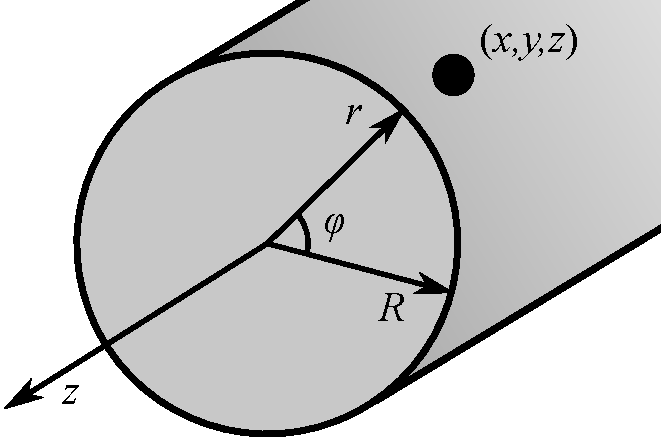
\includegraphics[width = .72\columnwidth]{Analytisk-Mekanik/cylinderopg_sh.pdf}
\caption{Partikel på cylinder.} \label{cyl-fig}
\end{figure}
%
%
\begin{opgave}{Partikel på en cylinder}{1} \label{opg:Cylinder}
Vi ser på en partikel, der kan bevæge sig frit på overfladen af en cylinder med radius $R$, som det ses på figur \ref{cyl-fig}. Her er det oplagt at bruge cylindriske koordinater:
\begin{align*}
x &= r\cos(\phi) \, , \\
y &= r\sin(\phi) \, , \\
z &= z \, .
\end{align*}
\opg Brug de cylindriske koordinater som generaliserede koordinater. Hvilke koordinater ændres, når partiklen bevæger sig?
\opg Udregn $\dt x$, $\dt y$ og $\dt z$ i de nye koordinater.
\opg Opstil den kinetiske energi, $K=\frac{1}{2}mv^2$.
\opg Opstil Lagrangefunktionen. Den potentielle energi er altid nul.
\opg Brug Euler-Lagrangeligningerne til at opstille anden ordens differentialligninger, for de koordinater der ændres, når partiklen bevæger sig.
\opg Hvordan bevæger partiklen sig?
\end{opgave}
%
%
\begin{figure}[h!]
	\centering
	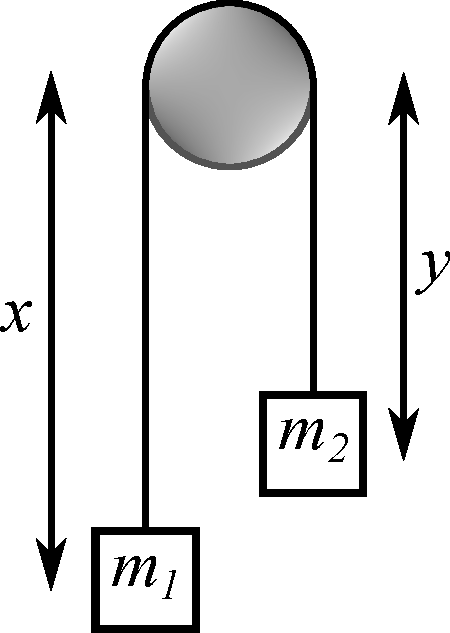
\includegraphics[width=.65\columnwidth]{Analytisk-Mekanik/Atwood.pdf}
	\caption{Illustration af Atwoods faldmaskine, hvor to lod forbindes med en snor over en trisse.} \label{fig:Atwood}
\end{figure}
%
%
\begin{opgave}{Atwoods faldmaskine}{1} \label{opg:Atwood}
I figur \ref{fig:Atwood} ses en illustration af Atwoods faldmaskine, hvori to lodder hænges i hver sin ende af en snor med konstant længde $l$. I figuren er to koordinater også defineret, og de to lodders masser er indtegnet.
\opg Argumenter for at der kun er ét generaliseret koordinat, og udtryk $y$ ved $x$.
\opg Udtryk $\dt{y}$ ved $\dt{x}$.
\opg Definer hhv. $x = 0$ og $y = 0$ som nulpunkt for den potentielle energi for hvert lod, og opskriv den totale potentielle energi\footnote{Har man svært ved at acceptere gyldigheden af at regne med negativ potentiel energi, kan man godt definere nulpunktet under faldmaskinen, hvilket gør at Lagrangefunktionen kommer til at indeholde nogle ekstra konstanter.}.
\opg Opskriv den kinetiske energi som summen af den kinetiske energi for hver af de to lodder.
\opg Vis at Lagrangefunktionen for systemet kan skrives på formen
\begin{align*}
	L(x,\dt{x},t) &= \frac{1}{2}(m_1+m_2)\dt{x}^2 \\
	&+ g\Big(m_1x + m_2(l-x-\pi R)\Big) \: .
\end{align*}
\opg Vis ved brug af Euler-Lagrangeligningen, at systemets bevægelsesligning er
\begin{align*}
	\ddt{x} = g\frac{m_1-m_2}{m_1+m_2} \: .
\end{align*}
\opg Vis ud fra bevægelsesligningen, hvad fortegnet af $\ddt{x}$ er afhængigt af om $m_1>m_2$ eller $m_2>m_1$. Hvilket af de to lodder vil falde ned (hvad betyder det for retningen af bevægelsen)?\\ 
Skrives bevægelsesligningen lidt om fås
\begin{align*}
	\dif[2]{t}{x} &= g\frac{m_1-m_2}{m_1+m_2} = a \\
	\implies \dif{t}{} \left( \dif{t}{x} \right) &= a \\
	\implies \dif{t}{x} &= \ubint{a}{t}\\
	\implies x(t) &= \ubiint{a}{t}{t}
\end{align*}
Det trick vi bruger her er, at integration og differentiation er hinandens omvendte operationer ligesom plus og minus er hinandens omvendte operationer.\footnote{Faktisk har vi også antaget, at to integrationskonstanter er $0$, men det er en mindre detalje.} 
\opg Bestem $x(t)$ ved ovenstående integral.\\ 
Hint: Regn det inderste integrale, så det yderste.
\end{opgave}
%
%
\begin{opgave}{Yoyo}{1} \label{opg:Yoyo}
Betragt yoyoen i figur \ref{fig:yoyo} med massen $m$ og de fysiske dimensioner som vist i figuren.
%
\begin{figure}[]
	\centering
	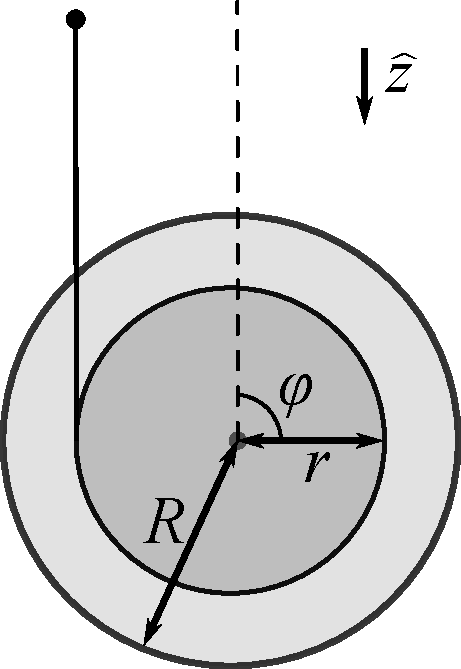
\includegraphics[width=.61\columnwidth]{Analytisk-Mekanik/yoyo.pdf}
	\caption{Skitse af en simpel yoyomodel med radier $r$ og $R$ i et tyngdefelt med i nedadgående retning med styrken $g$.} \label{fig:yoyo}
\end{figure}
%
Tyngdekraften har størrelsen $g$ i $z$-retningen, $\v{F}_\mathrm{g} = mg\zhat$, og den ideelle snor sidder fast i afstanden $r$ fra centrum. At snoren er ideel betyder, at den anses som ustrækkelig, masseløs, og derudover anses friktionen mellem snoren og yoyoen som værende så stor, at yoyoen ikke glider. Det kan vises, at yoyoens inertimoment i denne model er
\begin{align*}
	I = \frac{1}{2}mR^2 \: .
\end{align*}
Som generaliseret koordinat benyttes $z$, fordi $z$ og $\phi$ er koblede.
\opg Antagelsen at friktionen mellem snoren og yoyoen er tilpas stor, gør at det punkt hvor snoren slipper yoyoen står stille, hvilket betyder, at rotationen lige præcis udligner bevægelsen fra, at yoyoen falder nedad.\footnote{Dette kaldes ofte at yoyoen \textit{ruller uden at glide}, hvilket er en meget almindelig antagelse i fysik.} Det betyder, at farten $v$ i ligning \eqref{k-eq:SmartFart} er lig med farten $v_\textsc{cm}$ i ligning \eqref{k-eq:K}, hvor begge ligninger henviser til kompendiet. Brug disse ligninger til at vise at
\begin{align*}
	K = \frac{1}{2}m\dt{z}^2 + \frac{1}{4}mR^2\left(\frac{\dt{z}}{r}\right)^2 \: .
\end{align*}
\opg Argumenter for at den potentielle energi kan skrives på formen $V = -mgz$.
\opg Konkluder at Lagrangefunktionen for problemet er
\begin{align*}
	L = \frac{1}{2}m\left[1 + \frac{1}{2}\left(\frac{R}{r}\right)^2\right]\dt{z}^2 + mgz \: .
\end{align*}
\opg Bestem nu følgende afledede af Lagrangefunktionen
\begin{align*}
	\pdif{z}{L} &= \; ? \\
	\pdif{\dt{z}}{L} &= \; ? \\
	\el{\dt{z}} &= \; ?
\end{align*}
\opg Brug Euler-Lagrangeligningen, ligning \eqref{k-Euler-Lagrange} i kompendiet, til at vise at
\begin{align} \label{eq:YoyoDiffLign}
	\ddt{z} = \frac{g}{1 + \frac{1}{2}\left(\frac{R}{r}\right)^2} \: .
\end{align} \\[1mm]
Det kan vises at løsningen til denne differentialligning er
\begin{align} \label{eq:YoyoBevLign}
	z(t) = \frac{g}{2}\left[1 + \frac{1}{2}\left(\frac{R}{r}\right)^2\right]^{-1}t^2 + v_0t + z_0 \: ,
\end{align}
hvor $v_0$ er startfarten, og $z_0$ er startstedkoordinatet. Ved indsættelse i ligning \eqref{eq:YoyoDiffLign} kan det vises, at ligning \eqref{eq:YoyoBevLign} er en løsning, eller det kan udledes med samme metode som i opgaverne \ref{opg:Atwood} og \ref{opg:cylinder}.
\opg Overvej hvilke fordele og ulemper der er, ved at benytte Lagrangemekanikken til at løse dette problem frem for Newtonsk mekanik.
\end{opgave}
%
%
\begin{opgave}{Klods på en fjeder}{2}
I starten af kompendiets første kapitel blev det vist, at bevægelsesligningen for en klods på en fjeder, figur \ref{k-fig:fjeder} i kompendiet, er
\begin{align*}
	\ddt{x} = -\frac{k}{m}x \: .
\end{align*}
Til dette blev Newtons formulering af mekanikken brugt, men det samme kan også opnås med Lagrangeformalismen.
\opg Opstil Lagrangefunktionen for problemet.
\opg Benyt Euler-Lagrangeligningen til at komme frem til det samme.
\end{opgave}
%
%
\begin{opgave}{Cylinder på skråplan}{2}\label{opg:cylinder}
En cylinder med massen $m$, radius $R$ og inertimoment $I$ placeres på et skråplan med vinklen $\alpha$ i forhold til vandret.\\
\opg Skitser situationen.
\opg Indtegn på skitsen det koordinatsystem, der giver det færrest mulige afhængige koordinater.
\opg Opstil den potentielle energi $V$ for systemet, hvor der ses bort fra cylinderes udtrækning.
\opg Udtryk den kinetiske energi $K$ ved cylinderens fysiske parametre og tidsafledede af de valgte generaliserede koordinater.
\opg Opskriv problemets Lagrangefunktion.
\opg Vis at ved løsning af Euler-Lagrangeligningen fåes
\begin{align*}
\ddt{x} = -\dfrac{g\sin\alpha}{1+I/mR^2} \: .
\end{align*}
\opg Argumenter for at accelerationen er konstant.
\opg Lad nu accelerationen være $\tilde{g}$, og vis at bevægelsesligningens løsning er
\begin{align*}
x(t) = \frac{1}{2}\tilde{g}t^2 + v_0t + x_0 \: .
\end{align*}
\end{opgave}
%
%
\begin{figure}[h!]
	\centering
	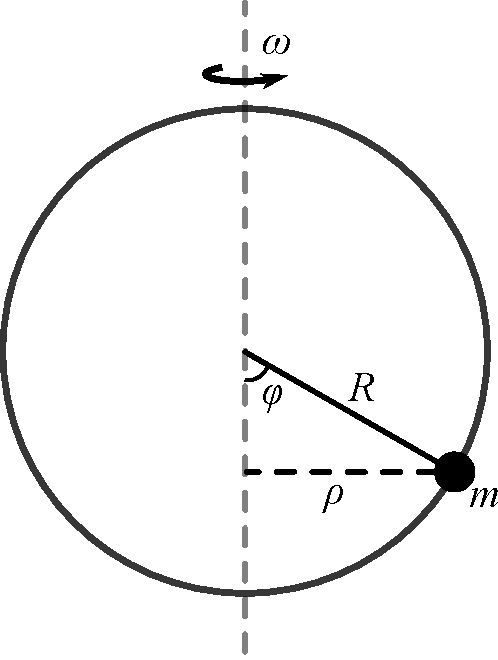
\includegraphics[width=.65\columnwidth]{Analytisk-Mekanik/BeadOnHoop.pdf}
	\caption{Illustration af situationen, hvor koordinater og andre parametre er indtegnet.} \label{fig:BeadOnHoop}
\end{figure}
%
%
\newpage
\begin{opgave}{Masse på roterende ring}{3}
Et lod med masse $m$ er placeret på en ring, hvorpå den kan bevæge sig friktionsløst, som i figur \ref{fig:BeadOnHoop}. Ringen har radius $R$, og den roterer om sin egen akse med vinkelhastigheden $\omega$. Massen kan beskrives udelukkende ved det generaliserede koordinat $\phi$, men for at indse dette gøres brug af koordinatet $\rho$.
\opg Udtryk den potentielle energi ved det generaliserede koordinat $\phi$, således at $V(\phi=0)=0$.
\opg Massens hastighed deles nu op i to komponenter - en der svarer til ind i tegningen og en langs ringen. Disse kaldes henholdsvis $v_\mathrm{ring}$, idet det er bevægelsen som følge af ringens rotation, og $v_\mathrm{lod}$ idet det er lodets bevægelse på ringen. Bestem disse komponenter udtrykt ved $\omega$, $\phi$ og $\dt{\phi}$, samt eventuelle geometriske parametre.\\
Hint: Benyt ligning \eqref{k-eq:SmartFart} i kompendiet.
\opg Brug dette til at bestemme den kinetiske energi, og vis dermed at Lagrangefunktionen er
\begin{align*}
	L = \frac{1}{2}mR^2\big[\dt{\phi}^2 + \omega^2\sin^2(\phi)\big] - mgR\big[1-\cos(\phi)\big] \: .
\end{align*}
\opg Benyt Euler-Lagrangeligningen til at vise, at bevægelsesligningen er
\begin{align*}
	\ddt{\phi} = \left[\omega^2\cos(\phi) - \frac{g}{R}\right]\sin(\phi) \: .
\end{align*}
\opg Hvad er kriteriet for henholdsvis et stabilt og ustabilt ligevægtspunkt fysisk og matematisk?
\opg Brug kriterierne til at bestemme systemets ligevægtspunkter, og forklar hvad de betyder fysisk.
\opg Eksister alle disse punkter for alle $\omega, R$ og $g$?
\opg Diskuter om ligevægtspunkterne er stabile eller ustabile i alle tilfælde fra sidste spørgsmål.\footnote{Ligevægtspunkterne $\phi_0 = 0,\pm\pi$ er ikke super komplicerede at vise stabiliteten af matematisk, men det sidste er svært, hvorfor dette bør tilgås med forsigtighed. Det er dog vist i facitlisten, hvordan dette gøres, hvilket kan være en gennemlæsning værd.}
\end{opgave}
%
%
\section*{Flerlegemeproblemer}
%
%
\begin{figure}[h!]
\centering
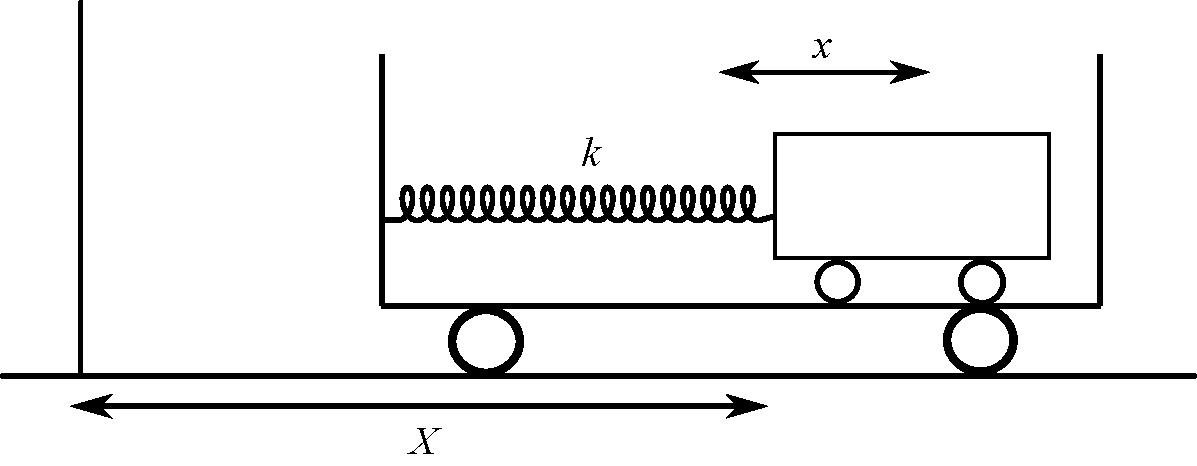
\includegraphics[width=\columnwidth]{Analytisk-Mekanik/ToKobledeVogne.pdf}
\caption{Illustration af problemet i opgave \ref{opg:ToKobledeVogne}. $X$ er stedkoordinatet for den store vogn, og $x$ er stedkoordinatet for den lille, hvor $x=0$ defineres som midtpunktet i den store vogn.}
\label{fig:ToKobledeVogne}
\end{figure}
%
%
\begin{opgave}{To koblede vogne}{2} \label{opg:ToKobledeVogne}
En lille vogn med massen $m$ placeres i en større vogn, og de to forbindes med en fjeder med fjederkonstant $k$. Den lille vogn antages at kunne bevæge sig friktionsløst i forhold til den store og den store i forhold til underlaget, og de generaliserede koordinater defineres som på figur \ref{fig:ToKobledeVogne}. Den store vogn tvinges til simpel harmonisk bevægelse, det vil sige $X = A\cos(\omega t)$, hvor $A,\omega$ er konstanter, og derudover kaldes den lille vogns naturlige vinkelfrekvens $\omega_0 = \sqrt{\frac{k}{m}}$.
\opg Argumenter for at den lille vogns hastighed i forhold til underlaget kan skrives som
\begin{align*}
v = \dt{x} + \dt{X} \: ,
\end{align*}
og brug dette til at indse, at
\begin{align*}
K = \frac{1}{2}m\left(\dt{x} + \dt{X}\right)^2 \: .
\end{align*}
\opg Argumenter for at den potentielle energi for den lille vogn er
\begin{align*}
V = \frac{1}{2}kx^2 \: ,
\end{align*}
og konkluder at
\begin{align*}
L = \frac{1}{2}m\left(\dt{x} + \dt{X}\right)^2 - \frac{1}{2}kx^2 \: .
\end{align*}
\opg Brug dette til at vise, at
\begin{align*}
\pdif{\dt{x}}{L} &= m(\dt{x} + \dt{X}) \: ,\\
\pdif{x}{L} &= -kx \: .
\end{align*}
\opg Vis at
\begin{align*}
\dif{t}{}\left(\pdif{\dt{x}}{L}\right) = m\ddt{x} - Am\omega^2\cos(\omega t) \: ,
\end{align*}
og konkluder at
\begin{align*}
\ddt{x} + \frac{k}{m}x = A\omega^2\cos(\omega t) \: .
\end{align*}
\opg Fastholdes den store vogn nu i $X=0$ bliver systemet i denne opgave ækvivalent til et system, uden den store vogn, hvor fjederen på den lille vogn er spændt fast på væggen, hvilket er en harmonisk oscillator. $X=0$ kan realiseres ved at sætte $A=0$. Vis at bevægelsesligningen i dette tilfælde reducerer til en harmonisk oscillator.
\opg Hvorfor er det relevant at tjekke at systemet reducerer til en harmonisk oscillator i grænsen $A=0$?\\ \\
\end{opgave}
%
%
\begin{figure}[h!]
\centering
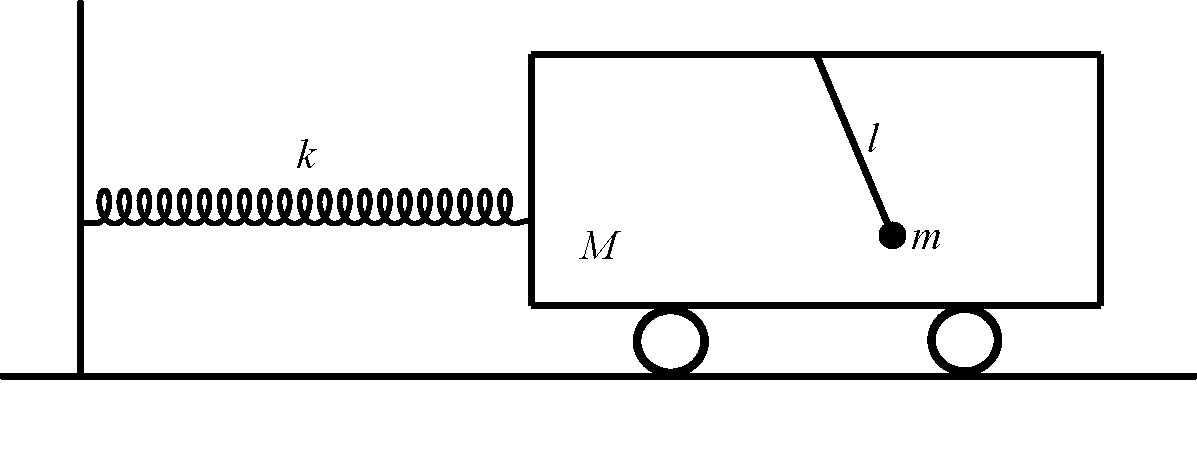
\includegraphics[width=\columnwidth]{Analytisk-Mekanik/PendulIVognOpg.pdf}
\caption{Pendul med massen $m$ og længden $l$ placeret i en vogn med massen $M$, der er fastgjort til en væg med en en fjeder med fjederkonstant $k$.}
\label{fig:PendulIVognOpg}
\end{figure} 
%
%
\begin{opgave}{Pendul i en vogn}{4}
I figur \ref{fig:PendulIVognOpg} er der tegnet et pendul, ophængt i en vogn, der tilmed er fastspændt med en fjeder til en væg, og de relevante fysiske størrelser er indtegnet.
\opg Identificer systemets generaliserede koordinater, indtegn enhedsvektorerne for et kartesisk koordinatsystem og definer origo. %(hint: Se beskrivelsen af pendulet med Lagrangeformalismen og opgave \ref{opg:ToKobledeVogne})
\opg Opskriv pendulets kartesiske koordinater, $(X_p,Y_p)$, udtrykt ved de generaliserede koordinater, samt vognens kartesiske $X$-koordinat, $X_v$, og argumenter for, at $Y_v$ er ubetydelig for problemet.
\opg Bestem systemets potentielle energi.
\opg Bestem systemets kinetiske energi og opskriv Lagrangefunktionen. %(hint: Anvend de kartesiske koordinater fra sidste opgave til først at bestemme de relevante hastigheder)
\opg Vis at løsningen til Euler-Lagrangeligningen er de koblede differentialligninger
\begin{align*}
a&) \quad M\ddt{x} + m\ddt{x} + ml\ddt{\phi}\cos\phi - ml\dt{\phi}^2\sin\phi = -kx \:, \\
b&) \quad ml^2\ddt{\phi} + ml\ddt{x}\cos\phi = -mgl\sin\phi \: .
\end{align*}
\opg Bestem Taylorudviklingen til 1. orden i $\phi$ af bevægelsesligningerne. \\ \\
Nu kigges på grænserne
\begin{align*}
&1. \quad k \rightarrow \infty \: ,\\
&2. \quad M \gg m \: .
\end{align*}
\opg Hvilken fysisk situation svarer hver grænse til?
\opg Hvad forventes systemet at blive til i de ovenstående grænser?
\opg Hvad bliver det til?
\end{opgave}
\newpage
%
%
\section*{Fiktive Kræfter}
%
%
\begin{opgave}{Fysiske og fiktive kræfter}{2} \label{opg:Fiktivekraefter}
Nu betragtes systemet fra karruseleksemplet i afsnit \ref{k-sec:Karrusel}, og der tilføjes en stedafhængig kraft til systemet med potentiel energi $V(x,y)$.
\opg Hvorfor giver antagelserne at følgende er sandt?
\begin{align*}
	\pdif{\dt{x}}{}V(x,y) &= 0 \\
	\pdif{\dt{y}}{}V(x,y) &= 0
\end{align*}
\opg Argumenter for at $V(x,y)$ ikke indgår i $\el{\dt{q}_i}$ for $q_i=x,y$. Med andre ord, at
\begin{align*}
	\el{\dt{x}} &= \dif{t}{}\left(\pdif{\dt{x}}{K}\right) \: , \\
	\el{\dt{y}} &= \dif{t}{}\left(\pdif{\dt{y}}{K}\right) \: .
\end{align*}
\opg Konkluder at bevægelsesligningerne for systemet er
\begin{align*}
	m\ddt{x} &= 2m\omega\dt{y} + m\omega^2x -\pdif{x}{}V(x,y) \: , \\
	m\ddt{y} &= -2m\omega\dt{x} + m\omega^2y -\pdif{y}{}V(x,y) \: ,
\end{align*}
som kan skrives på formen
\begin{align*}
	m\ddt{x} &= F_x^\mathrm{cor} + F_x^\mathrm{cf} - \pdif{x}{}V(x,y,z) \: , \\
	m\ddt{y} &= F_y^\mathrm{cor} + F_y^\mathrm{cf} - \pdif{y}{}V(x,y,z) \: .
\end{align*}
hvor superscriptet angiver, hvilken af de to fiktive kræfter, der er tale om, og subscriptet angiver retningen.
\opg Beskriv hvordan disse fiktive kræfter opfører sig overfor Newtons 2. lov og sammenlign med fysiske kræfter som for eksempel tyngdekraften. \vspace{3mm}\\
Det vigtige i denne opgave er ikke at regne eksemplet igennem på ny, men at gennemgå argumenterne for de konklusioner der drages, for at give en forståelse for begrebet \textit{fiktive kræfter}.
\end{opgave}
%
%
\begin{figure*}
	\centering
	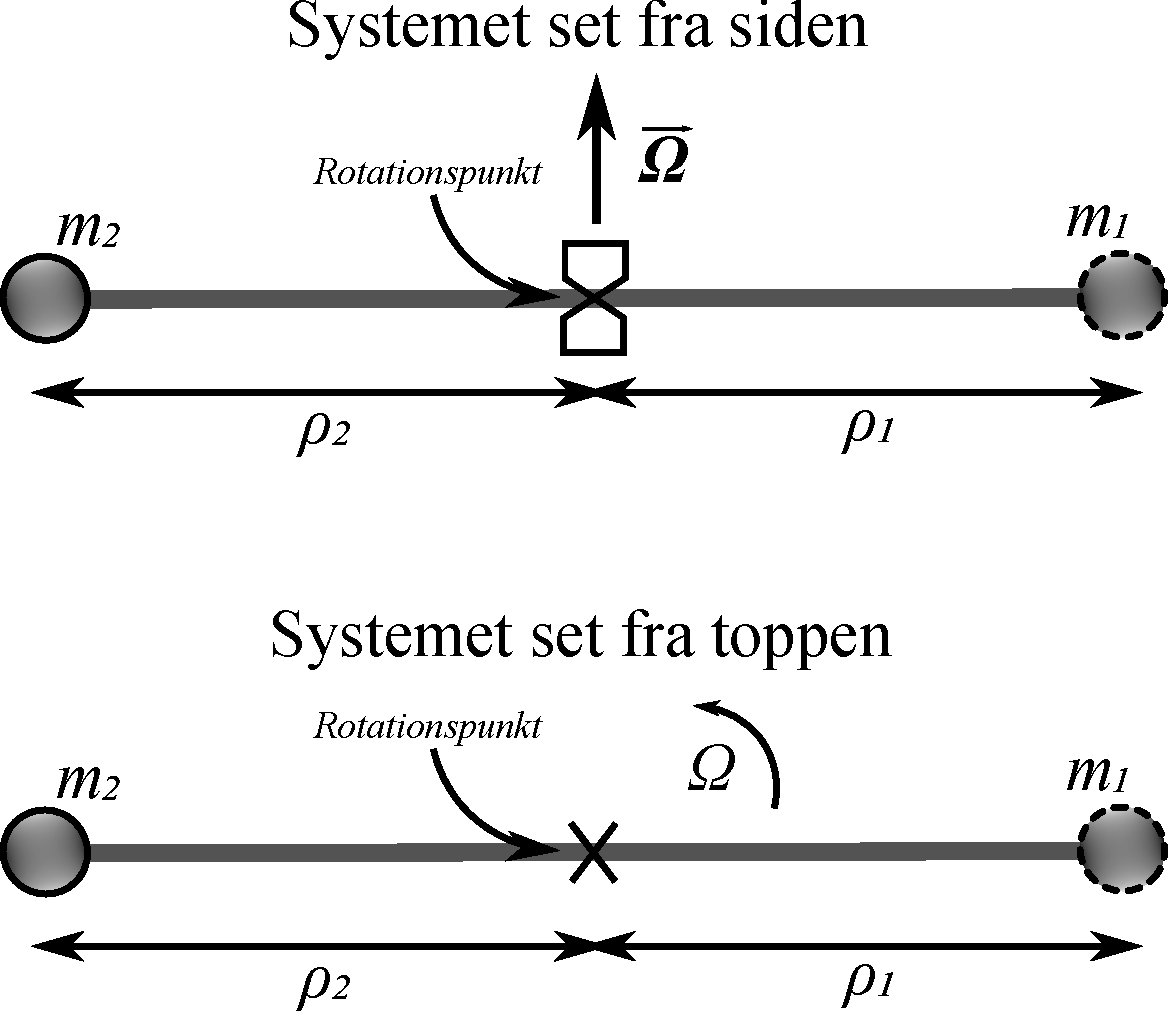
\includegraphics[width=.67\textwidth]{Analytisk-Mekanik/ToMasserRoterendeStang.pdf}
	\caption{Illustration af problemet, hvor stangen kan bevæge sig lineært gennem rotationspunktet udover at rotere med konstant vinkelhastighed $\Omega$.}	\label{fig:ToMasserRoterendeStang}
\end{figure*}
%
%
\begin{opgave}{To masser på en roterende stang}{3}
To legemer med masserne $m_1$ og $m_2$ fastspændes for enden af en stang. Denne stang monteres på et apparat, således at stangen kan rotere omkring apparatet med konstant vinkelhastighed $\v{\Omega}$, samtidig med at den kan bevæge sig friktionsløs frem og tilbage gennem apparatet. Afstanden fra legemerne til apparatet kaldes hhv. $\rho_1$ og $\rho_2$, og da vil $l = \rho_1 + \rho_2$, hvor $l$ er længden af stangen. Opstillingen kan ses på figur~\ref{fig:ToMasserRoterendeStang}.
\opg Identificer et logisk koordinatsystem at beskrive problemet i.
\opg Identificer de(n) generaliserede koordinat(er) for hvert legeme.
\opg Antagelserne giver en begrænsning af hvordan de to legemer kan bevæge sig i forhold til hinanden. Hvad er sammenhængen mellem de to legemers hastighed?
\opg Med henvisning til ligning \eqref{k-eq:FiktiveKraefter} i kompendiet bestem Coriolis og centrifugalkraften på hvert legeme, og inkluder begrænsningen på hastighederne.
\opg Tegn kræfterne der virker på hvert legeme, og beskriv hvilke antagelse tegningen bygger på.
\opg Argumenter for at Corioliskraften er ubetydelig for problemet grundet antagelserne.
\opg Benyt at summen af kræfter på et legeme i ligevægt er nul, $\sum\v{F} = \v{0}$, til at bestemme et systemets ligevægtskonfiguration.
\opg Hvordan forventes ligevægtskonfigurationen at se ud, under antagelse af at $m_1 = m_2$.
\opg Stemmer forventningen og det beregnede udtryk overens?
\end{opgave}
%
%
\begin{opgave}{Er fiktive kræfter trælse?}{3}
Betragt nu de fiktive kræfter, som givet i ligning \eqref{k-eq:FiktiveKraefter} i kompendiet.
\opg Afhænger hver af de fiktive kræfter af sted eller hastighed?
\opg Det er bøvlet, hvis eksempelvis funktionen indgår som sig selv, samt sin første og anden afledede. Med tanke på hvad de kræfter, der er arbejdet mest med i kapitlet, giver nogle af de fiktive kræfter så anledning til differentialligninger, der er specielt vanskelige at løse?
\opg Hvis differentialligningen kan skrives på formen
\begin{align*}
\dif[2]{t}{f(t)} = k\dif{t}{f(t)}
\end{align*}
kan den relativt simpelt løses. Hvorfor?
\end{opgave}
%
%
\section*{Perspektiverende Problemer}
%
%
\begin{opgave}{Tennis Racket Theorem}{4}
Indtil videre har vi kun kigget på rotationer om én akse, men ofte roterer ting om flere akser, hvilket komplicerer tingene en hel del. I denne opgave vil vi ikke forsøge at udlede bevægelsesligningerne for et sådant system, men forsøge at forstå hvilken information de kan give os. Det kan vises at bevægelsesligningerne for et stift legeme, der kan rotere om tre akser med hver sit inertimoment er
\begin{align*}
	I_x\dt{\omega}_x &= (I_y-I_z)\omega_y\omega_z \: , \\
	I_y\dt{\omega}_y &= (I_z-I_x)\omega_z\omega_x \: , \\
	I_z\dt{\omega}_z &= (I_x-I_y)\omega_x\omega_y \: ,
\end{align*}
eller på vektorform
\begin{align} \label{eq:TRT_DiffLign}
	\xyz{I_x\dt{\omega}_x}{I_y\dt{\omega}_y}{I_z\dt{\omega}_z} = \xyz{(I_y-I_z)\omega_y\omega_z}{(I_z-I_x)\omega_z\omega_x}{(I_x-I_y)\omega_x\omega_y} \: .
\end{align}
Her er $I_i$ og $\omega_i$ henholdsvis inertimomentet og vinkelhastigheden for rotation om den $i$'te akse, og yderligere antages det at $I_x>I_y>I_z>0$.
\opg Antag at $\omega_y \approx \omega_z$ er meget små og brug dette til at vise, at
\begin{align} \label{eq:TRT_DiffLignX}
	\dif{t}{}\xyz{I_x\dt{\omega}_x}{I_y\dt{\omega}_y}{I_z\dt{\omega}_z} \simeq \xyz{0}{(I_z-I_x)\dt{\omega_z}\omega_x}{(I_x-I_y)\omega_x\dt{\omega}_y} \: .
\end{align}
Hint: $\omega_y$ og $\omega_z$ er så små, at andenordensled med dem, dvs. led på formen $\omega_i\omega_j$ hvor $i=y,z$ og $j=y,z$, er nul, mens førsteordensled ikke er.
\opg Vis ved brug af ligningerne \eqref{eq:TRT_DiffLign} og \eqref{eq:TRT_DiffLignX}, at
\begin{align} \label{eq:TRT_DDiffLignX}
	\dif{t}{}\xyz{I_x\dt{\omega}_x}{I_y\dt{\omega}_y}{I_z\dt{\omega}_z} \simeq \xyz{0}{\omega_x^2\omega_y(I_z-I_x)(I_x-I_y)/I_z}{\omega_x^2\omega_z(I_x-I_y)(I_z-I_x)/I_y} \: .
\end{align}
\opg Konkluder ud fra ligning \eqref{eq:TRT_DDiffLignX} at fortegnet for $\ddt{\omega}_y$ og $\ddt{\omega}_z$ er modsat af henholdsvis $\omega_y$ og $\omega_z$.
\opg Antag nu at $\omega_x \approx \omega_z$ er meget små, analogt til spørgsmål 1), og brug helt samme metode til at vise, at
\begin{align} \label{eq:TRT_DiffLignY}
	\dif{t}{}\xyz{I_x\dt{\omega}_x}{I_y\dt{\omega}_y}{I_z\dt{\omega}_z} \simeq \xyz{\omega_y^2\omega_x(I_y-I_z)(I_x-I_y)/I_z}{0}{\omega_y^2\omega_z(I_x-I_y)(I_y-I_z)/I_x} \: .
\end{align}
\opg Benyt nu ligning \eqref{eq:TRT_DiffLignY} til at konkludere, at fortegnene for $\ddt{\omega}_x$ og $\omega_x$ er ens og ligeledes for $\omega_z$.
\opg Legemet sættes til at rotere om sin $i$'te akse, hvor vinkelhastigheden om de andre akser er små. Hvis legemet fortsætter med stort set kun at rotere om den $i$'te akse, da betragtes rotation om den $i$'te rotationsakse som stabil. Argumenter for at rotation om den $i$'te rotationsakse er stabil, hvis $\ddt{\omega}_j \propto - \omega_j \, \forall \, j\neq i$.
\opg Ved analoge udregninger fås, at $\ddt{\omega}_x \propto -\omega_x$ og $\ddt{\omega}_y \propto -\omega_y$ hvis $\omega_x\approx\omega_y$ er små. Konkluder at rotation om $x$- og $z$-aksen er stabil, mens rotation om $y$-aksen er ustabil. Dette resultat kaldes \textit{Tennis Racket Theorem}, \textit{Intermediate Axis Theorem} eller \textit{Dzhanibekov Effect}\footnote{Løses differentialligningen i ligning \ref{eq:TRT_DiffLign} fås en bevægelse som denne: \url{https://www.youtube.com/watch?v=1n-HMSCDYtM}} efter Dzhanibekov, der bemærkede det under en mission i rummet.
\opg Den eneste antagelse der er lavet, er at legemet er stift\footnote{Det er også antaget at legemet ikke er påvirket af ydre kræfter i udledningen af ligning \ref{eq:TRT_DiffLign}, men det betyder bare at konklusionen om stabilitet af rotationsakser ikke afhænger af nogle ydre kræfter.}. Brug dette til at undersøge dette fænomen med virkelige objekter, forklar hvilke rotationsakser, der er mulige for objektet, samt den relative størrelse af inertimomentet for rotation omkring de forskellige akser.
\end{opgave}
%
%
\begin{opgave}{Hamiltonfunktionen og et systems energi}{3} \label{opg:HamiltonEnergi}
Antag at et systems kinetiske energi kan skrives på formen $K = \frac{1}{2}A(q)\dt{q}^2$, hvor $A(q)$ er en arbitrær funktion af $q$, som er det eneste generaliserede koordinat. Den potentielle energi kaldes $V(q)$, og der antages kun, at den er stedsafhængig.
\opg Opskriv systemets Lagrangefunktion.
\opg Bestem den generaliserede impuls ud fra dennes definition.
\opg Udtryk $\dt{q}$ ved $p$ og $A(q)$.
\opg Benyt definitionen af Hamiltonfunktion til at bestemme denne.
\opg Vis at hvis et systems kinetiske energi kan skrives på formen $K = \frac{1}{2}A(q)\dt{q}^2$, så er $H = E$.
\opg Argumenter for at disse argumenter generaliserer til $n$ generaliserede koordinater, hvor den kinetisk energi på tilsvarende vis antages at være
\begin{align*}
	K = \sum_i\frac{1}{2}A(q_i)\dt{q}_i^2 \: .
\end{align*}
\end{opgave}
%
%
\begin{opgave}{Fra klassisk mekanik til kvantemekanik}{3}
Her vil sammenhængen mellem klassisk mekanik og kvantemekanik belyses gennem en metode til at opskrive Hamiltonoperatoren for et system, ved at starte med en klassisk analyse af problemet. Der kigges her på én partikel.
\opg Antag at den generaliserede impuls kan skrives på formen $p = m\dt{q}$. Benyt dette til at opskrive den kinetiske energi udtrykt ved impulsen $p$.
\opg Benyt resultatet fra opgave \ref{opg:HamiltonEnergi} til at opskrive systemets Hamiltonfunktion.
\opg For at kunne beskrive systemet kvantemekanisk, skal Hamiltonfunktionen skrives om til en Hamiltonoperator. Hvilke elementer i Hamiltonfunktionen skal omskrives, for at stå på operatorform?
\opg Omskriv de før angivne elementer til operatorform ved hjælp af tabel \ref{k-tab:operatorer_i_kvant} i kompendiet, og bestem derved Hamiltonoperatoren.
\end{opgave}
%
%
\begin{opgave}{Energibevarelse i Hamilton}{4}
I opgave \ref{opg:HamiltonEnergi} blev det vist at Hamiltonfunktionen i nogle tilfælde er lig med et systems energi. Det kunne derfor være interessant at undersøge, under hvilke omstændigheder Hamiltonfunktionen er bevaret over tid.
\opg Beskriv forskellen på den fuldstændige differentiation, f.eks. $\d/\d t$, og den partielle differentiation, eksempelvis $\partial/\partial t$. \footnote{Differentialoperatorerne er her skrevet med hensyn til tid, men det er bare for at give et eksempel. Der tænkes her på den generelle forskel.} 
\opg Opskriv den fuldstændigt tidsafledede af en generel Hamiltonfunktion af ét generaliseret koordinat, $\d H/\d t$, vha. kædereglen.
\opg Benyt nu Hamiltons ligninger til at simplificere summen.
\opg Konkluder at
\begin{align*}
\dif{t}{H} = \pdif{t}{H} \: .
\end{align*}
\opg Under hvilke omstændigheder er Hamiltonfunktionen bevaret i tid?
\opg Med henvisning til opgave \ref{opg:HamiltonEnergi}, hvad betyder det fysisk for systemet, at Hamiltonfunktionen er bevaret i tid?
\opg Opskriv $\d H/\d t$ for en generel Hamiltonfunktion af $n$ generaliserede koordinater, og vis at ovenstående er sandt for $n$ generaliserede koordinater.
\end{opgave}
\chapter{Kvantemekanik}
\section*{Uendeligt dyb brønd}
\begin{opgave}{Parabelformet bølgefunktion}{1}\label{kvant:opg:parabel}
Vi ser her på en partikel i en uendelig brønd i intervallet fra $0$ til $L$. Lad bølgefunktionen være:
$$
\psi = Nx(L-x) 
$$
\opg Find $N$ så bølgefunktionen er normeret.
\opg Hvad er forventningsværdien for positionen $\expect x$?
\opg Find forventningsværdien for energien $\expect E$ og sammenlign den fundne energi med grundtilstandsenergien: $\frac{\pi^2\hbar^2}{2mL^2}$.
\opg Er $\psi$ en stationær tilstand?
\end{opgave}
%
\begin{opgave}{Sammensatte bølgefunktioner}{1}
Find normeringskonstanten $N$ og energien $E$ for de følgende bølgefunktioner, der er sammensat af stationære tilstande for den uendelige brønd.
\opg $N(\psi_1+\psi_2)$.
\opg $N(\psi_1-\psi_3)$.
\opg $N(\psi_1+\psi_2-2\psi_3)$.\\
Hint: Udnyt at bølgefunktionerne er ortonormale.
\end{opgave}
%
\begin{opgave}{Den tidsafhængige bølgefunktion}{2}
I en uendelig brønd er bølgefunktionen til tiden $t=0$:
$$
\Psi(x,0) = \frac{1}{\sqrt{5}}(2\psi_1+\psi_2) 
$$
\opg Hvad er $\Psi(x,t)$? Du kan med fordel bruge 
$$
\omega = \frac{E_1}{\hbar} = \frac{\pi^2\hbar}{2mL^2} \, .
$$
\opg Hvad er $\Psi^*(x,t)$?
\opg Skriv $\Psi^*x\Psi$ så simpelt som muligt.
\opg Hvad er $\expect{x(t)}$? \\
Hint:
\begin{align*}
e^{i\theta}+e^{-i\theta} &= 2\cos \theta \, , \\ \matrixel{\psi_n}{x}{\psi_n} &= \frac{L}{2} \, , \\  \matrixel{\psi_1}{x}{\psi_2} &= \frac{-16L}{9\pi^2} \, .
\end{align*}
\end{opgave}
%
\begin{opgave}{En partikel i et kvadrat}{3}
I to dimensioner er den tidsuafhængige Schrödingerligning i kartesiske koordinater:
$$
E\psi(x,y) = \frac{-\hbar^2}{2m}\left(\pdif[2]{x}\psi +\pdif[2]{y}\psi\right) + V(x,y)
$$
Vi vil se på en kvadratisk brønd, i to dimensioner, med sidelængder på $L$. Her er potentialet nul, når $0\leq x\leq L$ og $0\leq y\leq L$.
Antag nu at man kan skrive bølgefunktionen som:
 $$\psi(x,y) = X(x)Y(y) = XY$$
\opg Indsæt $\psi = XY$ i Schrödingerligningen med $V=0$ og isoler $E$.
\opg Energien vil bestå af en bidrag fra $X$ og $Y$, så $E=E_x+E_y$. Opstil differentialligninger i stil med ligning \eqref{k-kvant:eq:infb} i kompendiet for $X$ og $Y$.
\opg Find generelle løsninger til differentialligningerne, bølgefunktionen og de tilhørende energier. Bemærk at der vil være et kvantetal for hver af differentialligningerne. 
\opg Hvad er de fem laveste energier? Skitser bølgefunktionerne med disse energier.
\end{opgave}
%
\begin{opgave}{En partikel i en boks}{3}
I tre dimensioner er den tidsuafhængige Schrödingerligning i kartesiske koordinater:
$$
E\psi(x,y,z) = \frac{-\hbar^2}{2m}\left(\pdif[2]{x}\psi +\pdif[2]{y}\psi+\pdif[2]{z}\psi\right) + V(x,y,z)
$$
Vi vil se på en kubisk boks med en sidelængde på $L$, hvor potentialet er nul, når $x$, $y$ og $z$ alle er imellem 0 og $L$.
Antag at man kan skrive bølgefunktionen som:
$$
\psi(x,y,z) = X(x)Y(y)Z(z) = XYZ
$$
\opg Indsæt $\psi = XYZ$ i Schrödingerligningen med $V=0$ og isoler $E$.
\opg Energien vil bestå af et bidrag fra $X$, $Y$ og $Z$, så $E=E_x+E_y+E_z$. Opstil differentialligninger i stil med ligning \eqref{k-kvant:eq:infb} i kompendiet for $X$, $Y$ og $Z$.
\opg Find generelle løsninger til differentialligningerne, bølgefunktionen og de tilhørende energier. Bemærk at der vil være et kvantetal for hver af differentialligningerne. 
\opg Find de laveste 5 mulige energier udtrykt i $E_1 = \frac{\pi^2\hbar^2}{2mL^2}$ energien for en  endimensionel uendelig brønd med samme brede som boksens sidelængde.
\end{opgave}
\begin{opgave}{Parabelformet bølgefunktion igen}{1}
Denne opgave bygger videre på opgave \ref{kvant:opg:parabel}, så det er en fordel at have lavet denne opgave først. Vi ser igen på en parabelformet bølgefunktion i en uendelig brønd:
$$
\psi=Nx(L-x)
$$
\opg Hvad er $\sigma_x^2 = \expect{x^2}-\expect{x}^2$?

Vi kender allerede $\expect{x}$ og $\abs N^2$ fra opgave \ref{kvant:opg:parabel}.
\begin{align*}
\expect{x} &= \frac{L}{2}\\
\abs N^2 &= \frac{30}{L^5}
\end{align*}
For at finde $\expect{x^2}$ bruges sandwichen:
\begin{align*}
    \expect{x^2}&= \abs N^2 \integral{x^3(L-x)}{x}{0}{L}\\
    &= \frac{30}{L^5}\integral{x^5-2x^4L+x^3L^2}{x}{0}{L}\\
    &= \frac{30}{L^5}\left[\frac{x^6}{6}-\frac{2x^5L}{5}+\frac{x^6}{6}\right]_0^L\\
    &= 30 L^2\left(\frac{15}{60}-\frac{24}{60}+\frac{10}{60}\right)\\
    &= \frac{L^2}{2}
\end{align*}
Nu er usikkerheden:
$$
\sigma_x^2 = \expect{x^2}-\expect{x}^2 = \frac{L^2}{2}-\frac{L^2}{4}=\frac{L^2}{2}
$$
og
$$
\sigma_x = \frac{L}{\sqrt{2}}
$$
\opg Hvad er $\sigma_p^2 = \expect{p^2}-\expect{p}^2$?
Her skal vi bruge at $\op p = -i\hbar\pdif{x}{}$. Så bliver sandwichen:
\begin{align*}
    \expect{p} &= -i\hbar\abs N^2\integral{x(L-x)\pdif{x}{}\left(x(L-x)\right)}{x}{0}{L}\\
    &= \frac{-30i\hbar }{L^5}\integral{x(L-x)(L-2x)}{x}{0}{L}\\
    &= \frac{-30i\hbar }{L^5}\integral{xL^2-3x^2L+2x^3}{x}{0}{L}\\
    &= \frac{-30i\hbar }{L^5}\left[\frac{x^2L^2}{2}-x^3L+\frac{x^4}{2}\right]_0^L\\
    &= \frac{-30i\hbar }{L} \left(\frac{1}{2}-1+\frac{1}{2}\right)\\
    &=0
\end{align*}
Tilsvarende for $\expect{p^2}$, hvor $op p^2 = -\hbar^2\pdif[2]{x}{}$.
\begin{align*}
    \expect{p^2} &= \abs N^2 \integral{x(L-x)\pdif[2]{x}{}\left(x(L-x)\right)}{x}{0}{L}\\
    &= \frac{-30\hbar^2 }{L^5}\integral{x(L-x)(-2)}{x}{0}{L}\\
    &= \frac{60\hbar^2}{L^5}\integral{xL-x^2}{x}{0}{L}\\
    &= \frac{60\hbar^2}{L^5}\left[\frac{x^2L}{2}-\frac{x^3}{3}\right]_0^L\\
    &= \frac{60\hbar^2}{L^5}\left(\frac{L^3}{2}-\frac{L^3}{3}\right)\\
    &= \frac{60\hbar^2}{L^2}\left(\frac{3}{6}-\frac{2}{6}\right)\\
    &= \frac{10\hbar^2}{L^2}
\end{align*}
Så usikkerheden er:
$$
\sigma_p^2 = \expect{p^2} = \frac{10\hbar^2}{L^2}
$$
og:
$$
\sigma_p = \frac{\hbar\sqrt{10}}{L}
$$
\opg Passer det med Heisenbergs usikkerhedsprincip?

Sættes $\sigma_x$ og $\sigma_p$ ind i Heisenbers usikkerhedsprincip findes:
$$
\sigma_x\sigma_p = \frac{L}{\sqrt{2}}\frac{\hbar\sqrt{10}}{L}= \hbar\sqrt{5}\geq\frac{\hbar}{2}
$$
Heisenberg er tilfreds $\ddot \smile$
\end{opgave}

\begin{opgave}{Den frie partikel}{2}
En fri partikel er en partikel der ikke påvirkes af noget potentiale, så $V(x)=0$ for alle $x$
\opg Hvad er $\op H$?

Der er ikke noget potentiale så:
$$
\op H = \frac{-\hbar^2}{2m}\pdif[2]{x}{} = \frac{\op p^2}{2m}
$$
\opg Hvad er $[\op p,\op H]$?

Bemærk at operatorer altid kommuterer med sig selv, så:
\begin{align*}
    [\op p,\op H]&= \op p\op H-\op H\op p\\
    &= \frac{\op p^3}{2m}-\frac{\op p^3}{2m}\\
    &= 0
\end{align*}
\opg Hvilke bølgefunktioner opfylder: $\op p \psi_p = -i\hbar\pdif{x}{\psi_p} = p\psi_p$?

Omskrives dette findes differentialligningen:
$$
\pdif{x}{\psi_p}=\frac{ip}{\hbar}
$$
Løsningen til denne differentialligning er blot en eksponentialfunktion. Imaginærfaktoren ændrer ikke dette, så:
$$
\psi_p = e^{\frac{ipx}{\hbar}}
$$
\opg Hvad sker der hvis man sætter $\psi_p$ ind i Schrödingerligninen?
\begin{align*}
    \op H\psi_p &= \frac{-\hbar^2}{2m}\pdif[2]{x}{\psi_p}\\
    &= \frac{-\hbar^2}{2m}\left(\frac{ip}{\hbar}\right)^2\psi_p\\
    &= \frac{-\hbar^2}{2m}\frac{-p^2}{\hbar^2}\psi_p\\
    &=\frac{p^2}{2m}\psi_p
\end{align*}
\opg Hvad er sammenhængen imellem $E$og $p$?

Energien er:
$$
E=\frac{p^2}{2m}
$$
\opg Hvad er $\sigma_p$ og $\sigma_E$?

Først findes $\expect{p}$, $\expect{p^2}$, $\expect{E}$ og $\expect{E^2}$.
\begin{align*}
    \expect{p} &= \braket{\psi_p}{\op p\psi_p}\\
    &= p\braket{\psi_p}{\psi_p}\\
    &=p
\end{align*}
Dette er en konsekvens af at det er en egentilstand. Udregningen er tilsvarende for de andre.
\begin{align*}
    \expect{p^2} &= p^2\\
    \expect{E} &= E\\
    \expect{E^2} &= E^2
\end{align*}
Det gør det muligt at finde usikkerhederne:
\begin{align*}
    \sigma_p &= \expect{p^2}-\expect p^2 = 0\\
    \sigma_E &= \expect{E^2}-\expect E^2 = 0
\end{align*}
Man kan godt kende $p$og $E$ på samme tid for den frie partikel, og det er ved $\psi_p$ tilstandene.
\end{opgave}
\section*{Harmoniske oscillatorer}
\begin{opgave}{Harmonisk oscillator med $\boldsymbol{\op a_- \op a_+}$}{1}
\label{kvant:opg:amap}
Færdiggør udledningen af den harmoniske oscillator. Hvis du havde problemer med denne udledning er denne opgave stærkt anbefalet.
\opg Udregn $\op a_-\op a_+$.
\opg Brug dette til at udlede ligning \eqref{k-kvant:eq:Hamap} i kompendiet.
\opg Vis at hvis $\psi_n$ er en løsning til Schrödingerligningen, så er $\op a_-\psi_n$ det også.
\opg Hvad er energien af $\op a_- \psi_n$
\end{opgave}
%
\begin{opgave}{Sjov med operatorer}{2}
\label{kvant:opg:sjov}
Vi vil her komme ind på en af grundene til, at hæve-/sænkeoperatorerne er smarte. Udnyt at bølgefunktionerne er ortonormale, og husk at
$$
\op a_\pm = \frac{1}{\sqrt{2 m \hbar\omega}}(\mp i\op p+m\omega \op x) \, .
$$
\opg Udtryk $\op x$ og $\op p$ ved $\op a_+$ og $\op a_-$.
\opg Find $\expect x$ og $\expect p$ for $\psi_0$, $\psi_1$ og $\psi_{n}$.
\opg Gør det samme for $\expect{x^2}$ og $\expect{p^2}$.
\opg Hvad er $\sigma_x$ og $\sigma_p$ for $\psi_n$?
\opg Hvordan passer det med Heisenbergs usikkerhedsprincip?
\end{opgave}
%
\begin{opgave}{Nu med tid}{2}
Til tiden $t=0$ har vi bølgefunktionen: $$\Psi(x,t=0) = N(\psi_0+\psi_1)$$ (Det kan være en fordel at have lavet opgave \ref{kvant:opg:sjov} først.)
\opg Hvad er $N$?
\opg Hvad er $\Psi(x,t)$?
\opg Hvad er $\expect E$?
\opg Hvad er $\expect {x(t)}$?
\end{opgave}
%
\begin{opgave}{Molekylære vibrationer}{2}
En god model for bindingen i et molekyle er Morsepotentialet:
$$
V(r) = D\left(1-e^{-(r-R)}\right)^2
$$
\opg Hvor er potentialets minimum (ligevægtsafstanden)?
\opg Hvad er minimumsværdien af potentialet?
\opg Hvad er potentialet for meget store $r$.
\opg Hvad er $\pdif[2]{r}{V}$ i ligevægtspunktet. Dette er kraftkonstanten $k$ analogt med for en fjeder.
\opg Molekylet vil kunne vibrere omkring ligevægtspunktet. Hvad er $\omega$?
\opg Morse potentialet kan tilnærmes som en harmonisk oscillator. Hvad er grundtilstandsenergien for denne?\\ \\
For et brintmolekyle er Morsepotentialet givet ved:
\begin{align*}
D&=\SI{7.24e-19}{J} \, ,\\
a &= \SI{3.93e10}{m^{-1}} \, ,\\
R &= \SI{7.40e-11}{m} \, ,\\
m_p&=\SI{1.67e-27}{kg} \, .
\end{align*}
\opg Hvad er $\omega$ og $E_0$ for brintmolekylet.
\end{opgave}
\section*{Energibevarelse}
\begin{opgave}{Energibevarelse i kvantetilstande}{3}
Vi skal i denne opgave se på hvordan energibevarelse kommer til udtryk i kvantemekaniske tilstande. Til enhver Hamilton $\hat{H}$ operator kan vi finde et sæt af løsninger som opfylder følgende ligning: $\hat{H}\psi_n=E_n\psi_n$.
\opg Udtryk en generel funktion $f(x)$ som en kombination af løsninger til Schrödinger ligningen.

Alle funktion kan skrives som en som af egentilstande, da disse løsninger danner en komplet basis:
$$
f(x) = \sum_nc_n\psi_n
$$
Man kunne finde koefficienterne $c_n$ med ligning (2.30) men deres præcise form er underordnet 
\opg Hvordan vil denne funktion udvikle sig over tid? (Hint: udtryk $f(x,t)$ som en kombination af løsninger til Schrödinger ligningen)

Tidsudviklingen af $f(x)$ kan findes ved at multiplicere hvert led i summen med den tilsvarende faktor $\exp\left(\frac{-iE_nt}{\hbar}\right)$. Det giver:
$$
f(x,t) = \sum_n c_n\psi_ne^{-iE_nt/\hbar}
$$
\opg Udregn forventningsværdien af energien $\expect E$. Hvordan vil denne udvikle sig over tid?

Forventingsværdien er givet:
\begin{align*}
\expect E &= \matrixel{f(x,t)}{\op H}{f(x,t)}
\end{align*}
Hamiltonoperatoren kan flyttes ind i summen til højre, og anvendes på de individuelle tilstande.
\begin{align*}
&= \matrixel{\sum_n c_n\psi_ne^{-iE_nt/\hbar}}{\op H}{\sum_m c_m\psi_me^{-iE_mt/\hbar}}\\
&= \braket{\sum_n c_n\psi_ne^{-iE_nt/\hbar}}{\sum_m c_m\op H\psi_me^{-iE_mt/\hbar}}\\
&= \braket{\sum_n c_n\psi_ne^{-iE_nt/\hbar}}{\sum_m c_mE_m\psi_me^{-iE_mt/\hbar}}
\end{align*}
Istedet for at have sumtegnene inde i braketten, kan de flyttes udenfor, så det bliver en dobbelt sum.
\begin{align*}
&=\sum_n\sum_m\braket{c_n\psi_ne^{-iE_nt/\hbar}}{c_mE_m\psi_me^{-iE_mt/\hbar}}\\
&=\sum_n\sum_mc_n^*c_mE_m\braket{\psi_ne^{-iE_nt/\hbar}}{\psi_me^{-iE_mt/\hbar}}\\
&=\sum_n\sum_mc_n^*c_mE_me^{i(E_n-E_m)t/\hbar}\braket{\psi_n}{\psi_m}
\end{align*}
Når man tager en dobbelt sum vil man lægge alle kombinationer af $n$ og $m$ sammen. Siden løsningerne til schrödingerligningen er ortonormale vil braketten enten være et når $n=m$ og nul ellers. Det betyder at kun ledene hvor $n$ og $m$ er ens skal tælles med og vi kan reducere den dobbelte sum til en enkelt sum.
\begin{align*}
&= \sum_nc_n^*c_nE_nE^{i(E_n-E_n)t/\hbar}\braket{\psi_n}{\psi_n}\\
&= \sum_n \abs{c_n}^2E_n
\end{align*}
Her fosvandt tidsafhængigheden, så energiens forventningsværdi er konstant.
\end{opgave}
\newpage
\section*{Symmetri}
\begin{opgave}{Lige og ulige funktioner}{1}
En funktion så som $f(x) = x^2$ der opfylder kravet, $f(x) = f(-x)$, kaldes en lige funktion. En funktion som $f(x) = x$ der opfylder det lignende krav, $f(x)=-f(-x)$, kaldes for en ulige funktion.
Det vil sige, at en lige funktion er uændret, hvis man spejler den i $y$-aksen, mens en ulige funktion skifter fortegn ved den samme spejling.
Bemærk at de fleste funktioner er hverken lige eller ulige, og unikt er funktionen $f(x) = 0$ både lige og ulige.
Afgør om følgende funktioner er lige eller ulige.
\opg $\sin x$.
\opg $e^{x^2}$.
\opg $\cos x$.
\end{opgave}
%
\begin{opgave}{Mere om lige og ulige funktioner}{1}
Lad $f_g(x)$ være en lige funktion og $f_u(x)$ være en ulige funktion.\footnote{$g$ og $u$ står for gerate og ungerate, de tyske ord for lige og ulige.}
\opg Vis at produktet af lige og ulige funktioner fungerer på samme måde som produktet af lige og ulige tal, i forhold til hvorvidt produktet er lige eller ulige.
\opg Er $1/f_{g}(x)$ lige eller ulige?
\opg Hvad med $1/f_{u}(x)$?
\opg Hvad er reglen for division af lige og ulige funktioner?
\end{opgave}
\begin{opgave}{Sammensætning af lige og ulige funktioner}{2}
Alle funktioner kan skrives som en unik sum af en lige og en ulige funktion:
$$
f(x) = f_g(x)+f_u(x)
$$
\opg Skriv $f(-x)$ ud fra $f_g(x)$ og $f_u(x)$.
\opg Skriv $f_g(x)$ og $f_u(x)$ ud fra $f(x)$ og $f(-x)$.
\opg Hvad er den lige og den ulige del af eksponentialfunktionen $e^x$?
\end{opgave}
%
\begin{opgave}{Integraler af lige og ulige funktioner.}{3}
Vi vil her finde nogle meget praktiske regneregler for integraler af lige og ulige funktioner over et symmetrisk interval.
Lad $f_g(x)$ være en lige funktion og $f_u(x)$ være en ulige funktion.
Antag derudover at integralerne
$$
\integral{f_g(x)}{x}{0}{a}   \quad \text{og} \quad \integral{f_u(x)}{x}{0}{a} 
$$
er kendte.
\opg Vis at
$$
\integral{f_g(x)}{x}{-a}{a} = 2\integral{f_g(x)}{x}{0}{a} \, .
$$
\opg Vis at
$$\integral{f_u(x)}{x}{-a}{a} = 0 \, .
$$
\opg Brug dette til at løse integralet: $$\integral{x\cos(x)\sin(x)+x^2-x\exp(x^2)}{x}{-1}{1}$$
\end{opgave}
\section{Opgaver}
\begin{opgave}{God opgave}{1}

Find noget
\opg Udled ligning \ref{Pstar}.
\opg Og nu denne ting. Wow.
\end{opgave}


\begin{opgave}{Gravitationelle linser}{1}
Ligning, hvor man beregner hvornår der fokuseres mest
\opg Denne ting
\opg Og nu denne ting. Wow.

(Hint: Udnyt at noget andet gælder)
\end{opgave}

\begin{opgave}{Atmosfærekrav}{3}
For at en planet kan have en stabil atmosfære er den nød til at kunne holde simple molekyler fanget i dens tyngdefelt. Massen af $O_2$ er $m_{O_2} = \SI{5,31e-26}{\kilo\gram}$.
\opg Benyt Newtons gravitationslov og Newtons 2. lov til at bestemme tyngdeaccelerationen på en planets overflade.
\opg Er det legemes kinetiske energi præcis ligeså stor som dens gravitationelle potentielle energi, vil den kunne undslippe det tyngdefelt det befinder sig i. Vis at denne hastighed, kaldet undvigelseshastigheden fra en planet, er givet som
\begin{align*}
	v_\mathrm{ecs}^2 = \frac{2M_pG}{R_p}
\end{align*}
\opg Det oplyses nu fra kinetisk gasteori at
\begin{align*}
	\frac{1}{2}m\bar{v}^2 = \frac{3}{2}k_BT
\end{align*}
hvor $\bar{v}$ er partiklerne i gassens gennemsnitlige fart, $m$ er partiklernes masse, $k_B$ er Boltzmanns konstant og $T$ er temperaturen i Kelvin. \\
Vis at
\begin{align*}
	\frac{M_p}{R_p} = \frac{3}{2}\frac{k_BT}{mG}
\end{align*}
hvis $v_\mathrm{ecs} = \bar{v}$.
\opg Er $v_\mathrm{ecs} = \bar{v}$ vil op mod halvdelen af molekyler med massen $m$ forsvinde væk fra planeten. Konkluder at for at en exoplanet kan fastholde $O_2$ i sin atmosfære, skal der om planeten gælde at
\begin{align} \label{eq:atm}
	\frac{M_p}{R_p} > \frac{3}{2}\frac{k_BT}{m_{O_2}G}
\end{align}
\opg Den gennemsnitlige temperatur på Jorden antages at være \SI{16}{\degree}. Opfylder Jorden ligning \ref{eq:atm}?
\end{opgave}

\begin{opgave}{Gravitationslinser}{1}
I afsnit \ref{sec:GravLinse} om gravitationslinsemetode blev det nævnt at begivenheden skal observeres af flere forskellige målinger.
\opg Hvorfor er 1 måling ikke nok?
\opg Hvorfor er det usandsynligt at observere samme planet med gravitationslinsemetoden mere en én gang?
\opg Hvordan medfører ovenstående at planeten skal kunne ses i flere forskellige uafhængige målinger, for at kunne kaldes en planet?
\end{opgave}

\begin{opgave}{Bose-Einstein kondensat og laserkøling}{3}
For at lave Bose-Einstein kondensater i laboratoriet skal man have nogle lette partikler, der køles ekstremt meget ned.\footnote{For den interesserede læser er et Bose-Einstein kondensat at atomernes bølgefunktioner udvider sig, som temperaturen falder, indtil de sidst overlapper så meget at du får samme bølgefunktion. De kan derfor betragtes som én stor partikel.} Mere præcist køles atomer (ofte alkalimetaller) ned til ~\SI{.1}{\micro\kelvin}, hvilket gøres ved først laserkøling og senere fordampningskøling. Laserkøling fungerer ved at udnytte at fotoner har impuls. Rammes et atom af en foton, der bevæger sig i modsat retning af atomet, exciteres den til et højere energiniveau, men dens fart falder også en smule, for at bevare impulsen. Når atomet henfalder udsendes fotonen igen, og den accelereres en smule i en tilfældig retning. Sker dette mange gange går disse små accelerationer ud med hinanden over tid, hvorved atomet bremses og atomskyen køles. Det virker dog kun, hvis an kan sikre sig at atomer kun interagerer med fotoner, der bevæger sig i modsat retning af dem selv.
\opg Hvad er sammenhængen mellem en fotons energi og bølgelængde?
\opg Hvad sker der hvis et atom rammes af en foton med en energi, der ikke svarer til en (tilladt) atomar overgang? \textit{Hint: Tænk på atomet kvantemekanisk.} \\

Ved laserkølings sendes laserstråler ind fra seks retninger (positiv og negativ retning af hver af de kartesiske akser). Nu simplificeres systemet ved kun at kigge på systemet i én dimension. Betragt nu to ens atomer, der bevæger sig i hver sin retning. Fotonerne kommer fra en laser, der står stille i laboratoriet.
\opg Skiftes referencesystem til hvert atoms referenceramme, ser laseren ud til at bevæge sig. Hvorfor bevæger laseren sig ikke lige hurtigt i begge atomers referencesystem?
\opg Eftersom laseren bevæger sig Dopplerforskydes lyset. Hvad betyder forskellen i bevægelse for Doppllerforskydningen?
\opg Kan begge atomer exciteres af fotoner med samme bølgelængde?
\opg Hvordan kan dette bruges til at bremse atomerne selektiv?
\opg Er opgavetitlen clickbait?
\end{opgave}

\newpage\newpage
\setcounter{opgave}{0}

\section{Facit}
\begin{opgave}{Atmosfærekrav}{3}
For at en planet kan have en stabil atmosfære er den nød til at kunne holde simple molekyler fanget i dens tyngdefelt. Massen af $O_2$ er $m_{O_2} = \SI{5,31e-26}{\kilo\gram}$.
\opg Newtons gravitationslov siger at tyngdekraften mellem legemer i afstand $r$ er
\begin{align*}
	F_G = G\frac{mM}{r^2}
\end{align*}
Bruges Newtons anden lov er
\begin{align*}
	mg &= G\frac{mM}{r^2} \\
	g &= G\frac{mM}{r^2}
\end{align*}
hvor $g$ er tyngdeaccelerationen.
\opg Fra mekanik er de omtalte energier
\begin{align*}
	K &= \frac{1}{2}mv^2 \\
	V &= mgh
\end{align*}
hvor $h$ er afstanden fra nulpunktet. Defineres planetens centrum som nulpunktet er $h = R_p$, og sættes de to energi lig hinanden fås
\begin{align*}
	\frac{1}{2}mv^2 = mgR_p
\end{align*}
Isoleres $v^2$ før tyngdeaccelerationen fra før indsættes, fås
\begin{align*}
	v_\mathrm{ecs}^2 = \frac{2M_pG}{R_p}
\end{align*}
\opg I ligningen fra kinetisk gasteori isoleres $\bar{v}^2/2$
\begin{align*}
	\frac{1}{2}\bar{v}^2 = \frac{3}{2}\frac{k_BT}{m}
\end{align*}
Kombineres dette med undvigelseshastigheden fås
\begin{align*}
	\frac{3}{2}\frac{k_BT}{m} &= \frac{M_pG}{R_p} \\
	\implies \frac{M_p}{R_p} &= \frac{3}{2}\frac{k_BT}{mG}
\end{align*}
\opg Udtrykket på venstre side af lighedstegnet er egenskaber ved selve planten, mens udtrykket på højre side er egenskaber ved plantens atmosfære, der udtrykker partiklerne i atmosfærens hastighed. Hvis planeten skal kunne fastholde atmosfæren må den hastighed ikke overskride undvigelseshastigheden, hvorfor uligheden må være
\begin{align}
	\frac{M_p}{R_p} > \frac{3}{2}\frac{k_BT}{m_{O_2}G}
\end{align}
\opg For Jorden er forholdet mellem masse og radius
\begin{align*}
	\frac{M_\oplus}{R_\oplus} &= \frac{\SI{5,972e24}{\kilo\gram}}{\SI{6371}{\metre}} \\
	&= \SI{9.3737e+17}{\kilo\gram\per\metre}
\end{align*}
Sættes tallene ind i højresiden fås
\begin{align*}
	\frac{3}{2}\frac{k_BT}{m_{O_2}G} &= \frac{3\cdot\SI{1.38065e-23}{\joule\per\kelvin}\cdot(273,15 + 16)\SI{}{\kelvin}}{2\cdot\SI{5,31e-26}{\kilo\gram}\cdot\SI{6.67408e-11}{\metre\cubed\per\kilo\gram\per\second\squared}} \\
	&= \SI{1.6886e+15}{\kilo\gram\per\metre}
\end{align*}
Ergo er ligningen opfyldt for Jorden.
\end{opgave}

\begin{opgave}{Gravitationslinser}{1}
I afsnit \ref{sec:GravLinse} om gravitationslinsemetode blev det nævnt at begivenheden skal observeres af flere forskellige målinger.
\opg Kigges der ud i verdensrummet er der mange ting der kan ses. En lyskurve, som beskrevet i afsnittet, kan også skyldes andre fænomener, skyldes en fejl i målingerne, eller bare et statistisk udsving. For at man kan konkludere noget naturvidenskabeligt, så er man derfor nød til at observere det samme fænomen på en sådan måde, sådan så der kun er en realistisk konklusion.
\opg Gravitationslinsemetoden kræver en meget specifik situation, netop at en stjerne med tilhørende planten bevæger sig ind foran en anden stjerne alt samme i et plan, hvori Jorden også er. For at "lensingen" kan ske er de to stjerne separeret af en anseelig afstand, hvorfor de ikke nødvendigvis påvirker hinanden gravitationelt signifikant. Det er derfor meget muligt at begivenheden kun forekommer én gang, og hvis den ene stjerne er i bane om den anden, så er perioden så kæmpe stor at det er urealistisk at vente lang nok tid til at se det igen.
\opg Hvis man kun har én mulighed for at observere begivenheden, men stadig vil kunne afvise at det er er andet end en planet, så er man for det første nød til at have så mange målinger med forskelligt udstyr, at man kan afvise at der er tale om en fejl i målingerne eller en statistisk afvigelse fra normen. Derudover er man også nød til på en eller anden måde at kunne verificere at det ikke kan skyldes andre fænomener. Den bedste måde at gøre dette på er at observere systemet i lang tid før og efter, med flere forskellige instrumenter, så man ved hvordan området på stjernehimlen normalt ser ud.
\end{opgave}

\begin{opgave}{Bose-Einstein kondensat og laserkøling}{2}
\opg $E = \frac{hc}{\lambda}$ hvor $h$ og $c$ er konstanter, hvorfor energien bliver større, hvis bølgelængden bliver kortere
\opg Ingenting (ideelt set), da atomets energiniveauer er kvantiseret, hvorfor der ikke kan ske noget, hvis ikke fotonens energi er lige præcis nok til at to at flytte elektronen fra ét energiniveau til et andet.
\opg For at holde styr på atomerne kaldes den der bevæger sig mod laseren (1), og den der bevæger sig væk fra (2). Kaldes retningen af atom (1) for den positive retning, gælder følgende: \\
(1) Laseren bevæger sig mod atomet, og altså i negativ  retning. \\
(2) Laseren bevæger sig væk fra atomet, og altså i positiv retning.
\opg Der kigges nu på samme foton fra de to referencesystemer. \\
(1) Fotonen er udsendt fra en kilde, der bevæger sig mod atomet, hvorfor fotonen er blåforskydt. \\
(2) Fotonen er udsendt fra en kilde, der bevæger sig væk fra atomet, hvorfor fotonen er rødforskydt.
\opg De to atomer ser ikke fotonen, som havende samme bølgelængde, og dermed ikke samme energi. Da atomerne er ens, har de samme energiniveauer, men da atomerne oplever fotonen forskelligt, så passer fotonen ikke med en overgang i begge atomer.
\opg Atomet skal gerne holdes samlet i midten af den fælde, hvori de holdes. De atomer, der bevæger sig væk fra fælden mod laseren ser laseren som blåforskudt. Vælges laserens til at have en bølgelængde, der er lidt længere end den, der svarer til overgangen hvis atomet står stille. Det betyder at kun atomer på vej ud af fælden oplever lyset, som værende Dopplerforskudt på den måde, der gør det muligt for atomet at interagere med lyset. Derved kan man sikre sig at man kun påvirker de rigtige atomer, og derved køler gassen.
\opg Dette kan opgavens forfatter ikke besvare. Ifølge JR er svaret entydigt "ja"!
\end{opgave}
\chapter{Atom- og Molekylefysik}


\section*{Finstruktur}
\begin{opgave}{Finstruktur for en elektron}{1}
Vi vil i denne opgave se på tilstanden $n=2$ for hydrogenatomet.
\opg For $s=\frac{1}{2}$, $l=1$, udregn $\beta_l$
\opg Find alle værdier af $J$ for $n=2$ tilstanden.
\opg Find energiopsplitningen for tilstandende $n=2$, $l=0$.
\opg Find energiopsplitningen for tilstandende $n=2$, $l=1$.
\end{opgave}
%
\begin{opgave}{Finstruktur for flere elektroner}{3}
Vi vil i denne opgave se på et system med 2 elektroner, hvor de hver har $n=2$.
\opg Find alle $L$ og $S$ værdier for $l_1=1$ og $l_2=1$. Hvorfor er det ikke nødvendigt, at specificere hvad $s_1$ og $s_2$ er?
\opg Find alle $J$ værdier for $L,S$ fra forrige opgave.
\opg Find alle energiopsplitningerne for de $J$, $L$ og $S$ tilstande vi fandt i de forrige opgaver. 
\end{opgave}


\section*{Hyperfinstruktur}
\begin{opgave}{Hyperfinstruktur for 21 cm linjen}{1}
Vi vil i denne opgave arbejde med hyperfinstruktur for en elektron i grundtilstanden af et brintatom.
\opg Kernen er her en proton med spin $\frac{1}{2}$. Brug dette til at finde alle mulige værdier af $F$. Hvorfor er det ikke nødvendigt at kende $l$ for elektronen?
\opg Udregn konstanten $A$ for grundtilstanden.
\opg Find energiopsplitningen mellem tilstandende.
\opg Udregn bølgelængden af det lys som har en energi svarende til energiforskellen mellem de to tilstande.
\end{opgave}
\begin{opgave}{Hyperfinstruktur for atomure}{2}
Vi vil i denne opgave arbejde med et cæsium atom, som det er beskrevet i teksten.
Spinnet for en cæsium kerne er $I=\frac{7}{2}$, og vi vil i denne opgave arbejde med $n=6$ tilstanden.
\opg Find alle $F$ tilstande for $l=0$.
\opg Udregn energiopsplitningen for tilstandende.
\opg Udregn frekvensen af det lys der bliver udsendt fra denne overgang.
\end{opgave}

\section*{Molekylefysik}
\begin{table*}[h!]
    \centering
    \begin{tabular}{c|c c c c c c c c c c|}
\hline &H&He&Li&Be&B&C&N&O&F&Ne\\\hline
$1s$&-13,6&-25,0 & -67,4 & -128,8&-209,4&-308,5&-426,3&-562,7&-717,9&-891,7\\
$2s$&&&-5,3&-8,4&-13,5&-19,4&-26,2&-34,0&-42,8&-52,5\\
$2p$&&&&&-8,4&-11,1&-13,8&-16,8&-19,9&-23,1\\\hline
    \end{tabular}
    \caption{Energierne for de laveste atomorbitaler i de første ti grundstoffer.}
    \label{amo:tab:aoenergi}
\end{table*}
%
\begin{opgave}{Diatomare molekyler}{1}
\opg På figur \ref{k-fig:diatomar} i kompendiet er tegnet molekyleorbitaldiagrammer for O$_2$ og N$_2$. Gør det samme for C$_2$, F$_2$ og Ne$_2$.
\opg Hvad er bindingsordenen af de fem molekyler?
\opg Hvilket vil I forvente er mest stabilt?
\opg Hvilket forventer I er mest ustabilt?
\opg Hvor mange af molekylerne har uparrede elektroner, og er dermed magnetiske?
\end{opgave}
%
\begin{opgave}{Vand}{2}
Vi vil her konstruere en model for vandmolekylet ud fra et iltatom og et brintmolekyle. Vand består af et iltatom og to brintatomer, og det har form som et $V$. I vores model dannes vand ved at bevæge et brintmolekyle ind imod et iltatom, hvorefter brintmolekylet strækkes og bliver til de to grene af V'et.\\
Bemærk at ikke alle orbitaler indgår i bindingen.
\opg Skitser molekyleorbitalerne for brint.
\opg Skitser atomorbitalerne for ilt.
\opg Hvilke af orbitalerne overlapper?
\opg Opstil et molekyleorbitaldiagram.
\opg Hvilke af de resulterende orbitaler er bindende, antibindende eller ikke bindende?
\opg Hvad er bindingsordenen af molekylet?
\end{opgave}
%
\begin{opgave}{Benzen}{3}
Som meget kort nævnt i kompendiet kan $\pi$-bindinger medføre at elektronerne i et molekyle er delokaliserede, dvs. det er muligt at finde dem inden for et stort område (på molekylær skala). Dette sker blandt andet i benzenmolekylet. Benzen består af seks kulstof atomer i en sekskant, med et brintatom bundet til hver. $\sigma$-bindingerne i Benzen er ikke noget specielt, så vi vil udelukkende beskæftige os med $\pi$-bindingerne.
Kulstof atomernes $p_z$-orbitaler, der danner $\pi$-bindingerne, er ikke egentilstande. Kulstof atomerne rundt langs ringen gives numre fra 1 til 6. Det giver orbitalerne $p_1$ til $p_6$. 
\opg Hvad er $p_7$? \\
Det viser sig at Hamiltonoperatoren på en af $p$ orbitalerne giver:
$$
\op H p_j = \alpha p_j+\beta p_{j+1}+\beta p_{j-1}
$$
Her er $\alpha$ og $\beta$ konstanter.
En bølgefunktion med mange knudeflader (knudepunkter i 3 dimensioner) vil normalt have højere energi end en med få knude flader.
\opg Opstil og skitser en bølgefunktion $1\pi$, ud fra $p_z$-orbitalerne for kulstof, med så få knudeflader som muligt.
\opg Opstil og skitser en bølgefunktion $6\pi$ med så mange knudeflader som muligt.
\opg Afgør om $1\pi$ og $6\pi$ er egenfunktioner for $\op H$ og find deres energi.
\opg $\alpha$ er en positiv konstant, så hvad er fortegnet på $\beta$?\\ 
De resterende bølgefunktioner er:
\begin{align*}
2\pi &= \frac{1}{2\sqrt{3}}(2p_1+p_2-p_3-2p_4-p_5+p_6)\\
3\pi &= \frac{1}{2}(p_2+p_3-p_5-p_6)\\
4\pi &= \frac{1}{2\sqrt{3}}(2p_1-p_2-p_3+2p_4-p_5-p_6)\\
5\pi &= \frac{1}{2}(p_2-p_3+p_5-p_6)
\end{align*}
\opg Skitser også disse bølgefunktioner og find deres energi.
\opg Lav et molekyleorbitaldiagram for $\pi$-systemet for Benzen.
\end{opgave}

\begin{figure}[t]
	\centering
	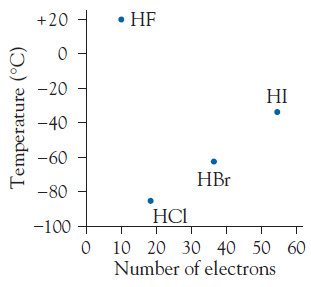
\includegraphics[width=\columnwidth]{Atom-ogMolekylefysik/billeder/HX-kogepunkt.png}
	\caption{Kogepunkterne for hydrogenhaliderne.} %Kilde: DIC.}
	\label{fig:HX-kogepunkt}
\end{figure}
\begin{opgave}{Halogener og hydrogenbindinger}{3}
Et vigtigt resultat der lægger grunden for en masse kemi, er at elektronkonfigurationer, hvor den yderste $s$- og $p$-orbital er fyldte er særligt stabile, hvilket leder til, hvad der i kemi kaldes "oktetreglen". Dette resultat har nogle interessante konsekvenser, der her vil undersøges.
\opg Hvilken elektronkonfiguration har flour, $F$, der er grundstof nummer 9?
\opg Flour står i 17. gruppe, der også kaldes halogenerne, som alle er karakteriseret ved at have samme elektronkonfiguration i deres yderste $s$- og $p$-orbitaler. Hvorfor er denne konfiguration speciel?
\opg Ligesom hydrogen samler halogenerne sig i molekyler på formen $\mathrm{X}_2$, hvor X er et vilkårlig halogen. Blandes en halogengas med hydrogengas forekommer følgende reaktion
\begin{align*}
	\mathrm{H}_2(g) + \mathrm{X}_2(g) \rightarrow 2 \mathrm{HX}(g)
\end{align*}
Forklar med et molekylorbitaldiagram, hvorfor HF er mere stabilt end $\mathrm{H}_2$ og $\mathrm{F}_2$.
\opg Hvilke atomorbitaler danner bindingen i HF, og hvilken type er det?
\opg I eksemplet med $\mathrm{H}_2$ er de to atomer ens, hvorfor orbitalen er symmetrisk omkring en akse midt imellem de to atomer. Hvis de to atomer er forskellige, eller det ikke er samme orbitaler der binder, er dette ikke nødvendigvis sandt. Hvorfor er molekylorbitalen for HF forskudt og imod hvilket atom?
\opg Denne forskydning giver HF et dipolmoment\footnote{Mere præcist kan det siges, at der er størst sandsynlighed for at de bindende elektroner befinder sig tættere på det ene atom end det andet, og ikke omvendt eller ligeligt fordelt. Det betyder at forventningsværdien, $\expect{\v{r}}$, vil være forskudt mod det ene atom. Det siges derfor ladningen i gennemsnit samler sig hos dette atom, som så er partielt negativt ladet, mens det andet er partielt positivt ladet.}, hvilket i denne sammenhæng fint kan tænkes som en ladningsforskydning, hvor alle elektronerne befinder sig tættere på det ene atom end det andet. Forklar hvorfor det betyder, at et HF-molekyle tiltrækkes af de andre, hvilket kaldes at de danner hydrogenbindinger?
\opg HF er det eneste af hydrogenhaliderne, HX, der kan danne hydrogenbindinger, hvilket kan ses på deres kogepunkter, figur \ref{fig:HX-kogepunkt}. Hvorfor det? \\ \\
Netop denne forskel gør flussyre, der er en vandig opløsning af HF, speciel. Den er i modsætning til de andre hydrogenhalider i stand til at opløse glas, hvorfor den ikke er så let at opbevare. Derudover kan den trænge igennem huden og opløse kroppen indefra, hvorfor eksempelvis saltsyre, HCl, oftere benyttes i laboratoriet.
\end{opgave}
\section*{Spin}
\begin{opgave}{Pauli princippet uden spin}{1}
Lad $\op O$ være ombytningsoperatoren. Som navnet antyder er det den operator, der får to elektroner til at bytte plads:
$$
\op O \Psi(x_1,x_2) = \Psi(x_2,x_1)
$$
Lad $\psi(x)$ være en én elektron tilstand, og $\Psi(x_1,x_2) = \psi(x_1)\psi(x_2)$.
\opg Hvad er $\op \Psi(x_1,x_2)$?\\
For at en tilstand kan opfylde Pauli princippet, skal bølgefunktionen være antisymmetrisk under ombytning. Det vil sige $\Psi(x_1,x_2) = -\Psi(x_2,x_1)$.
\opg Er $\Psi(x_1,x_2)$ tilladt ifølge Pauli?
\end{opgave}
%
\begin{opgave}{Rumbølgefinktioner}{2}
Lad os i stedet se på to elektroner i to forskellige tilstande $\psi_1$ og $\psi_2$. Her indikerer subscriptet på $\psi$ tilstanden, men subscripts på $x$ angiver hhv. elektron 1 og 2.\\
Lad nu
\begin{align*}
\Psi_{12}(x_1,x_2) &= \psi_1(x_1)\psi_2(x_2) \, , \\
\Psi_{21}(x_1,x_2) &= \psi_2(x_1)\psi_1(x_2) \, .
\end{align*}
Udregn de følgende ombytninger.
\opg $\op O \Psi_{12}(x_1,x_2)$.
\opg $\op O \Psi_{21}(x_1,x_2)$.
\opg $\op O \Psi^S(x_1,x_2)=\op O (\Psi_{12}(x_1,x_2)+\Psi_{21}(x_1,x_2))$.
\opg $\op O \Psi^A(x_1,x_2)=\op O (\Psi_{12}(x_1,x_2)-\Psi_{21}(x_1,x_2))$.
\opg Er bølgefunktionerne symmetriske, antisymmetriske eller ingen af delene.
\end{opgave}
%
\begin{opgave}{Pauli med spin}{3}
Nu vil vi tage højde for spin. Det gøres ved at multiplicere bølgefunktionen med en spinfunktion. Elektronen kan have spin op eller spin ned. Det angives med $\alpha$ eller $\beta$. For at holde styr på hvilken partikel der har hvilket spin tilføjes et tal til spinfunktionen. Så har partikel 1 spin op og partikel 2 spin ned skrives det: $\chi=\alpha(1)\beta(2)$.
Ombytningsoperatoren ombytter også, hvilken partikel der har hvilket spin.
Hvad er:
\opg $\op O \alpha(1)\alpha(2)$.
\opg $\op O \beta(1)\beta(2)$.
\opg $\op O \alpha(1)\beta(2)$.
\opg $\op O \beta(1)\alpha(2)$.
\opg Brug dette til at finde tre spinfunktioner, der er symmetriske under ombytning.
\opg Find en spinfunktion der er antisymmetrisk under ombytning.\\ \\
Tag nu højde for både spin- og rumdelen af den totale bølgefunktion.
\opg Hvor mange muligheder er der, der er tilladt af Pauli princippet, når de to elektroner har samme tilstand?
\opg Hvad er denne tilstand?
\opg Hvor mange bølgefunktioner er tilladte, når de to elektrontilstande er forskellige.
\end{opgave}
\chapter{Planetbevægelse}
%
%
\section*{Planetbaner og excentricitet}
%
%
\begin{opgave}{Excentricitet og planetbaner}{1}
Betragt formlen for afstanden mellem to objekter i bane omkring hinanden, ligning \eqref{k-eq:Ellipse_i_polaere_koordinater} i kompendiet.
\opg Lad $\epsilon = 0$. Hvad er $r(\phi)$? Og hvilken geometrisk form er dette?
\opg Lad $\epsilon = 1$. Hvilket keglesnit fås? Hvad sker der med $r(\phi)$, når $\phi$ vokser mod $\pi$?
\opg Lad $\epsilon > 1$. Hvordan er dette tilfælde sammenlignet med det, hvor $\epsilon = 1$? Beskriv forskellene mellem disse to.\\
Hint: Undersøg grænsebetingelser.
\end{opgave}
%
%
\begin{opgave}{Halleys komet}{1} \label{opg:Halleys_komet}
Halleys komet, navngivet efter den angelske astronom Edmund Halley, kredser om Solen i en meget elliptiske bane med $\epsilon = 0,967$. Den korteste afstand, som kommeten har til Solen, er $0,59 \, \text{AU}$.
%
\opg Opstil et udtryk for den største afstand $r_{\mathrm{maks}}$ som funktion af den korteste afstand $r_{\mathrm{min}}$.
%
\opg Beregn den største afstand til Solen.\\ \\
\end{opgave}
%
%
\begin{opgave}{Excentricitet}{1}
\opg Find et udtryk for excentricitetet fra formlen udledt i opgave \ref{opg:Halleys_komet}.
%
\opg Hvad er den største og mindste værdi, som excentriciteten kan antage? Hvilke(n) type(r) bane(r) gør dette sig gældende for, og hvorfor?
\end{opgave}
%
%
%
\section*{Tolegemeproblemet}
%
%
\begin{opgave}{Ækvivalens i tolegemeproblemet}{1} \label{opg:AekvivalensITolegemeproblemet}
I beskrivelsen af tolegemeproblemet blev det konkluderet, at den fælles afstand $r(\phi)$ mellem de to objekter, kan beskrives som en ellipse, der er en funktion af vinklen $\phi$ med brændpunkt i origo. Hvis vi kigger på et system bestående kun af Jorden og Solen, så betyder dette resultat, at det er lige så gyldigt at lægge solen i brændpunktet og se Jordens ellipsebevægelse omkring Solen, som at gøre det den anden vej rundt. Hvis Jorden lægges i brændpunktet, således at Jorden sættes til at stå stille, og Solens ellipsebane omkring Jorden observeres, hvordan vil massemidtpunktet så bevæge sig rent symbolsk?
\end{opgave}
%
%
\begin{opgave}{Ækvivalens i tolegemeproblemet II}{1}
I opgave \ref{opg:AekvivalensITolegemeproblemet} blev Jorden sat som at være i brændpunktet. I denne opgave sættes massemidtpunktet i stedet i brændpunktet. Må man dette, og hvis ja, hvorfor? Hvordan vil Jordens og Solens bevægelse i dette tilfælde se ud?
\end{opgave}
%
%
%
\section*{Bevægelsesligningerne}
%
%
\begin{opgave}{Bevarelse af impulsmoment}{1} \label{opg:Bevarelse_af_impulsmoment}
I afsnittet om bevarelse af impulsmoment i kompendiet argumenterede vi for, at det samlede impulsmoment for tolegemesystemet er bevaret.\\
I denne opgave skal det samme vises, men denne gang med udgangspunkt i hvert af legemerne for sig.
%
\opg Lad origo være i massemidtpunktet for tolegemesystemet og tegn dette system, hvor legemerne (kaldet 1 og 2) er i apoapsis af deres bane, og indtegn disse baner, når der tages højde for deres relative excentricitet. Angiv også stedvektorerne for de to legemer. Tegn gerne stort, da der i senere spørgsmål skal tilføjes til denne tegning.
%
\opg Indtegn de virkende kræfter og tag højde for deres relative længder.\\[2.5mm]
%
Fra kapitlet om dynamik af roterende legemer i Analytisk Mekanik, udledte vi en ligning for kraftmomentet på et legeme, ligning \eqref{k-eq:Kraftmoment}
\begin{align*}
	\v{\tau} &= \v{r} \times \v{F} \: ,
\end{align*}
og for impulsmomentet, ligning \eqref{k-eq:L}
\begin{align*}
	\v{\ell} &= \v{r} \times \v{p} \: .
\end{align*}
%
\opg Beregn kraftmomentet for hvert af legemerne.
%
\opg Hvad fortæller de beregnede kraftmomenter om impulsmomenterne? Og hvad kan der herudfra konkluderes om systemets totale impulsmoment?
%
\opg Indtegn retningen af det totale impulsmoment på tegningen, idet hvert af legemerne bevæger sig mod uret i deres respektive baner.
\end{opgave}
%
%
\begin{figure}[h!]
	\centering
	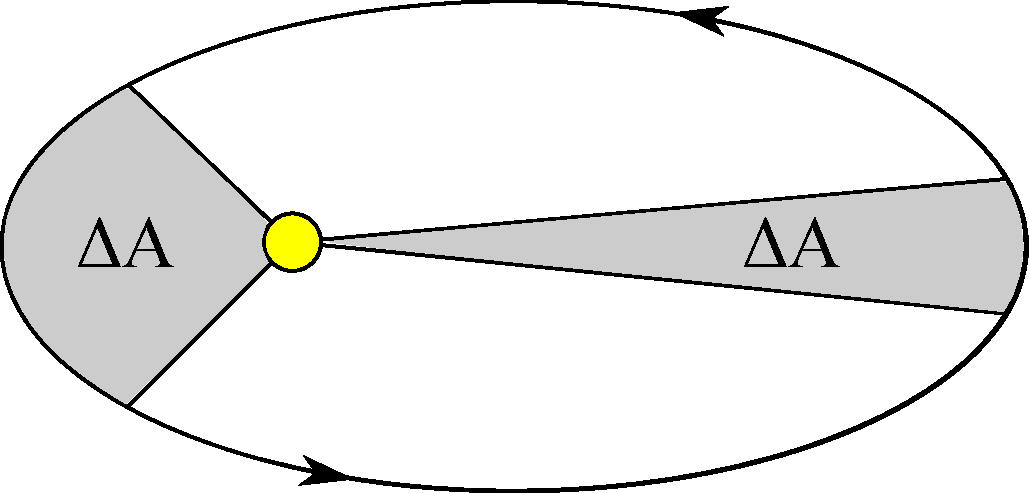
\includegraphics[width=\columnwidth]{Planetbevaegelse/Kepler2.pdf}
	\caption{Keplers 2. lov: I lige store tidsrum $\Delta t$ overstryger linjen mellem planeten og stjernen lige store arealer $\Delta A$.}
	\label{fig:Kepler2}
\end{figure}
%
\begin{opgave}{Keplers 3. lov}{2}
Keplers 2. lov beskriver, at en planet bevæger sig i sin bane, således at linjen fra stjernen til planeten, som kredser om denne, overstryger lige store arealer i lige store tidsrum, se figur \ref{fig:Kepler2}. Raten som linjen overstryger arealet med er dermed konstant, og den er givet ved
\begin{align*}
	\dif{t}{A} &= \frac{\ell}{2\mu} \: ,
\end{align*}
hvor $\ell$ er impulsmomentet og $\mu$ er den reducerede masse. Det totale areal for en ellipse er givet ved
\begin{align*}
	A &= \pi a b \: ,
\end{align*}
hvor $a$ og $b$ er hhv. den halve stor- og lilleakse.\\
Perioden for planeten er givet ved
\begin{align*}
	P &= \frac{A}{\d A / \d t} \: .
\end{align*}
%
\opg Udled ved hjælp af ovenstående og nogle formler fra kompendiet Keplers 3. lov:
\begin{align*}
	P^2 &= \frac{4\pi}{G(m_1+m_2)}a^3 \: .
\end{align*}
\end{opgave}
%
%
\begin{opgave}{Energibevarelse og excentricitet}{3}
For at finde en sammenhæng mellem excentricitet og energi betragtes en komet, der bevæger sig omkring et større objekt. Husk at energien, kompendiets ligning \eqref{k-eq:Bevaegelsesligningerne_energi}, er giver ved
\begin{align*}
	E &= \frac{1}{2}\mu v^2 + V_{\text{eff}}(r) \: .
\end{align*}
I opgaven anvendes det at
\begin{align*}
	V_{\text{eff}}(r) &= \frac{\ell^2}{2\mu r^2}-\frac{\gamma}{r} \: ,
\end{align*}
hvor $\gamma = Gm_1m_2$.
%
\opg Hvad vil kometens hastighed være, når den er tættest på objektet, altså i en afstand $r_{min}$ fra det? Og hvad vil energien så være i dette tilfælde?\\
Hint: Til at bestemme hastigheden, prøv at overvej hvilken retning, den vil have lige før $r_{min}$ samt lige efter. Husk at der kigges på et endimensionelt problem. Overvej at tegne $r$ som funktion af vinklen.
%
\opg Beregn $r_{\text{min}}$. Anvend definitionen af konstanten
\begin{align*}
	c = \frac{\ell^2}{\gamma\mu} \: .
\end{align*}
%
\opg Indsæt værdien for $r_{\text{min}}$ i udtrykket for energie, $E(r_{\text{min}})$, og bestem et udtryk for energien ud fra excentriciteten. Anvend energibevarelse til at bestemme energien til alle steder på kometens bane.
%
\opg Relater resultatet til de mulige baner. Hvis kometens totale energi er negativ, hvilken excentricitet kræves der så? Og hvordan bliver banen så? Hvad hvis energien er $0$? Eller hvis den er positiv?
\end{opgave}
%
%
%
\section*{Baneskift}
%
%
\begin{opgave}{Boostfaktor}{1}
En satellit er i kredsløb om Jorden i en cirkulær bane. Tegn den bane som fremkommer, når
\opg $\lambda > 1$.
\opg $1 > \lambda > 0$.
\opg $0 > \lambda > -1$.
\opg $\lambda < -1$.
\end{opgave}
%
%
\begin{opgave}{Boostkraft}{2}
En satellit boostes i punktet $P$ med en boostfaktor $\lambda$ for at skifte mellem to baner.
%
\opg Vis at det tidslige gennemsnit af en kraft er givet ved
\begin{align*}
	\v{F}_{av} &= \frac{\Delta \v{p}}{\Delta t} \: .
\end{align*}
%
\opg Find størrelsen af boostkraften som satellitten skal påvirkes med i løbet af boostet, som foregår over et kort tidsrum $\Delta t$.\\
Hint: Brug forskellen i impulsmoment til at finde forskellen i impuls i punktet $P$.
\end{opgave}
%
%
\begin{opgave}{Hohmannbane}{2} \label{opg:Hohmannbane}
En måde at lave et baneskift er ved brug af en Hohmannbane. Denne bane er en ellipse, som har periapsis i den ene bane og apoapsis i den anden.\\
I denne opgave betragtes en satellit, der benytter en Hohmannbane til at skifte mellem to cirkulære baner, figur \ref{fig:Hohmann}, med radius $R_1$ og $R_3 = 2R_1$.
%
\opg I hvilket punkt, $P$ eller $P'$, har Hohmann-banen hhv. periapsis og apoapsis.
%
\opg Beregn boostfaktoren $\lambda$ for satellittens boost ved punktet $P$.\\
Hint: Opstil et udtryk for $R_3$ ved $R_1$.\\
%
\opg Beregn boostfaktoren $\lambda'$ for satellittens boost ved punktet $P'$.\\
Hint: Betragt sammenfaldet mellem de to baner i $P'$.
%
\opg Brug impulsmomentbevarelse til at udtrykke satelittens hastighed $v_3$ efter begge boosts ved dens hastighed $v_1$ før boostene.
\end{opgave}
%
%
\begin{figure}[h!]
	\centering
	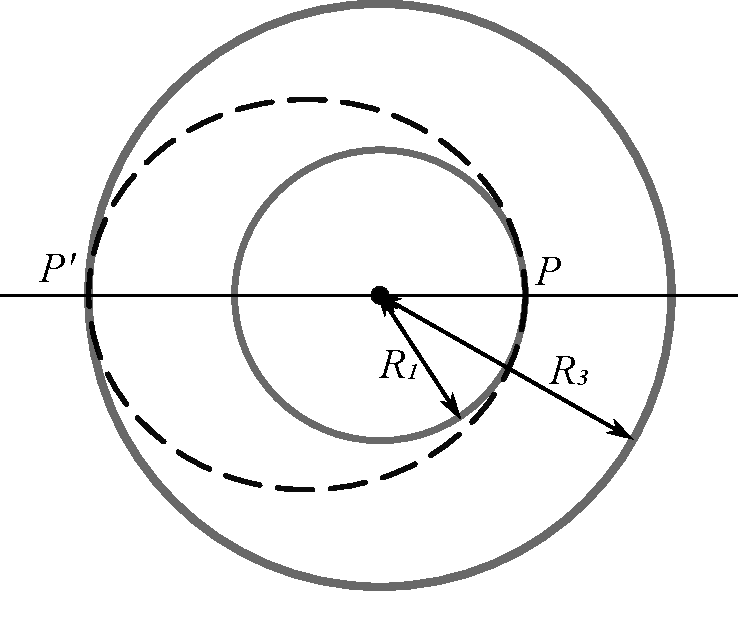
\includegraphics[width=\columnwidth]{Planetbevaegelse/Hohmann.pdf}
	\caption{To cirkulære baner (grå) og en Hohmannbane (stiplet) til at skifte mellem banerne.}
	\label{fig:Hohmann}
\end{figure}
%
%
\begin{opgave}{Hohmannbane II}{2}
En satellit vil nu gerne i to steps skifte mellem tre cirkulære baner. I første step skifter den fra bane A til C via Hohmannbanen 1, og i andet step skifter den fra bane C til bane B via Hohmannbanen 2. Se figur \ref{fig:Hohmann2}. Bane A har radius $R_A$, bane B har radius $R_B = 3R_A$ og bane C har radius $R_C = 1,5 R_B = 4,5 R_A$. Beregn følgende boostfaktorer.
%
\opg $\lambda_1$ i punktet $P$ for at skifte fra bane A til Hohmannbanen 1.
\opg $\lambda_1'$ i punktet $P'$ for at skifte fra Hohmannbanen 1 til bane C.
\opg $\lambda_2$ i punktet $Q$ for at skifte fra bane C til Hohmanbanen 2.
\opg $\lambda_2'$ i punktet $Q'$ for at skifte fra Hohmannbanen 2 til bane B.
%
\opg Hvad gør sig gældende for formen af boostfaktorerne $\lambda_1$ og $\lambda_2$ samt $\lambda_1'$ og $\lambda_2'$?\\
Hint: Generaliser boostfaktorerne.
\end{opgave}
%
\begin{figure}[h!]
	\centering
	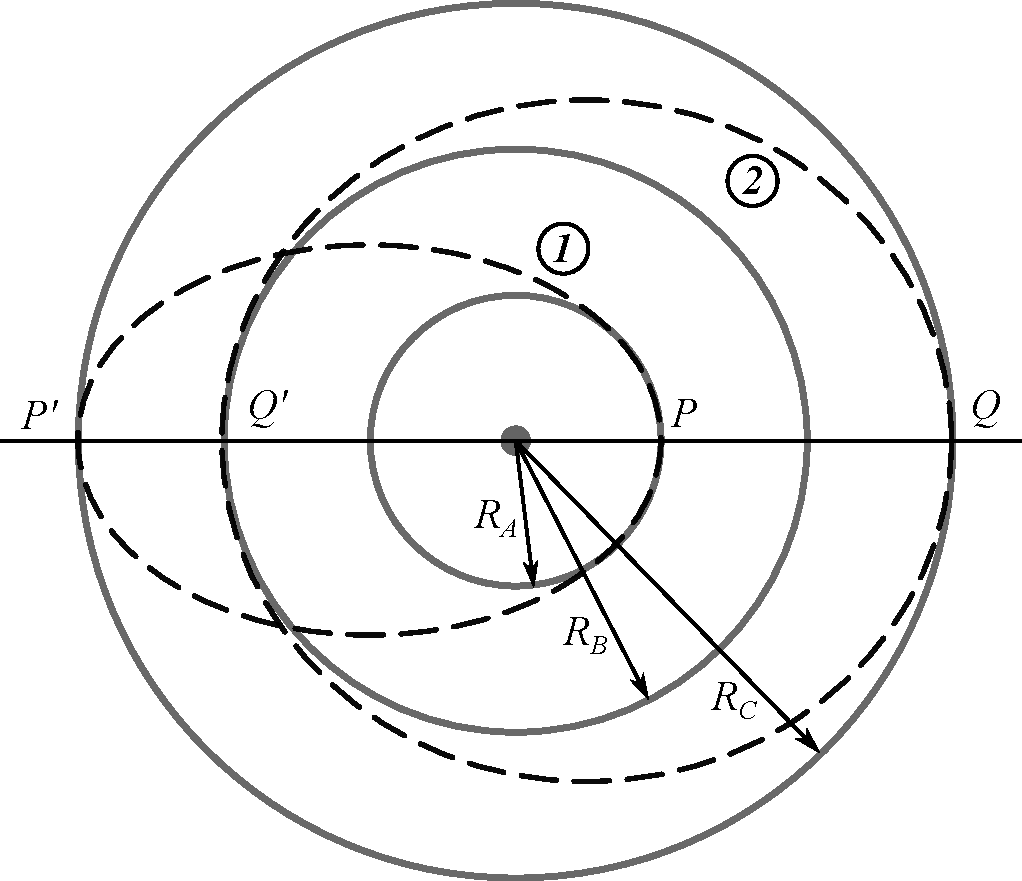
\includegraphics[width=\columnwidth]{Planetbevaegelse/Hohmann2.pdf}
	\caption{Tre cirkulære baner (grå) og to Hohmannbaner (stiplede) til at skifte mellem banerne.}
	\label{fig:Hohmann2}
\end{figure}
 


\onecolumn

\setlength{\tabcolsep}{1.5 em}
\def\arraystretch{1.35}

\newpage

\section{Nyttige fysiske konstanter og enheder}\label{mat:sec:fysiskekonstanter}

Her giver vi en tabel med nogle af de vigtige konstanter og enheder, som vi kommer til at bruge igennem de følgende kapitler. \\[5mm]

\vspace*{-\baselineskip}
\begin{table}[h!]
\centering
\begin{tabular}{llll}
%
%\multicolumn{4}{c}{\Large{\textbf{Fysiske Størrelser, Konstanter og Specielle Enheder}}} \\[2mm]
\hline
%
\textbf{Konstant} & \textbf{Symbol} & \textbf{Værdi} & \textbf{Enhed} \\ \hline
Lysets fart i vakuum & \si{\clight} & \num{2,99792458e8} & \si{\metre\per\second} \\
Gravitationskonstanten & $G$ & \num{6,6742e-11} & \si{\newton\metre\squared\per\kilo\gram\squared} \\
Plancks konstant & $h$ & \num{6,6260693e-34} & \si{\joule\second} \\
Reduceret Plancks konstant & $\hbar = \nicefrac{h}{2\pi}$ & \num{1,0545718e-34} & \si{\joule\second} \\
Boltzmanns konstant & $\kb$ & \num{1,3806506e-23} & \si{\joule\per\kelvin} \\
Stefan-Boltzmanns konstant & $\sigma$ & \num{5,670373e-8} & \si{\watt\per\metre\squared\per\kelvin\tothe4} \\
Avogadros tal & $N_A$ & \num{6.022141e23} & \si{\per\mole} \\
Gaskonstanten & $R=N_A\kb$ & \num{8.3144598} & \si{\joule\per\mole\per\kelvin} \\
Elementarladningen & $e$ & \num{1,602176565e-19} & \si{\coulomb} \\
Vakuumpermittiviteten & $\epsilon_0$ & \num{8,854187817e-12} & \si{\coulomb\squared\per\newton\per\metre\squared} \\
Vakuumpermeabiliteten & $\mu_0$ & \num{4\pi e-7} & \si{\newton\per\ampere\squared} \\[2mm] \hline
%
\textbf{Størrelse} & \textbf{Symbol} & \textbf{Værdi} & \textbf{Enhed} \\ \hline
%
Bohrradius & $a_0$ & \num{5,2917721067e-11} & \si{\metre} \\
%Jordens radius & $R_\oplus$ & \num{6,371e6} & \si{\metre} \\
%Jordens masse & $M_\oplus$ & \num{5,97219e24} & \si{\kilo\gram} \\
%Solens radius & $R_\odot$ & \num{6,95700e8} & \si{\metre} \\
%Solens masse & $M_\odot$ & \num{1,9891e30} & \si{\kilo\gram} \\
%Solens overfladetemperatur & $T_\odot$ & \num{5,778e3} & \si{\kelvin} \\
%Jupiters masse & $M_J = M_\mathrm{Jup}$ & \num{1.898e27} & \si{\kilo\gram} \\
Jordens radius & \si{\earthradius} & \num{6,371e6} & \si{\metre} \\
Jordens masse & \si{\earthmass} & \num{5,97219e24} & \si{\kilo\gram} \\
Solens radius & \si{\solarradius} & \num{6,95700e8} & \si{\metre} \\
Solens masse & \si{\solarmass} & \num{1,9891e30} & \si{\kilo\gram} \\
Solens overfladetemperatur & \si{\solartemperature} & \num{5,778e3} & \si{\kelvin} \\
Jupiters masse & $\si{\jupitermass} = \mathrm{M}_\mathrm{Jup}$ & \num{1.898e27} & \si{\kilo\gram} \\
Protonens masse & $m_p$ & \num{1,672621898e-27} & \si{\kilo\gram} \\
Neutronens masse & $m_n$ & \num{1,674927471e-27} & \si{\kilo\gram} \\
Elektronens masse & $m_e$ & \num{9,10938356e-31} & \si{\kilo\gram} \\[2mm] \hline
%
\textbf{Enhed} & \textbf{Symbol} & \textbf{Værdi} & \textbf{SI-Enhed} \\  \hline
%
Astronomisk enhed & \si{\astronomicalunit} & \num{1,49597870700e11} & \si{\metre} \\
Lysår & \si{\lightyear} & \num{9.4605284e15} & \si{\metre} \\
Parsec & \si{\parsec} & \num{3.08567758e16} & \si{\metre} \\
Atomar masseenhed & \si{u} & \num{1.66053904e-27} & \si{\kilo\gram} \\
Ångström & \si{\angstrom} & \num{1,0e-10} & \si{\metre} \\
Elektronvolt & \si{\electronvolt} & \num{1.60217662e-19} & \si{\joule} \\
År & \si{\year} & \num{31556925.445} & \si{\second} \\[.5mm] \hline
\end{tabular}
\end{table}

\addcontentsline{toc}{part}{Fysiske Størrelser, Konstanter og Specielle Enheder} % Tilføjer Fysiske_Konstanter.tex til toc som en "part"

\setcounter{chapter}{0} % Resets chapter numbers
\renewcommand{\theHchapter}{\Alph{chapter}} % Reset hyperlink references to chapters (for sections use "section" both places instead of "chapter", eg. "theHsection")

\part{Facitlister}
\chapter{Analytisk Mekanik}
%
%
\section*{Koordinatsystemer}
\begin{opgave}{Gode koordinatsystemer}{1}
\opg Det gode koordinatsystem beskriver et problem så simpelt som muligt, og det har det færrest mulige antal frihedsgrader.
\opg Symmetrier mindsker antallet af frihedsgrader, fordi det restringerer koordinaterne, således at et eller flere koordinater ophører med at være frie.
\opg Det simpleste er at bruge det koordinatsystem, som beskriver symmetrien bedst. \\
a) Kartesisk koordinatsystem, idet planer beskrives ved et fastholdt kartesisk koordinat. Eksempelvis er $xz$-planet alle punkter hvor $y=0$, men dette gælder også for ethvert andet plan i rummet. Bemærk også at $xy$-planet er lige simpelt beskrevet i cylinderkoordinater. \\
b) Cylindrer er pænest beskrevet i cylinderkoordinater, hvorfor dette er det smarte valg, se opgave \ref{opg:Cylinder}. \\
c) Sfærer er simplest i sfæriske koordinater, hvorfor det er lettest at bruge sfæriske koordinater. Sfærisk symmetri ser man ofte i problemer hvor det er afstanden mellem to objekter, der er afgørende, for eksempel den gravitationelle interaktion mellem to legemer.
\end{opgave}
%
%
\begin{opgave}{Generaliserede koordinater}{1}
\opg $r$ er afstanden fra centrum og $\phi$ er en vinkel der beskriver hvor på cirkelen objektet er. Her er valgt vinkelen fra vandret. Lidt trigonometri giver at $x$ og $y$ er:
\begin{align*}
	x &= r\cos(\phi)\\
	y &= r\sin(\phi)
\end{align*}
\opg Når objektet bevæger sig ændres både $x$ og $y$, hvorfor to koordinater ændres.
\opg Afstanden til centrum er altid den samme så $r=R$ altid.
\opg Da $R$ er konstant er det nok at beskrive systemet med vores ene variabel $\phi$.
\opg Vi vil gerne beskrive systemet så simpelt så muligt, derfor er det smartest at bruge polære koordinater.
\end{opgave}
%
%
\begin{figure}
	\centering
	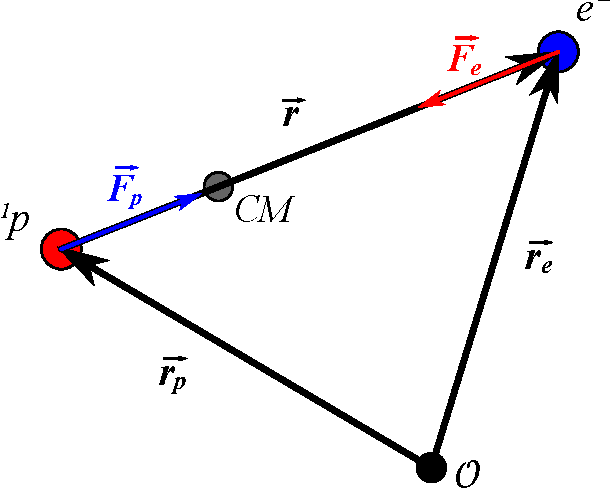
\includegraphics[width=.6\textwidth]{Analytisk-Mekanik/Brint.pdf}
	\caption{Illustration af brintatomet med arbitrært origo, $\mathcal{O}$, og massemidtpunkt $CM$. Derudover er kraften fra protonen på elektronen, $\v{F}_e$, indtegnet og farvet rød for at gøre den tydeligere, og ligeså for den blå kraft fra elektronen på protonen.}
	\label{fig:Brint}
\end{figure}
%
%
\begin{opgave}{Brint}{2}
\opg Eftersom $m_p\approx2000m_e$ er massemidtpunktet forskudt mod protonen således at at $\v{r}_e$ er i størrelsesordenen $2000\v{r}_p$. For at gøre tegningen overskuelig er massemidtpunktet angivet markant tættere på midten, se figur \ref{fig:Brint}.
\opg Afstanden mellem protonen og elektronen.
\opg Se figur \ref{fig:Brint}.
\opg I massemidtpunktet, da problemet så reducerer til to generaliserede koordinater, idet der altid eksisterer en linje, som både protonen, elektronen og deres fælles massemidtpunkt befinder sig på.
\opg Antagelsen giver mulighed for at benytte følgende approksimationer
\begin{align*}
	&a) \quad m_p + m_e \simeq m_p \: , \\
	&b) \quad \frac{m_e}{m_p} \simeq 0 \: ,
\end{align*}
hvorved
\begin{align*}
	\v{r}_\textsc{cm} &= \frac{m_e\v{r}_e + m_p\v{r}_p}{m_e + m_p} \\
	&\simeq \frac{m_e\v{r}_e + m_p\v{r}_p}{m_p} \\
	&= \frac{m_e}{m_p}\v{r}_e + \v{r}_p \\
	&\simeq \v{r}_p \: .
\end{align*}
\opg $\v{F} = -\dfrac{e^2}{4\pi\epsilon_0}\dfrac{\v{r}_e}{r_e^3}$ idet $\v{r}_p = 0$ i dette koordinatsystem.
\end{opgave}
%
%
\section*{Energi}
%
%
\begin{opgave}{Energibevarelse}{1}
\opg Det kunne være nogle af følgende: \\
-- \: Kinetisk energi \\
-- \: Potentiel energi \\
-- \: Mekanisk energi \\
-- \: Termisk energi \\
-- \: Elektrisk energi \\
-- \: Kemisk energi \\
-- \: Bindingsenergi \\
-- \: Masse \\
-- \: Et cetera
\opg Der er flere mulige forklaringer, men her er nogle forslag: \\
-- \: En konservativ kraft er en kraft for hvilken arbejdet, den udfører, på et legeme under bevægelse fra et punkt til et andet, er uafhængig af vejen mellem de to punkter. \\
-- \: En konservativ kraft er en kraft, der omsætter potentiel energi til kinetisk energi eller omvendt uden tab. \\
-- \: En konservativ kraft er en kraft, der bevarer mekanisk energi. \\
-- \: Hvis et legeme bevæger sig i en lukket bane og det totale arbejde fra en kraft et nul, da siges kraften at være konservativ.\\ 
-- \: $\v{F}$ er konservativ, hvis
\begin{align*}
	\oint\v{F}\cdot\d\v{l} = 0
\end{align*}
-- \: En konservativ kraft er udelukkende stedafhængig, og ethvert punkt i rummet kan derfor tildeles en potentiel energi.
\opg Der er flere muligheder her. Til bevaret mekanisk energi kan det eksempelvis være: \\
-- \: Bold i tyngdefelt i vakuum. \\
-- \: Lod på fjeder, uden gnidning, små udsving. \\
-- \: To ladede partikler. \\ \\
Tre situationer, hvor mekanisk energi ikke er bevaret, kan eksempelvis være: \\
-- \: Kugle skudt afsted under vand. \\
-- \: Deformation af fjeder/andet materiale, over elastisk grænse. \\
-- \: Uelastiske stød.
\opg I de tre foreslåede eksempler: \\
-- \: Kuglen påvirkes af vandmodstand. \\
-- \: Der går energi til deformation af fjederen. \\
-- \: Der går energi til deformation/sammensætning af de stødende legemer.
\end{opgave}
%
%
\begin{figure}
	\centering
	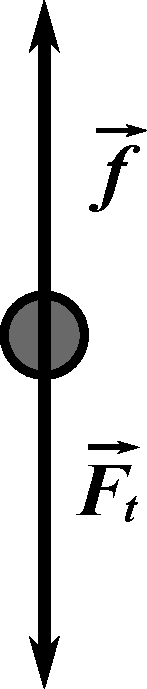
\includegraphics[width=.08\textwidth]{Analytisk-Mekanik/FritFald.pdf}
	\caption{Legemet er påvirket at en tyngdekraft $\v{F}_t$ og en friktionskraft $\v{f}$.}
	\label{fig:FritFald}
\end{figure}
%
%
\begin{opgave}{Frit fald}{1}
\opg Se figur \ref{fig:FritFald}.
\opg Friktion er ikke en konservativ kraft, idet den omsætter kinetisk energi til termisk energi i stedet for potentiel energi.
\opg Negliceres friktion er der energibevarelse, hvorfor
\begin{align*}
	\frac{1}{2}mv_0^2 + mgh &= \frac{1}{2}mv^2 + mg(0) \\
	\xRightarrow{v_0=0} mgh = \frac{1}{2}mv^2 \\
	v = \sqrt{2gh}
\end{align*}
\opg Hvis $h$ er meget stor er den en dårlig antagelse, idet legemet vil nå sin terminalhastighed, før den rammer Jorden. Negligeres friktionen ophører terminalhastigheden med at eksistere, hvilket gør antagelsen dårlig. \\
Luftmodstand beskrives ofte på en af de to følgende former:
\begin{align*}
	\v{f} =
		\begin{cases}
			-c_1v \\
			-c_2v^2
		\end{cases}
\end{align*}
hvor $v$ er hastigheden og $c_i$ er konstanter, som afhænger af legemets udformning. For at friktionskraften skal være negligibel, må konstanterne $c_i$ være relativt små, og $h$ skal være tilpas lille til at hastigheden ikke når at blive for stor, hvorfor et bud på et sæt af kriterier er
\begin{align*}
	h &\ll 2g \: ,\\
	c_i &< 1 \: .
\end{align*}
Der er ikke noget entydigt rigtigt svar, da problemet ikke skal analyseres grundigt nok til at gøre dette stringent, men der bør fremgå en fysisk forståelse for situationen af kriteriet.
\end{opgave}
%
%
\begin{opgave}{Kollisioner}{1}
\opg Newtons 3. lov.
\opg Newtons 3. lov giver at kraften er lige stor og modsatrettet.
\opg Af det ovenstående er
\begin{align*}
	\v{F}_1 = -\v{F}_2 \: ,
\end{align*}
hvorved Newtons 2. lov siger at den samlede kraft på systemet er
\begin{align*}
	\v{F}_1 + \v{F}_2 &= \dif{t}{}(\v{p}_1 + \v{p}_2) \\
	\v{F}_1 - \v{F}_1 &= \dif{t}{}(\v{p}_1 + \v{p}_2) \\
	0 &= \dif{t}{}(\v{p}_1 + \v{p}_2) \: .
\end{align*}
Ergo er den totale impuls bevaret.
\opg Af opgave \ref{opg:Energibevarelse} er et legemes mekaniske energi bevaret, hvis legemet kun er påvirket af konservative kræfter. Da der er set bort fra eventuelle ydre kræfter, er den potentielle energi i systemet $V=0$, hvorfor den kinetiske energi er bevaret, hvis legemerne kun påvirker hinanden med konservative kræfter. \\
a) Af definitionen af et elastisk stød, er legemerne kun påvirket af konservative kræfter, hvorfor den kinetiske energi er bevaret. \\
b) Uelastiske kollisioner er alle kollisioner, hvor legemerne påvirker hinanden på en måde, der er ikke er konservativ, hvorfor den kinetiske energi ikke er bevaret.
\end{opgave}
%
%
\begin{opgave}{Bevægelse omkring ligevægt}{2}
\opg $\dif{r}{V} = V_0\left(\frac{1}{R} - \lambda^2\frac{R}{r^2}\right)$
\opg Ligevægtspunktet bestemmes ved at sætte den afledede til nul og benytte nulreglen:
\begin{align*}
	0 &= \dif{r}{V} \: , \\
	\implies \frac{1}{R} &= \lambda^2\frac{R}{r^2} \: , \\
	\implies r_0 &= \lambda R \: .
\end{align*}
\opg Den andenafledte er:
\begin{align*}
	\dif[2]{r}{V} = \frac{2V_0R\lambda^2}{r^3} \: .
\end{align*}
\opg Der er tale om et minimum, hvis den anden afledede evalueret i minimaet er positiv. Det gælder da alle konstanterne er antaget positive.
\begin{align*}
	\left.\dif[2]{r}{V}\right|_{r = \lambda R} = \left.\frac{2V_0R\lambda^2}{r^3}\right|_{r = \lambda R} = \frac{2V_0}{\lambda R^2} > 0 \: .
\end{align*}
\opg Først isoleres $r$ i definitionen af $x$ og derefter indsættes det i funktionen $V(r)$.
\begin{align*}
	r &= x + r_0 \\
	\implies V(x) &= V_0\left(\frac{x + r_0}{R} + \lambda^2\frac{R}{x + r_0}\right)
\end{align*}
\opg Taylorudviklingen af en funktion $f(x)$ omkring $x=0$ til anden orden er
\begin{align*}
	f(x) \simeq f(0) + x\left.\dif{x}{f(x)}\right|_{x=0} + x^2\left.\frac{1}{2}\dif[2]{x}{f(x)}\right|_{x=0} \: .
\end{align*}
I første omgang bestemmes potentialets minimum
\begin{align*}
	V(x=0) &= V_0\left(\frac{\lambda R}{R} + \lambda^2\frac{R}{\lambda R}\right) \\
	&= 2V_0\lambda \: .
\end{align*}
Herefter bestemmes den første afledede evaluerede i nul
\begin{align*}
	 \left.\dif{x}{f(x)}\right|_{x=0} &= \left[\frac{V_0}{R} - V_0\lambda^2\frac{R}{(x+r_0)^2}\right]_{x=0} \\
	 &= \frac{V_0}{R} - V_0\lambda^2\frac{R}{r_0^2} \\
	 &= \frac{V_0}{R} - V_0\lambda^2\frac{R}{(\lambda R)^2} \\
	 &= \frac{V_0}{R} - \frac{V_0}{R} = 0 \: .
\end{align*}
Så den anden afledede
\begin{align*}
	 \left.\dif[2]{x}{f(x)}\right|_{x=0} &= \left[\dif{x}{f(x)}\left(\frac{V_0}{R} - V_0\lambda^2\frac{R}{(x+r_0)^2}\right)\right]_{x=0} \\
	 &= \left.\frac{2V_0R\lambda^2}{(x+r_0)^3}\right|_{x=0} \\
	 &= \frac{2V_0Rr_0\lambda^2}{r_0^3} \\
	 &= \frac{2V_0R\lambda^2}{(R\lambda)^3} \\
	 &= \frac{2V_0}{\lambda R^2} \: .
\end{align*}
Dermed bliver den potentielle energi omkring ligevægtspunktet $r_0$
\begin{align*}
	V(x) \simeq 2V_0\lambda + \frac{1}{2}\frac{2V_0}{\lambda R^2}x^2 = c + \frac{1}{2}kx^2 \: ,
\end{align*}
hvor $c$ og $k$ er defineret som
\begin{align*}
	c &= 2V_0\lambda \: ,\\
	k &= \frac{2V_0}{\lambda R^2} \: .
\end{align*}
Supplerende kan de siges at nulpunktet for potentiel energi er arbitrært, hvorfor $V = (1/2)kx^2$ er lige så validt et potential at benytte.
\opg Vinkelfrekvensen for den harmoniske oscillator er
\begin{align*}
	\omega = \sqrt{\frac{k}{m}} = \left(\frac{2V_0}{m\lambda R^2}\right)^{1/2} \: .
\end{align*}
Er det ikke oplagt at vinkelfrekvensen for en harmonisk oscillator opfylder at $\omega^2 = k/m$, så kan der henvises til de forskellige beskrivelser af pendulet, det vil sige afsnittene \ref{k-sec: Beskrivelse af pendul - Newton} og \ref{k-sec:PendulLagrange} i kompendiet.
\end{opgave}
%
%
\begin{opgave}{(Næsten) alt er en harmonisk oscillator}{3}
\opg Potentialet er arbitrært, så det indsættes bare i ligning \eqref{k-Taylor_pol} i kompendiet analogt til eksemplet med $e^x$
\begin{align} \label{eq:VTaylor}
	V(x) \simeq V(x=0) &+ x\left.\dif{x}{V(x)}\right|_{x=0} + \frac{1}{2}x^2\left.\dif[2]{x}{V(x)}\right|_{x=0} \: .
\end{align}
Der kan ikke gøres mere, da $V(x)$ er ukendt.
\opg Sammenlignes ligning \eqref{eq:VTaylor} med med den harmoniske oscillator, $f(x)$, i opgaven, ses det at
\begin{align*}
	c &= V(x=0) \: , \\[.5em]
	k &= \left.\dif[2]{x}{V(x)}\right|_{x=0} \: ,
\end{align*}
idet de afledede bliver en konstant, når de evalueres i et punkt. Ledet $x\left.\dif{x}{V(x)}\right|_{x=0}$ passer dog ikke ind, og kriteriet må derfor være at dette er nul for alle værdier af $x$, hvorfor differentialet må være nul:
\begin{align*}
	\left.\dif{x}{V(x)}\right|_{x=0} = 0 \enspace\forall \; x \Rightarrow \dif{x}{V(x)} = 0 \: .
\end{align*}
\opg Det kunne være følgende funktioner, hvor store bogstaver er konstanter
\begingroup
\allowdisplaybreaks
\begin{align*}
	\text{Parabel uden førstegradsled:} \qquad
	&f(x) = A + Bx^2 \\
	\text{Gaussfunktion:} \qquad
	&f(x) = -Ae^{-Bx^2}\\
	\text{Cirkel:} \qquad
	&f(x) = \frac{\pm A}{\sqrt{1-x^2}}\\
	\text{Morsepotentiale:} \qquad
	&f(x) = A\left(1-e^{-Bx}\right)^2\\
	\text{Potentialet fra opgave \ref{mek:opg:equilibrium}:} \qquad
	&f(x) = A\left(\frac{x}{B}+C^2\frac{B}{x}\right)\\
	\text{Effektivt potentiale for planetbevægelse:} \qquad
	&f(x) = \frac{A}{x^2}-\frac{B}{x} \\
	\text{Trigonometrisk:} \qquad
	&f(x) = A\cos(Bx + C) + D \\
	\text{Hyperbolsk cosinus:} \qquad
	&f(x) = A\left(e^{(Bx)} + e^{(-Bx)}\right) = 2A\cosh(Bx) \\
	\text{Og så videre:} \qquad &f(x) = ... 
\end{align*}
\endgroup
Cosinus og den hyperbolske cosinus kræver dog at de evalueres i et punkt, hvor henholdsvis sinus og sinus hyperbolsk er nul. Dermed kan sinus (hyperbolsk) også bruges under samme betingelser.
\opg $V(x)$ og $\tilde{V}(x)$ opfører sig ens hvis deres afledede er ens
\begin{align*}
	\pdif{x}{\tilde{V}(x)} = \pdif{x}{V(x)} + \pdif{x}{\lambda} \xleq{\partial\lambda/\partial x = 0} \pdif{x}{V(x)} \: ,
\end{align*}
da $\lambda$ er en konstant.
\opg Eftersom $c$ er en konstant gælder det samme for den, som for $\lambda$, hvorfor den kan lægges til med modsat fortegn. Derfor vælges $\lambda = -c$, hvorved den harmoniske oscillators potentielle energi kan skrives som
\begin{align*}
	\tilde{V}(x) = V(x) - c = \frac{1}{2}kx^2 \: .
\end{align*}
\end{opgave}
%
%
\section*{Etlegemeproblemer}
%
%
\begin{opgave}{Partikel på en cylinder}{1}
\opg Siden partiklen er fastlåst på overfladen af cylinderen er $r$ koordinatet altid lig radien af cylinderen:
$$
	r = R
$$
Resten er frie.
\opg Lad os starte med den letteste: $z$. Der er det samme i kartesiske og cylindriske koordinater.
$$
	\dt z = \dt z
$$
De to andre afhænger kun af $\phi$, så efter kædereglen følger:
\begin{align*}
	\dt x &= -R\dt \phi \sin(\phi)\\
	\dt y &= R\dt \phi \cos(\phi)
\end{align*}
\opg I kartesiske koordinater er:
$$
v^2 = \dt x^2+\dt y^2 + \dt z^2
$$
Vi kan her bruge Pythagoras sætning for enhedstrekanten:
$$
	\cos^2(\phi)+\sin^2(\phi) = 1
$$
Så den kinetiske energi er:
\begin{align*}
	K &= \frac{1}{2}mv^2\\
	&= \frac{m}{2}(R^2\dt \phi^2\sin^2(\phi)+R^2\dt  \phi^2\cos^2(\phi)+\dt z^2)\\
	&= \frac{m}{2}(R^2\dt \phi^2+\dt z^2) \: .
\end{align*}
\opg Siden potentialet er nul er Lagrangefunktionen:
$$
	L = K = \frac{m}{2}(R^2\dt \phi^2+\dt z^2)
$$
\opg Generelt er en Euler-Lagrangeligning på formen:
$$
	\el{\dt q} = \pdif{q}{L}
$$
Igen lad os starte med $z$.
\begin{align*}
	\pdif{\dt z}L &= m\dt z\\
	\el{\dt z} &= m\ddt z\\
	\pdif{z}{L} &= 0
\end{align*}
Det giver Euler-Lagrangeligningen for $z$:
$$
	m\ddt z = 0
$$
Tilsvarende for $\phi$
\begin{align*}
	\pdif{\dt \phi}L &= mR^2\dt \phi\\
	\el{\dt \phi} &= mR^2\ddt \phi\\
	\pdif{\phi}{L} &= 0
\end{align*}
Det giver Euler-Lagrangeligningen for $\phi$:
$$
	mR^2\ddt \phi = 0
$$
Begge differentialligninger kan reduceres så vi ender med:
\begin{align*}
	\ddt z &= 0 \: ,\\
	\ddt \phi &= 0 \: .
\end{align*}
\opg Begge differentialligninger giver bevægelse med konstant hastighed. For $z$ er det konstant hastighed langs cylinderaksen. For $\phi$ er det cirkulær bevægelse omkring aksen. Kombineret giver det en spiralbevægelse. Som en bonus er løsningen til bevægelsesligningerne:
\begin{align*}
	z(t) &= v_z t+z_+0 \\
	\phi(t) &= \omega t + \phi_0 \\
	x(t) &= R\cos(\omega t+\phi_0) \\
	y(t) &= R\sin(\omega t + \phi_0)
\end{align*}
\end{opgave}
%
%
\begin{opgave}{Atwoods faldmaskine}{1}
\opg Snorlængden er konstant, og af tegningen, figur \ref{fig:Atwood}, fremgår det at længden af snoren kan udtrykkes som
\begin{align*}
	l = x + y + \pi R \: .
\end{align*}
Da $R$ og $l$ er konstanter kan $y$ udtrykkes ved $x$ som
\begin{align} \label{eq:xAtwood}
	y = l - x - \pi R \: .
\end{align}
\opg Differentieres \eqref{eq:xAtwood} med hensyn til tid fås
\begin{align} \label{eq:AtwoodFart}
	\dt{y} = -\dt{x} \: ,
\end{align}
idet $l,\pi,R$ er konstanter.
\opg Den potentielle energi findes ved at bruge formlen $V = mgh$ hvor $h$ er forskydningen fra nulpunktet. Hvert lod er forskudt henholdsvis $x$ og $y$ i negativ retning, hvorfor
\begin{align} \label{eq:VAtwood}
	V = -g(m_1x + m_2y) \: .
\end{align}
Dette skyldes at nulpunktet for den potentielle energi for hvert lod er valgt til henholdsvis $x=0$ og $y=0$. Den potentielle energi skal så falde, når for hvert lod skal så falde, når henholdsvis $x$ og $y$ bliver mindre, hvilket giver fortegnet i ligning \eqref{eq:VAtwood}. \\
Er man stor modstander af konceptet om negativ potentiel energi, så kan man definere nulpunktet i afstanden $H$ under faldmaskinen. Derved bliver den højde, $h$, der er relevant for den potentielle energi henholdsvis
\begin{align*}
	h_1 = H - x
\end{align*}
og
\begin{align*}
	h_2 = H - y \: ,
\end{align*}
hvor subscribtet angiver hvilket lod, der er tale om.
\opg For kinetisk energi kastes ind i formlen $K = \sum_i\frac{1}{2}m_iv_i^2$, så der fås
\begin{align*}
	K = \frac{1}{2}(m_1\dt{x}^2 + m_2\dt{y}^2) = \: .
\end{align*}
\opg Lagrangefunktionen er pr. definition $L = K - V$. Bruges dette samt ligninger \eqref{eq:xAtwood} og \eqref{eq:AtwoodFart} fås
\begin{align*}
	L &= K - V \\
	&= \frac{1}{2}(m_1\dt{x}^2 + m_2\dt{y}) - (-g)(m_1x + m_2y) \\
	&=  \frac{1}{2}(m_1\dt{x}^2 + m_2(-\dt{x})^2) + g\Big[m_1x + m_2(l - x - \pi R)\Big] \\
	&= \frac{1}{2}(m_1+m_2)\dt{x}^2 + g\Big[m_1x + m_2(l - x - \pi R)\Big] \: .
\end{align*}
Havde man placeret nulpunktet for den potentielle energi afstanden $H$ under faldmaskinen, ville Lagrangefunktionen blive
\begin{align*}
	L = \frac{1}{2}(m_1+m_2)\dt{x}^2 - g\Big[m_1(H-x) + m_2(H - l + x + \pi R)\Big] \: .
\end{align*}
Den eneste forskel på de to Lagrangefunktioner er konstanter, og de forsvinder alligevel ved differentiation. Dette bruger konceptet at enhver Langrangefunktion, der giver den rigtige bevægelse, er en gyldig Lagrangefunktion, hvilket opgave \ref{opg:HO} også illustrerer.
\opg For at benytter Euler-Lagrangeligninger skal følgende differentialer bruges
\begin{align} \label{eq:AtwoodEL}
	\pdif{x}{L} &= g(m_1 - m_2) \\
	\pdif{\dt{x}}{L} &= (m_1 + m_2)\dt{x} \\
	\el{\dt{x}} &= (m_1 + m_2)\ddt{x}
\end{align}
Bruges Euler-Lagrangeligningen, ligning \ref{k-Euler-Lagrange} i kompendiet, til at sætte første og sidste udtryk i ligning \eqref{eq:AtwoodEL} fås
\begin{align*}
	(m_1 + m_2)\ddt{x} &= g(m_1 - m_2) \\
	\ddt{x} &= g\frac{m_1 - m_2}{m_1 + m_2}
\end{align*}
\opg Både $g$ og $m_1+m_2$ er positive led, hvorfor fortegnet er bestemt af tælleren.
\begin{align*}
	m_1>m_2: \quad m_1-m_2>0 \implies \ddt{x}>0 \\
	m_2>m_1: \quad m_1-m_2<0 \implies \ddt{x}<0
\end{align*}
Dette stemmer overens med det forventede, idet $\ddt{x}>0$ betyder at accelereres i positiv $x$-retningen, hvilket betyder at $m_1$ falder ned, mens $m_2$ trækkes op. Dette sker lige netop når $m_1>m_2$, hvilket også giver fysisk mening, idet det tungeste lod burde falde ned, og trække det letteste med sig. Der gælder det omvendte, hvis $m_2>m_1$.
\opg Udføres integralet fås
\begin{align*}
	x(t) &= \iint a\d t \d t \\
	&= \int at + v_0 \d t \\
	&= \frac{1}{2}at^2 + v_0t + x_0 \\
	&= \frac{1}{2}g\frac{m_1 - m_2}{m_1 + m_2}t^2 + v_0t + x_0 \: .
\end{align*}
\end{opgave}
%
%
\begin{opgave}{Yoyo}{1}
De ligninger, der henvises til siger at
\begin{align*}
	K &= \frac{1}{2}mv_\textsc{cm}^2 + \frac{1}{2}I\omega^2 \: , \\
	v &= r\dt{\phi} = r\omega \: .
\end{align*}
\opg Fra opgaven er $v = v_\textsc{cm} = \dt{z}$  da yoyoen kun bevæger sig translatorisk i $z$-retningen. Kombineres alt dette med informationen om intertimomentet fås
\begin{align*}
	K &\xleq{v=r\omega} \frac{1}{2}mv_\textsc{cm}^2 + \frac{1}{2}I\left(\frac{v}{r}\right)^2 \\
	&\xleq{v=v_\textsc{cm}=\dt{z}} \frac{1}{2}m\dt{z}^2 + \frac{1}{2}I\left(\frac{\dt{z}}{r}\right)^2 \\
	&\xleq{I = \frac{1}{2}mR^2} \frac{1}{2}m\dt{z}^2 + \frac{1}{4}mR^2\left(\frac{\dt{z}}{r}\right)^2 \: .
\end{align*}
\opg Den potentielle gravitationelle energi er $V = mgh$, hvor $h$ er den afstanden til nulpunktet i tyngdekraftens retning. Defineres nulpunktet sådan at $V(z=0)=0$ er $z=-h$, fordi $V$ skal blive mindre, når $z$ bliver større, hvorved $V = -mgz$. Her kan igen gøres det samme med at definere $V(x) = 0$ til et sted langt nede, og dermed indføre en konstant i den potentielle energi, som senere forsvinder ved differentiation.
\opg Benyttes definitionen af Lagrangefunktionen inden der sættes udenfor parentes fås
\begin{align*}
	L &= K - V \\
	&= \frac{1}{2}m\dt{z}^2 + \frac{1}{4}mR^2\left(\frac{\dt{z}}{r}\right)^2 - (-mgz) \\
	&= \frac{1}{2}m\left[1 + \frac{1}{2}\left(\frac{R}{r}\right)^2\right]\dt{z}^2 + mgz \: .
\end{align*}
\opg De afledede af Lagrangefunktionen er
\begin{align*}
	\pdif{z}{L} &= mg \: ,\\
	\pdif{\dt{z}}{L} &= m\left[1 + \frac{1}{2}\left(\frac{R}{r}\right)^2\right]\dt{z} \: , \\
	\el{\dt{z}} &= m\left[1 + \frac{1}{2}\left(\frac{R}{r}\right)^2\right]\ddt{z} \: .
\end{align*}
\opg Euler-Lagrangeligningen siger at det første og sidste differentiale er lig hinanden\footnote{Lighedstegnet vendes om tilsidst, da det ser pænest ud.}
\begin{align*}
	\pdif{z}{L} &= \el{\dt{z}}\\
	mg &= m\left[1 + \frac{1}{2}\left(\frac{R}{r}\right)^2\right]\ddt{z} \\
	g &= \left[1 + \frac{1}{2}\left(\frac{R}{r}\right)^2\right]\ddt{z} \\
	\ddt{z} &= \frac{g}{1 + \frac{1}{2}\left(\frac{R}{r}\right)^2} \: .
\end{align*}
\opg Med Newtonsk mekanik ville man være nød til at bestemme summen af kræfter og summen af kraftmomenter, der begge vil afhænge af snorkraften i snoren, $S$. Denne er ukendt, og derfor besværlig at regne med. Derudover ville man skulle bruge både Newtons 2. lov og Newtons 2. lov for roterende bevægelse, og så kæde det sammen gennem den ukendte snorkraft, hvilket er ret så omstændigt, sammenlignet med hvor elegant det er at benytte Lagrangemekanikken.
\end{opgave}
%
%
\begin{opgave}{Klods på en fjeder}{2}
Lagrangeformalismen bygger på systemets energier, hvorfor disse bestemmes først
\begin{align*}
	K &= \frac{1}{2}m\dt{x}^2 \\
	V &= \frac{1}{2}kx^2 \: .
\end{align*}
\opg Dermed bliver Lagrangefunktionen
\begin{align*}
	L = K - V = \frac{1}{2}m\dt{x}^2 - \frac{1}{2}kx^2 \: .
\end{align*}
\opg For at stoppe ind i Euler-Lagrangeligningen skal nogle differentialer bestemmes
\begin{align*}
	\dif{x}{L} &= -kx \: ,\\
	\dif{\dt{x}}{L} &= m\dt{x} \: , \\
	\el{\dt{x}} &= m\ddt{x} \: .
\end{align*}
Dette stoppes ind i Euler-Lagrangeligningen
\begin{align*}
	m\ddt{x} = -kx \: ,
\end{align*}
hvilket er magen til ligning \eqref{k-eq:FjederDiffLign} i kompendiet.
\end{opgave}
%
%
\begin{figure}[t]
\centering
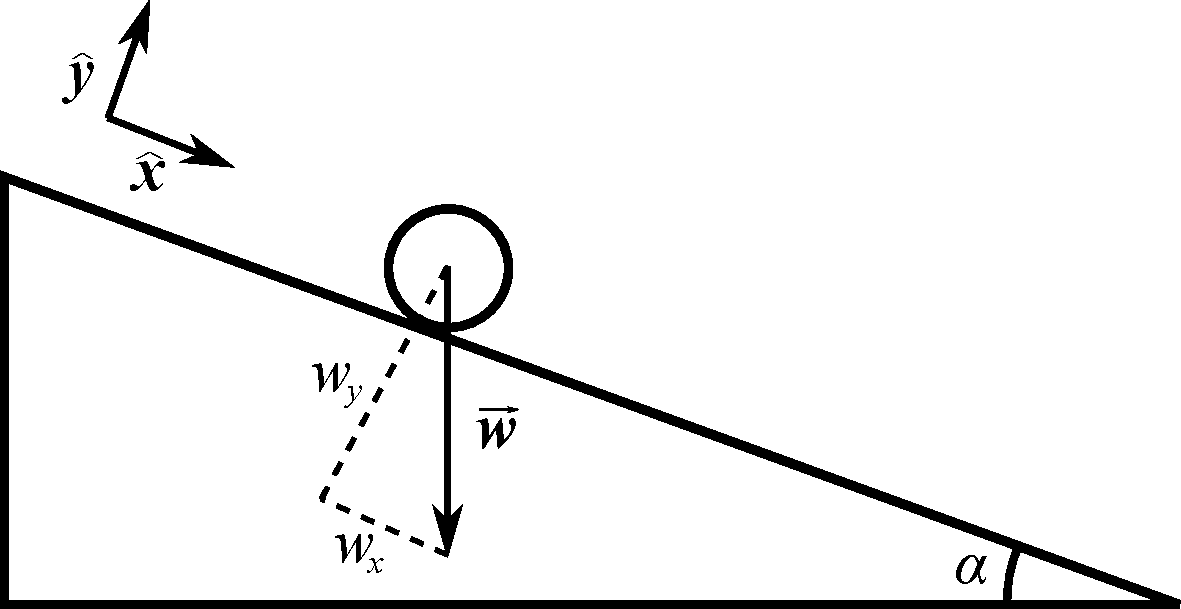
\includegraphics[width=.6\columnwidth]{Analytisk-Mekanik/Cylinder.pdf}
\caption{Eksempel på bevarelse af spørgsmålene 1 og 2 i opgave \ref{opg:cylinder}. Vinklen $\alpha$ skal lokaliseres, $x$ skal defineres parallelt med skråplanet og identificeres som generaliseret koordinat.}
\label{fig:Cylinder}
\end{figure}
%
%
\begin{opgave}{Cylinder på skråplan}{2}
\opg Se figur \ref{fig:Cylinder}.
\opg Fremgår ligeså af figuren.
\opg Den potentielle energi opskrives ud fra højden over bunden af skråplanet $h = x\sin(\alpha)$. Dermed bliver den potentielle energi
\begin{align*}
	V = mg\sin(\alpha)x \: .
\end{align*}
\opg Den kinetiske energi er
\begin{align*}
	K &= \frac{1}{2}m\dt{x}^2 + \frac{1}{2}I\omega^2 \\
	&= \frac{1}{2}m\ddt{x}^2 + \frac{1}{2}I\left(\frac{\dt{x}}{^R}\right)^2 \\
	&= \frac{1}{2}\left(m+\frac{I}{R^2}\right)\dt{x}^2 \: ,
\end{align*}
analogt til spørgsmål 1 i opgave \ref{opg:Yoyo}.
\opg Den potentielle energi er
\begin{align*}
	L &= K + V = \frac{1}{2}\left(m+\frac{I}{R^2}\right)\dt{x}^2 - mg\sin(\alpha)x \: .
\end{align*}
\opg Der differentieres
\begin{align*}
	\pdif{\dt{x}}{L} &= \left(m+\frac{I}{R^2}\right)\dt{x} \: , \\
	\pdif{x}{L} &= -mg\sin(\alpha)x \: , \\
	\implies \el{\dt{x}} &= \left(m+\frac{I}{R^2}\right)\ddt{x} \: .
\end{align*}
Differentialerne løses i rækkefølge som
\begin{align*}
	\pdif{x}{}\frac{1}{2}x^2 &= x \: ,\\
	\pdif{x}{}x &= 1 \: ,\\
	\dif{t}{}\dt{x} &= \ddt{x} \: .
\end{align*}
Nu stoppes ind i Euler-Lagrangeligningen og divideres først med parentesen og til sidst forkortes brøken med $m$:
\begin{align*}
	\el{x} &= \pdif{x}{L} \\
	\implies \ddt{x} &= -\frac{g\sin\alpha}{1+I/mR^2} \: .
\end{align*}
\opg Bevægelsesligningen afhænger ikke $t,x,\dt{x}$, hvorfor der ikke sker nogen ændring i accelerationen mens tiden går.
\opg Bevægelsesligningen skrives på formen
\begin{align*}
	\dif[2]{t}{x} &= \tilde{g} \\
	\implies x &= \int\int\tilde{g}\d t^2 \\ 
	&= \integral{\tilde{g}t + v_0}{t}{}{} \\
	&= \frac{1}{2}\tilde{g}t^2 + v_0t + x_0 : .
\end{align*}
\end{opgave}
%
%
\begin{opgave}{Masse på roterende ring}{3}
Dette problem har mange paralleller til pendulet, hvorfor det kan være relevant at referere til afsnit \ref{k-sec:PendulLagrange} i kompendiet.
\opg Gravitationel potentiel energi er på formen $V=mgh$, og helt ækvivalent til pendulet defineres nulpunktet i $\phi = 0$, hvorved
\begin{align*}
	V(\phi) = mgR\big[1 - \cos(\phi)\big] \: .
\end{align*}
\opg Ligning \eqref{k-eq:SmartFart} i kompendiet siger at $v = r\dt{\phi}$, men den skal lige vendes rigtigt, for at kunne bruges her. Den er udledt for cylinderkoordinater, men gælder generelt for cirkelbevægelser, hvorfor de rigtige cirkler skal identificeres. Hastigheden for lodets bevægelse langs ringen, har radius bliver $R$ og vinkelhastighed $\dt{\phi}$, hvorfor
\begin{align*}
	v_\mathrm{lod} = R\dt{\phi} \: .
\end{align*}
Den anden cirkel kræver lidt mere at forestille sig. Forestiller man sig at massen fastholdes samme sted på ringen, vil den være i jævn cirkelbevægelsen i planet ortogonalt på tegningen. Denne cirkelbevægelse har vinkelhastighed $\omega$ og radius $\rho$, og trigonometri kan bruges til at udtrykke $\rho$ ved $\phi$.
\begin{align*}
	v_\mathrm{ring} = \rho\omega \xleq{\rho = R\sin(\phi)} R\omega\sin(\phi) \: .
\end{align*} 
\opg Den totale kvadrerede hastighed bliver nu summen af kvardraterne på komponenterne
\begin{align*}
	v^2 &= v_\mathrm{lod}^2 + v_\mathrm{ring}^2 \\
	&= R^2\dt{\phi}^2 + R^2\omega^2\sin^2(\phi) \\
	&= R^2\big[\dt{\phi}^2 + \omega^2\sin^2(\phi)\big] \: .
\end{align*}
Ganges dette med $m/2$ fås den kinetiske energi
\begin{align*}
	K = \frac{1}{2}mR^2\big[\dt{\phi}^2 + \omega^2\sin^2(\phi)\big] \: .
\end{align*}
og trækkes den potentielle energi fra fås
\begin{align*}
	L = \frac{1}{2}mR^2\big[\dt{\phi}^2 + \omega^2\sin^2(\phi)\big] - mgR\big[1-\cos(\phi)\big] \: .
\end{align*}
\opg For at benytte Euler-Lagrangeligningen til at bestemme bevægelsesligningen bestemmes følgende differentialer
\begin{align*}
	\pdif{\dt{\phi}}{L} &= mR^2\dt{\phi} \: , \\
	\el{\dt{\phi}} &= mR^2\ddt{\phi} \: , \\
	\pdif{\phi}{L} &= mR^2\omega^2\sin(\phi)\cos(\phi) - mgR\sin(\phi) \: .
\end{align*}
hvor kædereglen skal huskes til differentiation af $\sin^2(\phi)$ i det sidste differential. Euler-Lagrangeligningen siger så at de to sidste differentialer er ens, hvorfor
\begin{equation} \label{eq:BeadOnHoopEOM}
	\begin{aligned}
		\el{\dt{\phi}} &= \pdif{\phi}{L} \\
		mR^2\ddt{\phi} &= mR^2\omega^2\sin(\phi)\cos(\phi) - mgR\sin(\phi) \\
		\ddt{\phi} &= \left[\omega^2\cos(\phi) - \frac{g}{R}\right]\sin(\phi) \: .
\end{aligned}
\end{equation}
\opg Fysisk set er et ligevægtspunkt et sted, hvor et objekt bliver, hvis det placeres der med farten $0$. Stabiliteten kan undersøges ved at placere objektet der med hastigheden nul, og så puffe en smule til det. Accelereres objektet tilbage mod ligevægtspunktet, er ligevægtspunktet stabilt, men accelereres det væk fra er det ustabilt. Som eksempel kan tænkes på en bold i et bakket område. Placeres bolden præcis på toppen af en bakke, så bliver den der, men skubbes der en smule til den, triller den ned af bakken. Derfor er bakketoppen et ustabilt ligevægtspunkt. Placeres bolden dog midt i en bakkedal uden fart, bliver bolden der også, men puffes der til den, vil den rulle lidt op ad bakken inden den ruller ned igen og tilbage til ligevægtspunktet. Derfor er dette punkt stabilt. \\
Kaldes et ligevægtspunkt $\phi_0$, så kan disse kriterier udtrykkes matematisk ved at $\ddt{\phi}|_{\phi=\phi_0} = 0$, hvis $\dt{\phi}|_{\phi=\phi_0} = 0$ og $\phi = \phi_0$. For at undersøge stabiliteten lader man $\phi$ være forskudt både lidt i positiv og i negativ, og hvis $\ddt{\phi}$ så også er har modsat fortegn af forskydningen, er ligevægtspunktet stabilt. Hvis ikke er ligevægtspunktet ustabilt.
\opg Af ovenstående sættes $\ddt{\phi} = 0$
\begin{align*}
	0 = \ddt{\phi} &= \left[\omega^2\cos(\phi) - \frac{g}{R}\right]\sin(\phi) \\
	\implies 0 &= \begin{cases} \omega^2\cos(\phi_0) - \dfrac{g}{R} \vspace{1mm}\\
	\sin(\phi_0) \end{cases} \\
	\implies \phi_0 &= \begin{cases}
	\mathrm{Re}\left[\pm\arccos\left(\dfrac{g}{R\omega^2}\right)\right] \vspace{1mm} \\
	\arcsin(0) = 0,\pm\pi
	\end{cases} \\
	\phi_0 &= \begin{cases}
	\mathrm{Re}\left[\pm\arccos\left(\dfrac{g}{R\omega^2}\right)\right] \vspace{.5mm} \\
	0 \vspace{.5mm} \\
	\pm\pi
	\end{cases}
\end{align*}
Det med at tage realdelen af $\pm\arccos(g/(R\omega^2)$ er en smule pedantisk, men det skyldes at det kun er realdelen, der giver fysisk mening, da fysiske størrelser ikke kan være imaginære. Dette bliver vigtigt senere. Yderligere er både den positive og negative løsning gyldig, hvorfor de begge skal tages med. \vspace{2mm}\\
Det simpleste ligevægtspunkt er $\phi_0 = 0$, hvilket svarer til at massen er i bunden af ringen. \\
$\phi_0 = \pm\pi$ svarer til at massen er i ringens toppunkt. \\
Det sidste ligevægstpunkt er en smule sværere at forestille sig, men det er essentielt set et punkt hvor det at ringen roterer, presser massen opad. Man kan tænke det på samme måde som det at man kan få et pendul til svinge i pæne cirkler.
\opg Der en to eller fire ligevægtspunkter alt efter fortegnet for differencen $\omega^2 - g/r$, fordi det øverstående ligevægtspunkt ikke altid eksisterer. Dette kan forklares ud fra bevægelsesligningen. Kigges på differentialligningen fås dette ligevægtspunkt ved ligningen
\begin{align} \label{eq:phi0_def}
	0 = \omega^2\cos(\phi_0) - \dfrac{g}{R} \: .
\end{align}
Da $\cos(\phi)$ altid giver værdier mellem $-1$ og $1$, ligegyldig hvilket $\phi$, der vælges, kan dette ligevægtspunkt kun eksistere, hvis $\omega^2>g/R$, eftersom ligningen ikke har nogen løsning for $g/R>\omega^2$.
\opg Intuitivt set er $\phi_0=\pm\pi$ ustabil, da tyngdekraften jo vil trække massen ned, hvis den flyttes bare en smule væk fra toppunktet, hvilket gør punktet ustabilt. Matematisk set så bliver $\cos(\phi)$ negativ, hvis $\phi\approx\pm\pi$, hvorfor hele parentesen i ligning \eqref{eq:BeadOnHoopEOM} er negativ. $\sin(\pm\pi)=0$, hvis $\phi<\pi$ er $\sin(\phi)>0$, og omvendt for $\phi<-\pi$. Skubbes massen nu fra $\phi=\pi$ i retningen så $\phi$ bliver mindre, så bliver $\sin(\phi)>0$, men da frontfaktoren er negativ, så vil den accelereres i negativ retning. Helt analogt sker det samme hvis massen var blevet skubbet til den anden side, hvorfor ligevægtspunktet er ustabilt. \\[2mm]
Umiddelbart ville man tro at $\phi_0=0$ og $\phi_0=\mathrm{Re}\big[\pm\arccos(g/(R\omega^2))\big]$ er stabile begge to, men det viser sig at $\phi_0=0$ er ustabil i nogle tilfælde. Dette kan vises ved en Taylorudvikling til første orden omkring $0$. Her bliver bevægelsesligningen
\begin{align*}
	\ddt{\phi} \simeq \left[\omega^2 - \frac{g}{R}\right]\phi = k\phi \: .
\end{align*}
hvor $k$ bare er kort notation for alt det i parentesen. Placeres massen i $\phi = 0$ med hastighed $\dt{\phi}=0$ er $\ddt{\phi}=0$, hvorefter der puffes en smule til massen, så $\phi>0$, får $\ddt{\phi}$ samme fortegn som $k$, hvilket betyder at $\phi_0 = 0$ er stabilt, hvis $k<0$. Dette er tilfældet hvis $\omega^2<g/R$, med andre ord hvis ringen roterer langsomt. Hvis ringen roterer hurtigt, er $k>0$, hvorfor $\phi_0=0$ bliver ustabilt, men til gengæld skaber dette de to nye ligevægtspunkter. \vspace{2mm}\\
Ligevægtspunktet $\phi_0=\mathrm{Re}\big[\pm\arccos(g/(R\omega^2))\big]$ er stabilt, hvilket kan vises ved en lettere træls Taylorudvikling til 1. orden. Dette forventes ikke at deltagerne kan gøre, men for de interesserede, gøres det således. Først omkrives bevægelsesligning således at nulpunktet flyttes til ligevægtspunktet - dvs. $\phi \rightarrow \phi_0 + \epsilon$, hvor $\epsilon$ er en lille forskydning. $\phi_0$ er defineret som en konstant, hvorfor $\ddt{\phi} = \ddt{\epsilon}$, og derved bliver 
\begin{align*}
	\ddt{\epsilon} = \left[\omega^2\cos(\phi_0 + \epsilon) - \frac{g}{R}\right]\sin(\phi_0 + \epsilon) \: .
\end{align*}
Dette Taylorudvikles omkring $\epsilon=0$, hvilket giver
\begin{align} \label{eq:epsilon}
	\ddt{\epsilon} \simeq \left[\omega^2\Big(\cos(\phi_0)-\epsilon\sin(\phi_0)\Big) - \frac{g}{R}\right]\left[\sin(\phi_0) + \epsilon\cos(\phi_0)\right] \: .
\end{align}
Dette skyldes at følgende Taylorudviklinger benyttes
\begin{align*}
	\cos(\phi_0 + \epsilon) &\simeq \cos(\phi_0) - \epsilon\sin(\phi_0) \: , \\
	\sin(\phi_0 + \epsilon) &\simeq \sin(\phi_0) + \epsilon\cos(\phi_0) \: .
\end{align*}
Det virker måske lidt mærkeligt at leddene $\cos(\phi_0)$ og $\sin(\phi_0)$ er med her, men det skyldes at når differentialerne i Taylorrækken evalueres, så fås
$\cos(\phi_0 + 0) = \cos(\phi_0)$ i stedet for $\cos(0) = 1$. \\[2mm]
Tricket er at udvikle til laveste orden, der giver et brugbart resultat, hvilket her er 1. orden. Derfor udvikles sinus og cosinus til 1. orden, og herefter negligeres eventuelle led af højere orden. Nu benyttes definitionen af $\phi_0$, der kan skrives som i ligning \eqref{eq:phi0_def}, til at reducere ligning \eqref{eq:epsilon}.
\begin{align*}
	\ddt{\epsilon} &\simeq \left[\omega^2\Big(\cos(\phi_0) - \epsilon\sin(\phi_0)\Big) - \frac{g}{R}\right]\Big[\sin(\phi_0) + \epsilon\cos(\phi_0)\Big] \\
	&= -\omega^2\epsilon\Big[\sin(\phi_0) + \epsilon\cos(\phi_0)\Big] \\
	&\simeq -\omega^2\sin(\phi_0)\epsilon \: .
\end{align*}
Andenordensledet kastes væk idet der udvikles til 1. orden, og det ses nu at $\epsilon$ opfører sig som en harmonisk oscillator til første orden. Det med at kaste andenordensledet væk er en formel ting, idet man ikke kan vide noget om dette, da man ikke har taget andenordensledene med for sinus og cosinus, hvorfor der kommer til at mangle noget for at have en korrekt udvikling til 2. orden. Havde man udviklet til første orden og fundet ud af at approksimationen ikke giver en nogen brugbar information, så kan man ikke bare tage eventuelle negligerede højereordensled med igen. Det eneste rigtige er så at beslutte sig for en højere orden at approksimere til, og så starte forfra med approksimationen. Man er ofte interesseret i bevægelsen omkring et stabilt ligevægtspunkt, hvorfor denne type beregning er relativt almindelig.
\end{opgave}
%
%
\section*{Flerlegemeproblemer}
%
%
\begin{opgave}{To koblede vogne}{2}
\opg Først opskrives den lille vogns stedkoordinat, der kaldes $r$
\begin{align*}
	r = x + X \: .
\end{align*}
Dette differentieres
\begin{align*}
	\dt{r} = \dt{x} + \dt{X} \: ,
\end{align*}
hvorved
\begin{align*}
	K = \frac{1}{2}m\dt{r}^2 = \frac{1}{2}m(\dt{x} + \dt{X})^2 \: .
\end{align*}
Navngivningen af koordinatet $r$ er arbitrært og har ingen betydning for opgaven.
\opg Den store vogn drives til harmonisk oscillation på en måde vi ikke bekymrer os om. Den eneste kobling fra den lille vogn til omverdenen er igennem fjereden, da den bevæger sig friktionsløst, hvorfor den potentielle energi er den for en fjeder, altså
\begin{align*}
	V = \frac{1}{2}kx^2 \: .
\end{align*}
Da $L = K - V$ er Lagrangefunktionen
\begin{align*}
	L = \frac{1}{2}m\dt{r}^2 - \frac{1}{2}kx^2 = \frac{1}{2}m(\dt{x} + \dt{X})^2 - \frac{1}{2}kx^2 \: .
\end{align*}
\opg Nu differentieres på samme måde som i opgave \ref{opg:cylinder}
\begin{align*}
	\pdif{\dt{x}}{L} &= \frac{1}{2}m(2\dt{x} + 2\dt{X}) = m(\dt{x} + \dt{X}) \: , \\
	\pdif{x}{L} &= -kx \: ,
\end{align*}
hvor det første kan løses enten ved kædereglen, eller ved at bruge 1. kvadratsætning inden der differentieres.
\opg Nu løses differentieres i bund
\begin{align*}
	\el{\dt{x}} &= m(\ddt{x} + \ddt{X}) \; ,
\end{align*}
hvorefter $\ddt{X}$ bestemmes ved at differentiere cosinus to gange med kædereglen
\begin{align*}
	\ddt{X} &= \dif[2]{t}{}A\cos(\omega t) = \dif{t}{}(-A\omega\sin(\omega t)) = -A\omega^2\cos(\omega t) \: .
\end{align*}
Dette stoppes ind i Euler-Lagrangeligningen
\begin{align*}
	\el{x} &= \pdif{x}{L} \\
	\implies m(\ddt{x} - A\omega^2\cos(\omega t)) &= -kx \\
	\implies \ddt{x} + \frac{k}{m}x &= A\omega^2\cos(\omega t) \\\implies \ddt{x} + \omega_0^2x &= A\omega^2\cos(\omega t) \: .
\end{align*}
\opg Indsættes $A=0$ i bevægelsesligningen fås
\begin{align*}
	\ddt{x} + \omega_0x &= 0\cdot\omega^2\cos\omega t = 0 \\
	\ddt{x} &= -\omega_0x \: .
\end{align*}
hvilket er en simpel harmonisk oscillator.
\opg Det er relevant at tjekke denne grænse, da det fungerer som en konsistens kontrol, der er meget almindelig i fysik. Når der er regnet noget kompliceret, så kigges på en grænse, hvori bevægelsesligningen bør reducere til noget kendt. I tilfældet her er det "kendte tilfælde"\;en vogn på en fjeder. \\
\paragraph{Perspektiverende:} I elektromagnetisme bruger man ofte at hvis man er tilpas langt væk fra nogle ladninger, så ligner de bare en punktladning, hvorfor man tjekker grænsen $r\rightarrow\infty$ hvor $r$ er afstanden til et defineret nulpunkt tæt på ladningerne og i denne grænse bare er afstanden til ladningerne.
\end{opgave}
%
%
\begin{figure}[t]
\centering
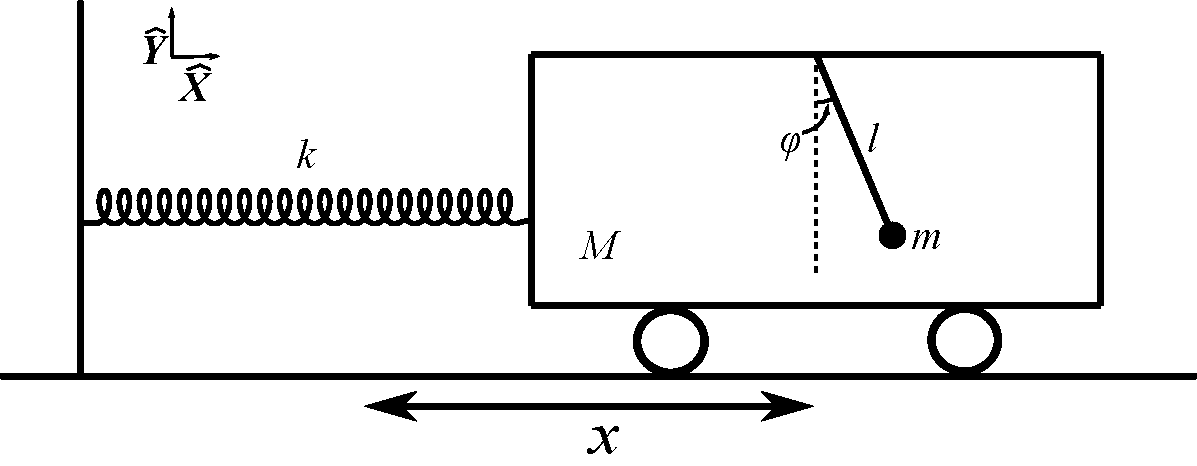
\includegraphics[width=.6\columnwidth]{Analytisk-Mekanik/PendulIVogn.pdf}
\caption{Illustration af situationen med indtegnet kartesisk koordinatsystem og genereliserede koordinater.}
\label{fig:PendulIVogn}
\end{figure}
%
%
\begin{opgave}{Pendul i en vogn}{4}
\opg Origo defineres som ophængningspunktet for pendulet for $X=0$, og koordinatsystemet placeres således at tyngdekraften er i $Y$-retningen og fjederkraften er i $X$-retningen, se figur \ref{fig:PendulIVogn}.
\opg De kartesiske koordinater for pendullodets position er
\begin{align*}
	X_p &= x + l\sin\phi \: , \\
	Y_p &= l\cos\phi \: .
\end{align*}
og for vognet er $Y_v$ uændret, da den kun kan bevæge sig langs $\hat{X}$, hvorfor den er ubetydelig. Slutteligt er
\begin{align*}
	X_v = x \: .
\end{align*}
\opg Vognens forskydning er den eneste, som betyder noget for fjederen, og pendullodets vertikale position bruges til den gravitationelle den, hvorved
\begin{align*}
	V = \frac{1}{2}kx^2 + mgl(1-\cos\phi) \: .
\end{align*}
\opg Differentieres de kartesiske koordinater fås
\begin{align*}
	\dt{X}_p &= \dt{x} + l\dt{\phi}\cos\phi \: , \\
	\dt{Y}_p &= l\dt{\phi}\sin\phi \: , \\
	\dt{X}_v &= \dt{x} \: .
\end{align*}
Det ses at idiotformlen kan anvendes ved kvadrering, analogt til ligning \eqref{k-eq:SmartFart} i kompendiet, hvorved der opnås
\begin{align*}
	K = \frac{1}{2}M\dt{x} + \frac{1}{2}m\big[\dt{x}^2 + l^2\dt{\phi}^2 + 2l\dt{x}\dt{\phi}\cos\phi\big] \: .
\end{align*}
hvorfor Lagrangefunktionen bliver
\begin{align*}
	L = \frac{1}{2}M\dt{x} + \frac{1}{2}m\big[\dt{x}^2 + l^2\dt{\phi}^2 + 2l\dt{x}\dt{\phi}\cos\phi\big] - \frac{1}{2}kx^2 + mgl(1-\cos\phi) \: .
\end{align*}
\opg Differentialerne  for $x$ bestemmes
\begin{align*}
	\pdif{\dt{x}}{L} &= M\dt{x}+ m\dt{x} + ml\dt{\phi}\cos\phi \: , \\
	\pdif{x}{L} &= -kx \: ,\\
	\el{\dt{x}} &= M\ddt{x}+ m\ddt{x} + ml(\ddt{\phi}\cos\phi - \dt{\phi}^2\sin\phi) \: ,
\end{align*}
hvilket giver differentialligningen
\begin{align*}
	a) \qquad M\ddt{x} + m\ddt{x} + ml\ddt{\phi}\cos\phi - ml\dt{\phi}^2\sin\phi &= -kx \: .
\end{align*}
Differentialerne for $\phi$ bestemmes
\begin{align*}
	\pdif{\dt{\phi}}{L} &= ml^2\dt{\phi} + ml\dt{x}\cos\phi \: , \\
	\pdif{\phi}{L} &= -ml\dt{x}\dt{\phi}\sin\phi - mgl\sin\phi \: ,\\
	\el{\dt{\phi}} &= ml^2\ddt{\phi} - ml\dt{x}\dt{\phi}\sin\phi + ml\ddt{x}\cos\phi \: ,
\end{align*}
så differentialligningen bliver
\begin{align*}
	b) \qquad ml^2\ddt{\phi} + ml\ddt{x}\cos\phi &= -mgl\sin\phi \: .
\end{align*}
\opg Til første orden er $\cos\phi \simeq 1$, mens $\sin\phi \simeq \phi$ hvorved 
\begin{align*}
&a) \quad M\ddt{x} + m\ddt{x} +ml\ddt{\phi} \simeq -kx \\
&b) \quad \ddt{\phi} + \frac{\ddt{x}}{l} \simeq -\frac{g}{l}\phi
\end{align*}
\opg Den svarer til følgende scenarier \\
1. \quad $k \rightarrow \infty$ betyder at modstanden i fjederen bliver uendelig stor. \\
2. \quad Vognen er meget tungere end pendulet, som med andre ord betyder at vognen bevæger som om pendulet ikke var der.
\opg I de optalte grænser reducerer systemet til følgende situationer \\
1. \quad Modstanden i fjederen er så stor at vognen bevægelse bliver negligibel, hvorfor det forventes at pendulet opfører sig på sædvanlig vis, det vil sige en harmonisk oscillator\footnote{Den harmoniske oscillator kaldes også engang imellem simpel harmonisk bevægelse, forkortet SHB.}. \\
2. \quad Pendulets masse er så lille at dettes eksistens er ubetydelig for vognen, der så vil opføre sig som en vogn på en fjeder, altså en harmonisk oscillator. Det betyder for pendulet at dets ophængningspunkt vil oscillere harmonisk, hvorfor der forventes en drevet svingning af pendulet.
\opg Kigges på bevægelsesligningerne gøres følgende observationer \\
1. \quad Da $k$ er uendelig stor må $x$ være uendelig lille for at opfylde bevægelsesligningen og ligning $a$ mister herved betydning. Dette skal gælde til alle tider, så derfor må de tidsaflede af $x$ også være meget små, hvorfor de negligeres i $b$. Den eneste bevægelsesligning med betydning bliver derfor
\begin{align*}
	b) \quad \ddt{\phi} &= -\frac{g}{l}\phi = -\omega_1^2\phi \\
\phi &= A_1\cos(\omega_1t + \delta_1)
\end{align*}
hvor $A_1$ og $\delta_1$ begge er konstanter bestemt af startbetingelserne. \\
2. \quad Pendulets masse er negligibel ift. vognen, hvorfor led med $m$ negligeres fra bevægelsesligning $a$.
\begin{align*}
	a) \quad \ddt{x} &= -\frac{k}{M}x = -\omega_2^2x \\
	x &= A_2\cos(\omega_2t + \delta_2)
\end{align*}
hvor $A_2$ og $\delta_2$ igen er konstanter bestemt af startbetingelserne. Indsættes dette i bevægelsesligning $b$ fås
\begin{align*}
b) \quad \ddt{\phi} + \omega_1^2\phi = \frac{A\omega_2^2}{l}\cos(\omega_2t + \delta_2)
\end{align*}
hvor $\delta_2$ også er en konstant. Løsningen til denne differentialligning er træls, men det er en drevet harmonisk svingning. \vspace{2mm}\\
Konkluderende kan det siges at bevægelsesligningerne reducerer pænt til forventelige resultater i nogle udvalgte grænser, hvilket er en god indikator for deres validitet.
\end{opgave}
%
%
\section*{Fiktive Kræfter}
%
%
\begin{opgave}{Fysiske og fiktive kræfter}{2}
\opg Det antages at systemet er stedafhængigt, hvilket vil sige at der udelukkende indgår variable i sted, hvilket eksempelvis kunne være de kartesiske koordinater $(x,y)$, og konstanter i den potentielle energi. $V(x,y)$ er dermed konstant overfor hastigheder $(\dt{x},\dt{y})$, hvorfor de partielt afledede mht. disse er $0$.
\opg Af spørgsmål 1 er det led den potentielle energi bidrager til ledet $\el{\dt{q}_i}$ med $0$, hvis tidsafledede også er nul. Dermed er $\dif{t}{}\left(\pdif{\dt{q}_i}{V}\right)=0$, hvilket giver den efterspurgte konklusion.
\opg Eftersom den potentielle energi kun bidrager med et additivt led til delen af Euler \hspace{-0.1cm}- \hspace{-0.1cm}Lagrangeligningen, der er den generaliserede kraft, tilføjes differentialerne med negativt fortegn på den side af lighedstegnet, grundet  på Lagrangefunktionen.
\opg Venstre side af lighedstegnene er masse gange acceleration, og summen af fysiske kræfter kan udtrykkes som den negative gradient af den samlede potentielle energi. Det betyder at hvis de fiktive kræfter betragtes som kræfter, så er ligningerne fra Newtons 2. lov i to forskellige dimensioner. Defineres de fiktive kræfter som i eksemplet opfører de sig dermed overfor Newtons 2. lov som enhver anden fysisk kraft.
\end{opgave}
%
%
\begin{figure*}
	\centering
	\includegraphics[width=.9\textwidth]{Analytisk-Mekanik/ToMasserRoterendeStangFiktivekrafter.pdf}
	\caption{De fiktive kræfter er her indtegnet hvor $m$, $\Omega$ og $\dt{\rho}_1$ er antaget positive.} \label{fig:ToMasserRoterendeStangFiktivekraefter}
\end{figure*}
%
%
\begin{opgave}{To masser på en roterende stang}{3}
\opg Systemet roterer i et plan omkring et fast punkt, hvorfor cylindrisk polære koordinater er oplagt.
\opg Da stangen er antaget stiv, kan loddernes bevægelse i $\phi$-retningen kun komme fra stangens rotation, som er antaget konstant. Da $\rho_1$ og $\rho_2$ er koblede er det generaliserede koordinat derfor enten $\rho_1$ eller $\rho_2$, og her vælges $\rho_1$.
\opg Da stangens længde er konstant er
\begin{align*}
	0 = \dif{t}{l}& = \dt{\rho}_1 + \dt{\rho}_2 \\
	\dt{\rho}_1 &= -\dt{\rho}_2
\end{align*}
\opg Ligning \eqref{k-eq:FiktiveKraefter} i kompendiet siger at\footnote{cor/cf står som superscript og ikke subscript for at gøre det mere overskueligt. Der er ikke anden grund.}
\begin{align*}
	\v{F}^\mathrm{cor} &= 2m\dt{\v{r}}\times\v{\Omega} \: , \\
	\v{F}^\mathrm{cf} &= m(\v{\Omega} \times \v{r}) \times \v{\Omega} \: .
\end{align*}
hvor de generaliserede koordinater på vektorform er
\begin{align*}
	\v{\rho}_1 &= \rho_1\rhat \: , \\
	\v{\rho}_2 &= \rho_2\rhat = (l-\rho_1)\rhat \: ,\\
	\dt{\v{\rho}}_1 &= \dt{\rho}_1\rhat \: , \\
	\dt{\v{\rho}}_2 &= \dt{\rho}_2\rhat = -\dt{\rho}_1\rhat \: .
\end{align*}
Stangen roterer omkring $z$-aksen, hvorfor $\v{\Omega} = \Omega\zhat$. Derfor bliver de fiktive kræfter
\begin{align*}
	\v{F}_1^\mathrm{cor} &= 2m_1\dt{\rho}_1\Omega\rhat\times \zhat \\
	&= -2m_1\dt{\rho}_1\Omega\phhat \: , \\
	\v{F}_1^\mathrm{cf}	&= m_1\rho_1\Omega^2(\zhat \times \rhat) \times \zhat \\
	&= m_1\rho_1\Omega^2(\phhat \times \zhat) \\
	&= m_1\rho_1\Omega^2\rhat \: , \\
	\v{F}_2^\mathrm{cor} &= 2m_2(-\dt{\rho}_2)\Omega\rhat\times \zhat \\
	&= 2m_2\dt{\rho}_2\Omega\phhat \\
	&= -2m_2\dt{\rho}_1\Omega\phhat \: , \\
	\v{F}_2^\mathrm{cf} &= m_2\rho_2\Omega^2(\zhat \times \rhat) \times \zhat \\
	&= m_2\rho_2\Omega^2(\phhat \times \zhat) \\
	&= m_2\rho_2\Omega^2\rhat \\
	&= m_2(l-\rho_1)\Omega^2\rhat \: .
\end{align*}
\opg Antages $m$, $\Omega$ og $\dt{\rho}_1$ for at være positive fås figur \ref{fig:ToMasserRoterendeStangFiktivekraefter}.
\opg Corioliskraften virker på begge legemer i $\phhat$-retningen, men stangen er antaget stiv, hvorfor den påvirker legemerne med en ligestor og modsatrettet normalkraft, hvilket er samme argument som for at $\phi$ ikke er et generaliseret koordinat.
\opg I systemets ligevægtskonfiguration er de to centrifugalkræfters vektorsum nul
\begin{align*}
	\v{F}_1^\mathrm{cf} + \v{F}_2^\mathrm{cf} &= \v{0} \\
	\implies m_1\rho_1\Omega^2 &= m_2\rho_2\Omega^2 \\
	\implies \frac{m_1}{m_2} &= \frac{\rho_2}{\rho_1} = \frac{l}{\rho_1} - 1 \: .
\end{align*}
Vektoren $\rhat$ peger i hver sin retning for de to masser, hvorfor fortegnene passer. Af tegningen fremgår det at de er modsatrettet, og deres størrelser skal så være ens, hvilket er benyttet her.
\opg Hvis masserne er ens forventes legemerne at placere sig lige langt fra rotationspunktet, dvs. $\rho_1 = \rho_2$.
\opg Indsættes de forventede omstændigheder fås
\begin{align*}
	\frac{m_1}{m_1} = \frac{\rho_1}{\rho_1} \quad \checkmark
\end{align*}
\end{opgave}
%
%
\begin{opgave}{Er fiktive kræfter trælse?}{3}
\opg Corioliskraften afhænger af hastighed, mens centrifugalskaften afhænger af position.
\opg Typisk er kræfter stedafhængige, hvilket gælder f.eks. gravitation, fjederkræfter og elektriske kræfter. Derfor giver centrifugalkraften "bare"\;en ekstra stedafhængighed, hvilket ikke er helt umuligt, mens hastighedsafhængigheden af Corioliskraften gør den bøvlet at arbejde med.
\opg Denne differentialligning minder ret så meget om
\begin{align*}
	\dif{t}{g(t)} = kg(t)
\end{align*}
Den minder faktisk så meget om, at de er ens hvis $g(t) = \dif{t}{f(t)}$
\begin{align*}
	\dif{t}{}\left(\dif{t}{f(t)}\right) = k\left(\dif{t}{f(t)}\right) \: ,
\end{align*}
hvorfor løsningen af denne differentialligningen kan bruges
\begin{align*}
	\dif{t}{f(t)} = g(t) = A\exp(kt) \: ,
\end{align*}
hvor separation af de variable kan benyttes
\begin{align*}
	\d f &= A\exp(kt)\d t \\
	\int \d f &= \int A\exp(kt)\d t \\
	f(t) &= \frac{A}{k}\exp(kt) + B \: .
\end{align*}
Her er konstanterne fra begge ubestemte integraler lagt ind i konstanten $B$.
\end{opgave}
%
%
\section*{Perspektiverende Problemer}
%
%
\begin{opgave}{Tennis Racket Theorem}{4}
Det vigtige her er først at forstå antagelsen om de små vinkelaccelerationer. Eksempelvis er $\omega_y$ ikke lille nok til at se bort fra alle led, der indeholder $\omega_y$, men den er lille nok til at $\omega_y^2 \approx 0$, hvorfor alle led der indeholder $\omega_y^2$, $\omega_z^2$ eller $\omega_y\omega_z$ kan negligeres.
\opg Derved er
\begin{align*}
	\dif{t}{}\left(I_x\dt{\omega}_x\right) \simeq \dif{t}{}\left[(I_y-I_z)(0)\right] = 0 \: .
\end{align*}
Generelt set er
\begin{align*}
	\dif{t}{}(\omega_i\omega_j) = \dt{\omega}_i\omega_j + \omega_i\dt{\omega}_j \: .
\end{align*}
Vi har dog lige argumenteret for at $\dt{\omega}_x \simeq 0$, hvilket betyder led, der afhænger af $\dt{\omega}_x$ negligeres. Herved opnås ligning \eqref{eq:TRT_DiffLignX} ved at differentiere den anden vinkelhastighed.
\opg I ligning \eqref{eq:TRT_DiffLign} isoleres de relevante førsteafledede og så indsættes det i ligning \eqref{eq:TRT_DiffLignX}.
\opg Eftersom $I_x>I_y$ er $I_x-I_y > 0$, mens $I_z<I_x$, hvorfor $I_z-I_x<0$. Vinkelhastighederne er reelle, hvorfor
\begin{align*}
	\omega_x^2(I_z-I_x)(I_x-I_y) < 0 \: .
\end{align*}
Idet inertimomenterne er positive størrelser, ændres fortegnet ikke at at dividere med $I_y$ eller $I_z$, hvilket betyder at $\ddt{\omega}_i \propto -\omega_i$ for $i=y,z$, hvilket er den ønskede konklusion.
\opg I første omgang differentieres, hvor det huskes at andenordensled i $\omega_x$ og $\omega_z$ negligeres
\begin{align*}
	\dif{t}{}\xyz{I_x\dt{\omega}_x}{I_y\dt{\omega}_y}{I_z\dt{\omega}_z} = \xyz{(I_y-I_z)\omega_y\dt{\omega}_z}{0}{(I_x-I_y)\dt{\omega}_x\omega_y} \: .
\end{align*}
Bruges ligning \eqref{eq:TRT_DiffLign} her til at substituere i de enkeltafledede fås ligning \eqref{eq:TRT_DiffLignY}.
\opg Analogt til spørgsmål 3) fås at $(I_y-I_z)$ og $(I_x-I_y)$ er positive, hvorfor
\begin{align*}
	\omega_y^2(I_x-I_y)(I_y-I_z) > 0 \: ,
\end{align*}
hvor fortegnet igen ikke ændres af at dividere med $I_x$ eller $I_z$.
\opg Hvis rotationen skal være stabil, så må legemet ikke bevæge sig ret meget omkring de andre akser. Har $\ddt{\omega}_j$ samme fortegn som $\omega_j$ så vil vinkelhastigheden øges eksponentielt i tiden, hvorfor legemets rotation om den $j$'te akse øges kraftigt, hvis den ikke starter med en startvinkelhastighed $\omega_j = 0$. Dette betyder at legemets rotation vil starte en rotation om de sekundære\footnote{Den primære rotationsakse er den akse med ikke-lille startværdi af vinkelhastigheden, mens de sekundære akser er dem, hvor startrotationen er lille.} akser, hvorfor rotationen er ustabil. Har $\omega_j$ og $\ddt{\omega}_j$ modsat fortegn så vil vinkelhastighed oscillere omkring 0. Det betyder at legemets rotation får vinklen ved de sekundære akser til at holde sig omkring deres startværdi grunden antagelsen om små vinkelhastigheder.
\opg Fra spørgsmål 3) og spørgsmål 5) samt opgaveteksten til spørgsmål 7 har vi at rotationen om de sekundære akser accelereres, hvis $y$-aksen er den primære rotationsakse, mens der induceres en oscillation omkring de sekundære akser, hvis $x$ eller $z$ er den primære akser. Derved er $y$-aksen ustabil, mens de andre to er stabile.
\opg For en kasse, bog eller andet rektangulært objekt er det således
%
%
\begin{figure}[!h]
\centering
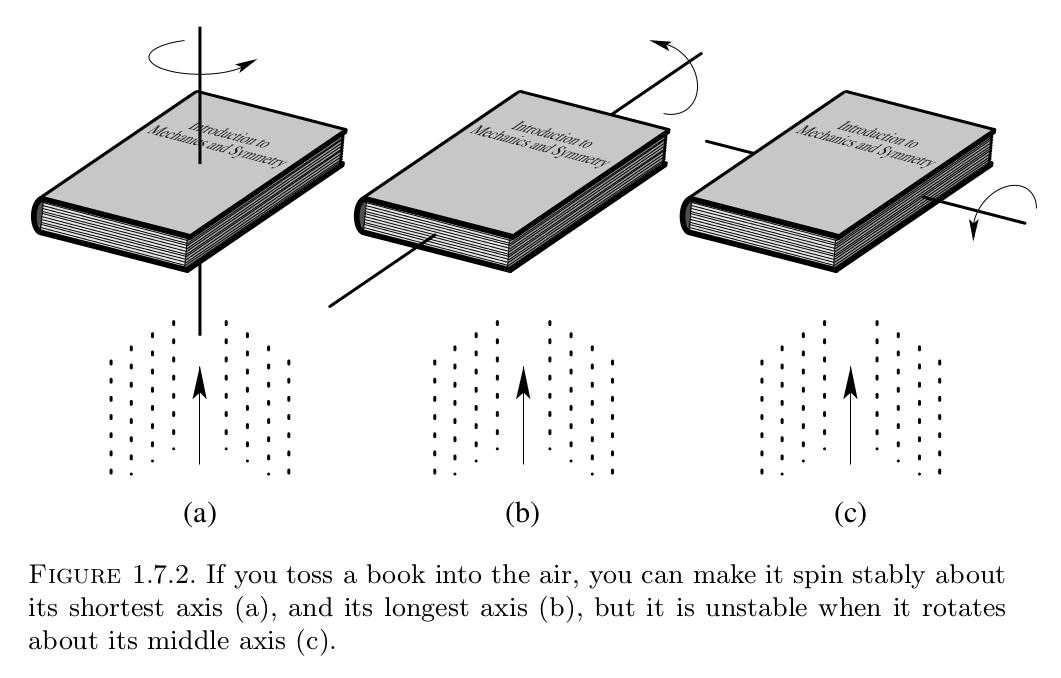
\includegraphics[width=.85\columnwidth]{Analytisk-Mekanik/Rotationsakser.png}
\caption{Illustration af en bog, der roterer med forskellige primærakser, samt en beskrivelse af deres stabilitet.}
%\caption{Kilde: \newline \url{https://physics.stackexchange.com/questions/67957/stability-of-rotation-of-a-rectangular-prism0}}
\end{figure}
\end{opgave}
%
%
\begin{opgave}{Hamiltonfunktionen og et systems energi}{3}
\opg $L = \frac{1}{2}A(q)\dt{q}^2 - V(q)$.
\opg $p = \pdif{\dt{q}}{L} = A(q)\dt{q}$.
\opg $\dt{q} = \frac{p}{A(q)}$.
\opg $H = p\dt{q} - L = \frac{p^2}{A(q)} - \left( \frac{p^2}{2A(q)} - V(q)\right) = \frac{p^2}{2A(q)} + V(q)$.
\opg Der er to måder at vise dette på. Den mest stringente er at starte med energien, udtrykt ved sted og impuls er
\begin{align*}
	E = K + V = \frac{1}{2}A(q)\dt{q}^2 + V(q) = \frac{p^2}{2A(q)} + V(q) = H \: .
\end{align*}
Den anden metode er følgende: Pr. antagelse er $K = \frac{1}{2}A(q)\dt{q}^2$. Dette omskrives nu ved den generaliserede impuls fra spørgsmål 3)
\begin{align*}
	K &= \frac{1}{2}A(q)\dt{q}^2 \\
	&= \frac{1}{2}A(q)\left(\frac{p}{A(q)}\right)^2 \\
	&= \frac{p^2}{2A(q)} \: .
\end{align*}
Indsættes det i Hamiltonfunktionen fra spørgsmål 4) fås definitionen på total energi
\begin{align*}
	H &= \frac{p^2}{2A(q)} + V(q) = K + V = E \: .
\end{align*}
\opg Taleargumentet lyder på at ingen af disse argumenter bygger på andet end antagelsen om formen af energierne. Derfor ændres intet når der tilføjes flere koordinater og der summeres. \\
Et mere matematisk argument er at den kinetiske energi nu skrives på formen
\begin{align*}
	K = \sum_i\frac{1}{2}A(q_i)\dt{q}_i^2 \: ,
\end{align*}
mens den potentielle energi er $V(q_1,q_2,...,q_n)$. Derfor er Lagrangefunktionen
\begin{align*}
	L = \sum_i\frac{1}{2}A(q_i)\dt{q}_i^2 -  V(q_1,q_2,...,q_n) \: .
\end{align*}
Benyttes definitionen af generaliseret impuls, samt det faktum at der ingen krydsled er i den del af Lagrangefunktionen, der afhænger af $\dt{q
}_i$, fås at
\begin{align*}
	q_i = \frac{p_i}{A(q_i)} \: .
\end{align*}
Den kinetiske energi kan nu skrives på formen
\begin{align*}
	K = \sum_i\frac{p_i^2}{2A(q_i)} \: ,
\end{align*}
og sættes disse to ligninger ind i definitionen på Hamiltonfunktionen fås
\begin{align*}
	H &= \sum_ip_iq_i - L \\
	&= \sum_ip_i\frac{p_i}{A(q_i)} - \left(\sum_i\frac{p_i^2}{2A(q_i)} -  V(q_1,q_2,...,q_n)\right) \\
	&= \frac{p_i^2}{2A(q_i)} +  V(q_1,q_2,...,q_n) \\
	&= K + V = E \: .
\end{align*}
Som bonusinformation kan det siges, at selvom Hamiltonfunktionen har den omtalte form, så er det ikke nødvendigvis den mest logiske måde at definere systemets energi på. I nogle tilfælde giver det mere mening at definere energien anderledes, hvilket er muligt, da det absolutte energi ikke har den store betydning i sig selv, da det er ændringer i energien, som har betydning for systemets opførsel. Dette benyttes eksempelvis i afsnit \ref{k-sec:PendulLagrange} i kompendiet om beskrivelsen af pendulet i Lagrangeformalismen, hvor den potentielle energi defineres til at være $0$ i pendulets ligevægtspunkt.
\end{opgave}
%
%
\begin{opgave}{Fra klassisk mekanik til kvantemekanik}{3}
Kvantemekanikken bygger på Hamiltonformalismen, hvorfor idéen med denne opgave er at introducere Hamiltonfunktionen, der omskrives til Hamiltonoperatoren, $\op{H}$, som kan betragtes som grundstenen for kvantemekanikken, fordi den tidsuafhængige eller stationære Schrödingerligning kan skrives som egenværdiproblemet
\begin{align}
	\op{H}\psi = E\psi \: .
\end{align}
Her går $\psi$'erne ikke ud med hinanden, da dette er formuleret ved hjælp af den gren af matematikken, der hedder lineær algebra, hvilket gør matematikken meget lettere, når først man har styr på denne matematik\footnote{Der er lidt fyldtekst fra tid til anden idet dette oprindelig var skrevet som en del af kompendiet, og det bliver beholdt, da det ikke er dårlig indformation, selvom det dog ikke er nødvendigt for at løse opgave.}. Hamiltonoperatoren kan opskrives ud fra den klassiske Hamiltonfunktion.
\opg Den generaliserede impuls kan skrives på formen $p = m\dt{q}$, hvorfor $\dt{q} = p/m$. Derved bliver den kinetiske energi
\begin{align} \label{eq:K(p)}
	K = \frac{1}{2}m\dt{q}^2 = \frac{1}{2}m\left(\frac{p}{m}\right)^2 = \frac{p^2}{2m} \: .
\end{align}
\opg Derved giver ligning \eqref{k-eq:H=E} i kompendiet at
\begin{align}
	H = K + V = \frac{p^2}{2m} + V \: .
\end{align}
\opg Sted og impuls skal omskrives til operatorer, mens masse er en partikelegenskab, og ikke en observabel, med tilhørende operator.
\opg Benyttes impulsoperatoren fra tabel \ref{k-tab:operatorer_i_kvant} i kompendiet nu, samt definitionen på tallet $i$, nemlig at $i^2 = -1$ fås Hamiltonoperatoren fra samme tabel
\begin{align}
	\op{x} &= x \Rightarrow \op{V} = V \\
	\op{p}^2 &= \left(-i\hbar\pdif{x}{}\right)^2 = -\hbar^2\pdif[2]{x}{} \\
	\Rightarrow \op{H} &= \frac{\op{p}^2}{2m} + \op{V} = -\frac{\hbar^2}{2m}\pdif[2]{x}{} + V
\end{align}
Der er hermed dannet en bro mellem klassisk mekanik og kvantemekanik, og målet med dette er at vise at en sådan bro eksisterer fremfor en rigid gennemgang af Hamiltonformalismen og dens klassiske mangfoldigheder. \\

Konkluderende kan det siges at metoden til at analysere et kvantemekanisk system er at opskrive systemets kinetiske\footnote{Der er stort set aldrig krydsled i den kinetiske energi, hvorfor dette ofte er trivielt.} og potentielle energi, for derefter at opstille systemets Hamiltonfunktion. Denne omskrives til en Hamiltonoperator, som giver mening for systemet, og derefter løses den staionære Schrödingerligning. Dette kan lyde relativt simpelt, men der kan komme en del komplikationer i forbindelse med eksempelvis skridtet med at omskrive Hamiltonfunktionen til en passende Hamiltonoperator.
\end{opgave}
%
%
\begin{opgave}{Energibevarelse i Hamilton}{4}
\opg Ved partiel differentiation, f.eks. $\partial/\partial t$, betragtes alt andet end den variabel der differentieres med hensyn til som konstanter og der tages dermed ikke højde for at nogle variable kan afhænge af den variabel, der differentieres med hensyn til. Den fuldstændige tidsaflede tager højde for eventuelle implicitte afhængigheder og kædereglen benyttes til at udtrykke disse. Som eksempel kan bruges et generaliseret koordinat $q$
\begin{align*}
	\pdif{t}{q} &= 0 \: , \\
	\dif{t}{q} &= \dt{q} \: ,
\end{align*}
og det illustreres endnu tydeligere ved $q^2$
\begin{align*}
	\pdif{t}{q^2} &= 0 \: ,\\
	\dif{t}{q^2} &= \pdif{q}{q^2}\dif{t}{q} = (2q)\dt{q} = 2q\dt{q} \: .
\end{align*}
\opg Kædereglen benyttes til at skrive den fuldstændigt tidsafledede af en generel Hamiltonfunktion
\begin{align} \label{eq:dHdt}
	\dif{t}{}H(q,p,t) = \pdif{q}{H}\dif{t}{q} + \pdif{p}{H}\dif{t}{p} + \pdif{t}{H} \: .
\end{align}
Dette gøres da en generel éndimensionel Hamiltonfunktion afhænger eksplicit af tid, det generaliserede koordinat og den dertilhørende generaliserede impuls, og med den fuldstændige tidsafledede skal der tages højde for at de to sidstnævnte kan være tidsafhængige.
\opg Hamiltonsligninger siger
\begin{align*}
	\pdif{q}{H} &=  -\dt{p} \: , \\
	\pdif{p}{H} &=  \dt{q} \: .
\end{align*}
Indsættes det i ligning \eqref{eq:dHdt} fås
\begin{align*}
	\dif{t}{H} &= -\dt{p}\dif{t}{q} + \dt{q}\dif{t}{p} + \pdif{t}{H} \: , \\
	\dif{t}{H} &= -\dt{p}\dt{q} + \dt{q}\dt{p} + \pdif{t}{H} \: .
\end{align*}
\opg Dette følger trivielt fra ovenstående spørgsmål
\begin{align*}
	\dif{t}{H} = \pdif{t}{H} \: .
\end{align*}
\opg Hamiltonfunktionen er bevaret i tid, hvis den ikke ændrer sig i tid, hvilket skrives matematisk som $\d H/\d t = 0$, og det er opfyldt hvis $H$ ikke er eksplicit tidsafhængig, altså $\partial H/\partial t = 0$. Da Lagrangefunktionen og Hamiltonfunktionen har samme eksplicitte tidsafhæninghed medfører dette at Hamiltonfunktionen også er bevaret i tid, hvis $\partial L/\partial t = 0$. Dermed er systemets energi bevaret, hvis systemet opfylder at Hamiltonfunktionen er systemets energi og at denne ikke er eksplicit tidsafhængig.
\opg Dette gøres ved at tilføje $i$'er på $q$ og $p$ og summe over disse led
\begin{align*}
	\dif{t}{H} = \sum_i\left[\pdif{q_i}{H}\dif{t}{q_i} + \pdif{p_i}{H}\dif{t}{p_i}\right] + \pdif{t}{H} \: .
\end{align*}
Præcis samme fremgangsmåde benyttes da ingen af argumenterne er specifikke på en sådan måde så de ikke gælder for et arbitrært koordinat.
\begin{align*}
	\dif{t}{H} &= \sum_i\bigg[-\dt{p}\dt{q} + \dt{q}\dt{p}\bigg] + \pdif{t}{H} = \pdif{t}{H} \: ,
\end{align*}
da indholdet af parentesen er nul for alle $i$
\begin{align*}
	-\dt{p}\dt{q} + \dt{q}\dt{p} = 0 \enspace \forall \; i \: .
\end{align*}
Konklusionen er derfor den samme: Hvis Hamilton-/Lagrangefunktionen ikke er eksplicit tidsafhængig, så er systemets energi bevaret.
\end{opgave}
\chapter{Kvantemekanik}
\section*{Uendeligt dyb brønd}
\begin{opgave}{Parabelformet bølgefunktion}{1}\label{kvant:opg:parabel}
Vi ser her på en partikel i en uendelig brønd i intervallet fra $0$ til $L$. Lad bølgefunktionen være:
$$
\psi = Nx(L-x) 
$$
\opg Find $N$ så bølgefunktionen er normeret.
\opg Hvad er forventningsværdien for positionen $\expect x$?
\opg Find forventningsværdien for energien $\expect E$ og sammenlign den fundne energi med grundtilstandsenergien: $\frac{\pi^2\hbar^2}{2mL^2}$.
\opg Er $\psi$ en stationær tilstand?
\end{opgave}
%
\begin{opgave}{Sammensatte bølgefunktioner}{1}
Find normeringskonstanten $N$ og energien $E$ for de følgende bølgefunktioner, der er sammensat af stationære tilstande for den uendelige brønd.
\opg $N(\psi_1+\psi_2)$.
\opg $N(\psi_1-\psi_3)$.
\opg $N(\psi_1+\psi_2-2\psi_3)$.\\
Hint: Udnyt at bølgefunktionerne er ortonormale.
\end{opgave}
%
\begin{opgave}{Den tidsafhængige bølgefunktion}{2}
I en uendelig brønd er bølgefunktionen til tiden $t=0$:
$$
\Psi(x,0) = \frac{1}{\sqrt{5}}(2\psi_1+\psi_2) 
$$
\opg Hvad er $\Psi(x,t)$? Du kan med fordel bruge 
$$
\omega = \frac{E_1}{\hbar} = \frac{\pi^2\hbar}{2mL^2} \, .
$$
\opg Hvad er $\Psi^*(x,t)$?
\opg Skriv $\Psi^*x\Psi$ så simpelt som muligt.
\opg Hvad er $\expect{x(t)}$? \\
Hint:
\begin{align*}
e^{i\theta}+e^{-i\theta} &= 2\cos \theta \, , \\ \matrixel{\psi_n}{x}{\psi_n} &= \frac{L}{2} \, , \\  \matrixel{\psi_1}{x}{\psi_2} &= \frac{-16L}{9\pi^2} \, .
\end{align*}
\end{opgave}
%
\begin{opgave}{En partikel i et kvadrat}{3}
I to dimensioner er den tidsuafhængige Schrödingerligning i kartesiske koordinater:
$$
E\psi(x,y) = \frac{-\hbar^2}{2m}\left(\pdif[2]{x}\psi +\pdif[2]{y}\psi\right) + V(x,y)
$$
Vi vil se på en kvadratisk brønd, i to dimensioner, med sidelængder på $L$. Her er potentialet nul, når $0\leq x\leq L$ og $0\leq y\leq L$.
Antag nu at man kan skrive bølgefunktionen som:
 $$\psi(x,y) = X(x)Y(y) = XY$$
\opg Indsæt $\psi = XY$ i Schrödingerligningen med $V=0$ og isoler $E$.
\opg Energien vil bestå af en bidrag fra $X$ og $Y$, så $E=E_x+E_y$. Opstil differentialligninger i stil med ligning \eqref{k-kvant:eq:infb} i kompendiet for $X$ og $Y$.
\opg Find generelle løsninger til differentialligningerne, bølgefunktionen og de tilhørende energier. Bemærk at der vil være et kvantetal for hver af differentialligningerne. 
\opg Hvad er de fem laveste energier? Skitser bølgefunktionerne med disse energier.
\end{opgave}
%
\begin{opgave}{En partikel i en boks}{3}
I tre dimensioner er den tidsuafhængige Schrödingerligning i kartesiske koordinater:
$$
E\psi(x,y,z) = \frac{-\hbar^2}{2m}\left(\pdif[2]{x}\psi +\pdif[2]{y}\psi+\pdif[2]{z}\psi\right) + V(x,y,z)
$$
Vi vil se på en kubisk boks med en sidelængde på $L$, hvor potentialet er nul, når $x$, $y$ og $z$ alle er imellem 0 og $L$.
Antag at man kan skrive bølgefunktionen som:
$$
\psi(x,y,z) = X(x)Y(y)Z(z) = XYZ
$$
\opg Indsæt $\psi = XYZ$ i Schrödingerligningen med $V=0$ og isoler $E$.
\opg Energien vil bestå af et bidrag fra $X$, $Y$ og $Z$, så $E=E_x+E_y+E_z$. Opstil differentialligninger i stil med ligning \eqref{k-kvant:eq:infb} i kompendiet for $X$, $Y$ og $Z$.
\opg Find generelle løsninger til differentialligningerne, bølgefunktionen og de tilhørende energier. Bemærk at der vil være et kvantetal for hver af differentialligningerne. 
\opg Find de laveste 5 mulige energier udtrykt i $E_1 = \frac{\pi^2\hbar^2}{2mL^2}$ energien for en  endimensionel uendelig brønd med samme brede som boksens sidelængde.
\end{opgave}
\begin{opgave}{Parabelformet bølgefunktion igen}{1}
Denne opgave bygger videre på opgave \ref{kvant:opg:parabel}, så det er en fordel at have lavet denne opgave først. Vi ser igen på en parabelformet bølgefunktion i en uendelig brønd:
$$
\psi=Nx(L-x)
$$
\opg Hvad er $\sigma_x^2 = \expect{x^2}-\expect{x}^2$?

Vi kender allerede $\expect{x}$ og $\abs N^2$ fra opgave \ref{kvant:opg:parabel}.
\begin{align*}
\expect{x} &= \frac{L}{2}\\
\abs N^2 &= \frac{30}{L^5}
\end{align*}
For at finde $\expect{x^2}$ bruges sandwichen:
\begin{align*}
    \expect{x^2}&= \abs N^2 \integral{x^3(L-x)}{x}{0}{L}\\
    &= \frac{30}{L^5}\integral{x^5-2x^4L+x^3L^2}{x}{0}{L}\\
    &= \frac{30}{L^5}\left[\frac{x^6}{6}-\frac{2x^5L}{5}+\frac{x^6}{6}\right]_0^L\\
    &= 30 L^2\left(\frac{15}{60}-\frac{24}{60}+\frac{10}{60}\right)\\
    &= \frac{L^2}{2}
\end{align*}
Nu er usikkerheden:
$$
\sigma_x^2 = \expect{x^2}-\expect{x}^2 = \frac{L^2}{2}-\frac{L^2}{4}=\frac{L^2}{2}
$$
og
$$
\sigma_x = \frac{L}{\sqrt{2}}
$$
\opg Hvad er $\sigma_p^2 = \expect{p^2}-\expect{p}^2$?
Her skal vi bruge at $\op p = -i\hbar\pdif{x}{}$. Så bliver sandwichen:
\begin{align*}
    \expect{p} &= -i\hbar\abs N^2\integral{x(L-x)\pdif{x}{}\left(x(L-x)\right)}{x}{0}{L}\\
    &= \frac{-30i\hbar }{L^5}\integral{x(L-x)(L-2x)}{x}{0}{L}\\
    &= \frac{-30i\hbar }{L^5}\integral{xL^2-3x^2L+2x^3}{x}{0}{L}\\
    &= \frac{-30i\hbar }{L^5}\left[\frac{x^2L^2}{2}-x^3L+\frac{x^4}{2}\right]_0^L\\
    &= \frac{-30i\hbar }{L} \left(\frac{1}{2}-1+\frac{1}{2}\right)\\
    &=0
\end{align*}
Tilsvarende for $\expect{p^2}$, hvor $op p^2 = -\hbar^2\pdif[2]{x}{}$.
\begin{align*}
    \expect{p^2} &= \abs N^2 \integral{x(L-x)\pdif[2]{x}{}\left(x(L-x)\right)}{x}{0}{L}\\
    &= \frac{-30\hbar^2 }{L^5}\integral{x(L-x)(-2)}{x}{0}{L}\\
    &= \frac{60\hbar^2}{L^5}\integral{xL-x^2}{x}{0}{L}\\
    &= \frac{60\hbar^2}{L^5}\left[\frac{x^2L}{2}-\frac{x^3}{3}\right]_0^L\\
    &= \frac{60\hbar^2}{L^5}\left(\frac{L^3}{2}-\frac{L^3}{3}\right)\\
    &= \frac{60\hbar^2}{L^2}\left(\frac{3}{6}-\frac{2}{6}\right)\\
    &= \frac{10\hbar^2}{L^2}
\end{align*}
Så usikkerheden er:
$$
\sigma_p^2 = \expect{p^2} = \frac{10\hbar^2}{L^2}
$$
og:
$$
\sigma_p = \frac{\hbar\sqrt{10}}{L}
$$
\opg Passer det med Heisenbergs usikkerhedsprincip?

Sættes $\sigma_x$ og $\sigma_p$ ind i Heisenbers usikkerhedsprincip findes:
$$
\sigma_x\sigma_p = \frac{L}{\sqrt{2}}\frac{\hbar\sqrt{10}}{L}= \hbar\sqrt{5}\geq\frac{\hbar}{2}
$$
Heisenberg er tilfreds $\ddot \smile$
\end{opgave}

\begin{opgave}{Den frie partikel}{2}
En fri partikel er en partikel der ikke påvirkes af noget potentiale, så $V(x)=0$ for alle $x$
\opg Hvad er $\op H$?

Der er ikke noget potentiale så:
$$
\op H = \frac{-\hbar^2}{2m}\pdif[2]{x}{} = \frac{\op p^2}{2m}
$$
\opg Hvad er $[\op p,\op H]$?

Bemærk at operatorer altid kommuterer med sig selv, så:
\begin{align*}
    [\op p,\op H]&= \op p\op H-\op H\op p\\
    &= \frac{\op p^3}{2m}-\frac{\op p^3}{2m}\\
    &= 0
\end{align*}
\opg Hvilke bølgefunktioner opfylder: $\op p \psi_p = -i\hbar\pdif{x}{\psi_p} = p\psi_p$?

Omskrives dette findes differentialligningen:
$$
\pdif{x}{\psi_p}=\frac{ip}{\hbar}
$$
Løsningen til denne differentialligning er blot en eksponentialfunktion. Imaginærfaktoren ændrer ikke dette, så:
$$
\psi_p = e^{\frac{ipx}{\hbar}}
$$
\opg Hvad sker der hvis man sætter $\psi_p$ ind i Schrödingerligninen?
\begin{align*}
    \op H\psi_p &= \frac{-\hbar^2}{2m}\pdif[2]{x}{\psi_p}\\
    &= \frac{-\hbar^2}{2m}\left(\frac{ip}{\hbar}\right)^2\psi_p\\
    &= \frac{-\hbar^2}{2m}\frac{-p^2}{\hbar^2}\psi_p\\
    &=\frac{p^2}{2m}\psi_p
\end{align*}
\opg Hvad er sammenhængen imellem $E$og $p$?

Energien er:
$$
E=\frac{p^2}{2m}
$$
\opg Hvad er $\sigma_p$ og $\sigma_E$?

Først findes $\expect{p}$, $\expect{p^2}$, $\expect{E}$ og $\expect{E^2}$.
\begin{align*}
    \expect{p} &= \braket{\psi_p}{\op p\psi_p}\\
    &= p\braket{\psi_p}{\psi_p}\\
    &=p
\end{align*}
Dette er en konsekvens af at det er en egentilstand. Udregningen er tilsvarende for de andre.
\begin{align*}
    \expect{p^2} &= p^2\\
    \expect{E} &= E\\
    \expect{E^2} &= E^2
\end{align*}
Det gør det muligt at finde usikkerhederne:
\begin{align*}
    \sigma_p &= \expect{p^2}-\expect p^2 = 0\\
    \sigma_E &= \expect{E^2}-\expect E^2 = 0
\end{align*}
Man kan godt kende $p$og $E$ på samme tid for den frie partikel, og det er ved $\psi_p$ tilstandene.
\end{opgave}
\section*{Harmoniske oscillatorer}
\begin{opgave}{Harmonisk oscillator med $\boldsymbol{\op a_- \op a_+}$}{1}
\label{kvant:opg:amap}
Færdiggør udledningen af den harmoniske oscillator. Hvis du havde problemer med denne udledning er denne opgave stærkt anbefalet.
\opg Udregn $\op a_-\op a_+$.
\opg Brug dette til at udlede ligning \eqref{k-kvant:eq:Hamap} i kompendiet.
\opg Vis at hvis $\psi_n$ er en løsning til Schrödingerligningen, så er $\op a_-\psi_n$ det også.
\opg Hvad er energien af $\op a_- \psi_n$
\end{opgave}
%
\begin{opgave}{Sjov med operatorer}{2}
\label{kvant:opg:sjov}
Vi vil her komme ind på en af grundene til, at hæve-/sænkeoperatorerne er smarte. Udnyt at bølgefunktionerne er ortonormale, og husk at
$$
\op a_\pm = \frac{1}{\sqrt{2 m \hbar\omega}}(\mp i\op p+m\omega \op x) \, .
$$
\opg Udtryk $\op x$ og $\op p$ ved $\op a_+$ og $\op a_-$.
\opg Find $\expect x$ og $\expect p$ for $\psi_0$, $\psi_1$ og $\psi_{n}$.
\opg Gør det samme for $\expect{x^2}$ og $\expect{p^2}$.
\opg Hvad er $\sigma_x$ og $\sigma_p$ for $\psi_n$?
\opg Hvordan passer det med Heisenbergs usikkerhedsprincip?
\end{opgave}
%
\begin{opgave}{Nu med tid}{2}
Til tiden $t=0$ har vi bølgefunktionen: $$\Psi(x,t=0) = N(\psi_0+\psi_1)$$ (Det kan være en fordel at have lavet opgave \ref{kvant:opg:sjov} først.)
\opg Hvad er $N$?
\opg Hvad er $\Psi(x,t)$?
\opg Hvad er $\expect E$?
\opg Hvad er $\expect {x(t)}$?
\end{opgave}
%
\begin{opgave}{Molekylære vibrationer}{2}
En god model for bindingen i et molekyle er Morsepotentialet:
$$
V(r) = D\left(1-e^{-(r-R)}\right)^2
$$
\opg Hvor er potentialets minimum (ligevægtsafstanden)?
\opg Hvad er minimumsværdien af potentialet?
\opg Hvad er potentialet for meget store $r$.
\opg Hvad er $\pdif[2]{r}{V}$ i ligevægtspunktet. Dette er kraftkonstanten $k$ analogt med for en fjeder.
\opg Molekylet vil kunne vibrere omkring ligevægtspunktet. Hvad er $\omega$?
\opg Morse potentialet kan tilnærmes som en harmonisk oscillator. Hvad er grundtilstandsenergien for denne?\\ \\
For et brintmolekyle er Morsepotentialet givet ved:
\begin{align*}
D&=\SI{7.24e-19}{J} \, ,\\
a &= \SI{3.93e10}{m^{-1}} \, ,\\
R &= \SI{7.40e-11}{m} \, ,\\
m_p&=\SI{1.67e-27}{kg} \, .
\end{align*}
\opg Hvad er $\omega$ og $E_0$ for brintmolekylet.
\end{opgave}
\section*{Energibevarelse}
\begin{opgave}{Energibevarelse i kvantetilstande}{3}
Vi skal i denne opgave se på hvordan energibevarelse kommer til udtryk i kvantemekaniske tilstande. Til enhver Hamilton $\hat{H}$ operator kan vi finde et sæt af løsninger som opfylder følgende ligning: $\hat{H}\psi_n=E_n\psi_n$.
\opg Udtryk en generel funktion $f(x)$ som en kombination af løsninger til Schrödinger ligningen.

Alle funktion kan skrives som en som af egentilstande, da disse løsninger danner en komplet basis:
$$
f(x) = \sum_nc_n\psi_n
$$
Man kunne finde koefficienterne $c_n$ med ligning (2.30) men deres præcise form er underordnet 
\opg Hvordan vil denne funktion udvikle sig over tid? (Hint: udtryk $f(x,t)$ som en kombination af løsninger til Schrödinger ligningen)

Tidsudviklingen af $f(x)$ kan findes ved at multiplicere hvert led i summen med den tilsvarende faktor $\exp\left(\frac{-iE_nt}{\hbar}\right)$. Det giver:
$$
f(x,t) = \sum_n c_n\psi_ne^{-iE_nt/\hbar}
$$
\opg Udregn forventningsværdien af energien $\expect E$. Hvordan vil denne udvikle sig over tid?

Forventingsværdien er givet:
\begin{align*}
\expect E &= \matrixel{f(x,t)}{\op H}{f(x,t)}
\end{align*}
Hamiltonoperatoren kan flyttes ind i summen til højre, og anvendes på de individuelle tilstande.
\begin{align*}
&= \matrixel{\sum_n c_n\psi_ne^{-iE_nt/\hbar}}{\op H}{\sum_m c_m\psi_me^{-iE_mt/\hbar}}\\
&= \braket{\sum_n c_n\psi_ne^{-iE_nt/\hbar}}{\sum_m c_m\op H\psi_me^{-iE_mt/\hbar}}\\
&= \braket{\sum_n c_n\psi_ne^{-iE_nt/\hbar}}{\sum_m c_mE_m\psi_me^{-iE_mt/\hbar}}
\end{align*}
Istedet for at have sumtegnene inde i braketten, kan de flyttes udenfor, så det bliver en dobbelt sum.
\begin{align*}
&=\sum_n\sum_m\braket{c_n\psi_ne^{-iE_nt/\hbar}}{c_mE_m\psi_me^{-iE_mt/\hbar}}\\
&=\sum_n\sum_mc_n^*c_mE_m\braket{\psi_ne^{-iE_nt/\hbar}}{\psi_me^{-iE_mt/\hbar}}\\
&=\sum_n\sum_mc_n^*c_mE_me^{i(E_n-E_m)t/\hbar}\braket{\psi_n}{\psi_m}
\end{align*}
Når man tager en dobbelt sum vil man lægge alle kombinationer af $n$ og $m$ sammen. Siden løsningerne til schrödingerligningen er ortonormale vil braketten enten være et når $n=m$ og nul ellers. Det betyder at kun ledene hvor $n$ og $m$ er ens skal tælles med og vi kan reducere den dobbelte sum til en enkelt sum.
\begin{align*}
&= \sum_nc_n^*c_nE_nE^{i(E_n-E_n)t/\hbar}\braket{\psi_n}{\psi_n}\\
&= \sum_n \abs{c_n}^2E_n
\end{align*}
Her fosvandt tidsafhængigheden, så energiens forventningsværdi er konstant.
\end{opgave}
\newpage
\section*{Symmetri}
\begin{opgave}{Lige og ulige funktioner}{1}
En funktion så som $f(x) = x^2$ der opfylder kravet, $f(x) = f(-x)$, kaldes en lige funktion. En funktion som $f(x) = x$ der opfylder det lignende krav, $f(x)=-f(-x)$, kaldes for en ulige funktion.
Det vil sige, at en lige funktion er uændret, hvis man spejler den i $y$-aksen, mens en ulige funktion skifter fortegn ved den samme spejling.
Bemærk at de fleste funktioner er hverken lige eller ulige, og unikt er funktionen $f(x) = 0$ både lige og ulige.
Afgør om følgende funktioner er lige eller ulige.
\opg $\sin x$.
\opg $e^{x^2}$.
\opg $\cos x$.
\end{opgave}
%
\begin{opgave}{Mere om lige og ulige funktioner}{1}
Lad $f_g(x)$ være en lige funktion og $f_u(x)$ være en ulige funktion.\footnote{$g$ og $u$ står for gerate og ungerate, de tyske ord for lige og ulige.}
\opg Vis at produktet af lige og ulige funktioner fungerer på samme måde som produktet af lige og ulige tal, i forhold til hvorvidt produktet er lige eller ulige.
\opg Er $1/f_{g}(x)$ lige eller ulige?
\opg Hvad med $1/f_{u}(x)$?
\opg Hvad er reglen for division af lige og ulige funktioner?
\end{opgave}
\begin{opgave}{Sammensætning af lige og ulige funktioner}{2}
Alle funktioner kan skrives som en unik sum af en lige og en ulige funktion:
$$
f(x) = f_g(x)+f_u(x)
$$
\opg Skriv $f(-x)$ ud fra $f_g(x)$ og $f_u(x)$.
\opg Skriv $f_g(x)$ og $f_u(x)$ ud fra $f(x)$ og $f(-x)$.
\opg Hvad er den lige og den ulige del af eksponentialfunktionen $e^x$?
\end{opgave}
%
\begin{opgave}{Integraler af lige og ulige funktioner.}{3}
Vi vil her finde nogle meget praktiske regneregler for integraler af lige og ulige funktioner over et symmetrisk interval.
Lad $f_g(x)$ være en lige funktion og $f_u(x)$ være en ulige funktion.
Antag derudover at integralerne
$$
\integral{f_g(x)}{x}{0}{a}   \quad \text{og} \quad \integral{f_u(x)}{x}{0}{a} 
$$
er kendte.
\opg Vis at
$$
\integral{f_g(x)}{x}{-a}{a} = 2\integral{f_g(x)}{x}{0}{a} \, .
$$
\opg Vis at
$$\integral{f_u(x)}{x}{-a}{a} = 0 \, .
$$
\opg Brug dette til at løse integralet: $$\integral{x\cos(x)\sin(x)+x^2-x\exp(x^2)}{x}{-1}{1}$$
\end{opgave}
\chapter{Exoplaneter}
%
%
\begin{opgave}{Stjernernes spektre}{1} \label{opg:stjerners_spektre}
\opg For at se hvilke grundstoffer, der er i atmosfæren, skal du se for hvilke grundstoffer, der er absorptionslinjer. Vi kan derfor se, at der er eksempelvis er hydrogen, calcium og jern i atmosfæren.
\opg Generelt set er der mange flere absorptionslinjer for stjerner af type M end G. G0 og G5 er karakteriseret ved stærke Ca$^{2+}$-linjer, og svage til mellemstærke hydrogenlinjer, hvor Ca$^{2+}$-linjerne også ses i klasse M. Hydrogenlinjerne ses ikke på samme måde for M-stjernerne.
\opg Når en stjerne er kold, slås molekylerne ikke så let i stykker, og derfor kan vi finde molekyler som MgH og TiO i dens atmosfære. Dette skyldes, at varme hænger sammen med molekylernes kinetiske energi, hvorfor de intermolekylære kollisioner er voldsommere desto varmere stjernen er.  \\
Desuden ses absorptionslinjerne ikke når stofferne er så varme at de er ioniserede. \\
Der er dog ikke færre tunge stoffer i de varme, unge stjerner - tværtimod er der normalt flere. De gamle stjerner opstod nemlig dengang det interstellare medium ikke var lige så beriget med stoffer dannet i f.eks. supernovaer og kilonovaer.
\end{opgave}
%
%
\begin{opgave}{Planetkandidater}{1}
\opg Som udgangspunkt er det mest oplagt at lede efter stjernesystemer, der minder om vores eget Solsystem, da vi ved det giver de rette betingelser for liv som vi kender det. Solens spektralklasse er G, hvorfor det er mest oplagt at lede efter stjerner i denne spektralklasse og dem tæt på. Varmere stjerner giver ikke livet lang tid til at udvikle sig, og koldere har kraftige solvinde. Men det er selvfølgelig også spændende at analysere planeter om alle andre stjerner. 
\opg I figuren fra opgave \ref{opg:stjerners_spektre} ses det at spektraltyperne G0 og G5 er karakteriseret ved bl.a. stærke Ca$^{2+}$-linjer og svage til mellemstærke hydrogenlinjer. Derudover adskiller de sig også fra K og M ved fraværret af linjer for metaller som Fe, Mg og Ti. De varmeste stjerner har kraftige hydrogenlinjer, så dem kan man prøve at undgå. Desuden kan man kigge på spektrets samlede form og se hvor dets toppunkt ligger.
\end{opgave}
%
%
\begin{opgave}{Stjernespektrer og temperaturer}{1}
\opg Benyttes Wiens forskydningslov med temperaturene $\SI{5500}{\kelvin} \leq T \leq \SI{6000}{\kelvin}$, idet Solen ligger i det temperaturinterval, fås
\begin{align*}
    \SI{483}{\nano\metre} \leq \lambda_\text{max} \leq \SI{527}{\nano\metre}
\end{align*}
Det præcise tal er ikke vigtigt, men det skal gerne fremkomme at tallet skal være omkring $\sim\SI{500}{\nano\metre}$. Intervallets størrelse afhænger af hvor optimistisk man er på livets vegne.
\opg Lys med bølgelængde omkring \SI{500}{\nano\metre} ses af mennesker som værende et sted mellem blå og grøn. Solen ser dog ikke grøn ud grundet dens andre bølgelængder og hvordan det menneskelige øje fungerer.
\end{opgave}
%
%
\begin{opgave}{Jævn cirkelbevægelse}{1}
\opg En jævn cirkelbevægelse er en idealiseret bevægelsesform, hvor et legeme bevæger sig i en bane formet som en perfekt cirkel, hvor farten (og afstanden) er den samme hele vejen rundt. Hastigheden ændrer sig dog, da bevægelsesretningen ændres (derfor må der ske en acceleration, og den peger indad mod centrum).
\opg Perioden er defineret som den tid det tager at bevæge sig en omgang, hvilket kan skrives som
\begin{align*}
    P = \frac{x}{v} \: ,
\end{align*}
hvor $v$ er farten og $x$ er den i omløbet tilbagte distance. Eftersom den tilbagelagte distance er en cirkel med radius $r$, så er
\begin{align*}
    x = 2\pi r \: ,
\end{align*}
hvorved
\begin{align*}
    P = \frac{2\pi r}{v}
\end{align*}
\opg Jordens afstand til Solen er nogenlunde $r_\oplus = \SI{1.0}{AU}$ og perioden er $\SI{1.0}{yr}$. Dermed bliver Jordens banehastighed under antagelse af jævn cirkelbevægelse
\begin{align*}
    v = \frac{2\pi r_\oplus}{P_\oplus} = \frac{2\pi\cdot\SI{1.0}{AU}}{\SI{1.0}{yr}} = \frac{2\pi\cdot\SI{1.496e11}{\metre}}{\SI{3.156e7}{\second}} = \SI{29.8}{\kilo\metre\per\second}
\end{align*}
Bruger man approksimationen at $\SI{1.0}{yr} \simeq \SI{\pi e7}{\second}$ fås
\begin{align*}
    v = \frac{2\pi r_\oplus}{P_\oplus} \simeq \frac{2\pi\cdot\SI{1.0}{AU}}{\SI{\pi e7}{\second}} = \frac{\SI{2}{AU}}{\SI{1e7}{\second}} = \SI{2e-7}{AU\per\second} = \SI{29.9}{\kilo\metre\per\second}
\end{align*}
\end{opgave}
%
%
\begin{opgave}{Den Beboelige Zone}{1}
Afstanden isoleres i ligning \ref{k-eq:PlanetTemperatur} i kompendiet:
\begin{align*}
    T_p = T_\star\left(\frac{1-A}{4}\right)^{1/4}\left(\frac{R_\star}{r}\right)^{1/2} \;\Rightarrow\; rT_p^2 = T_\star^2\left(\frac{1-A}{4}\right)^{1/2}R_\star \;\Rightarrow\; r = R_\star\left(\frac{T_\star}{T_p}\right)^2 \left(\frac{1-A}{4}\right)^{1/2}
\end{align*}
\opg Nu bestemmes $r$ for temperaturene $T_p = \SIrange{273.15}{373.15}{\kelvin}$
\begin{align*}
    \mathrm{a) } \quad &T_\star = T_\odot, \: R_\star = R_\odot \: \Rightarrow \: r_\textsc{bz} = \SIrange{6,9e10}{12,9e10}{\metre} = \SIrange{,46}{,86}{AU} \\
    \mathrm{b)} \quad &T_\star = 2T_\odot, \: R_\star = R_\odot \: \Rightarrow \: r_\textsc{bz} = \SIrange{2.77e11}{12,9e10}{\metre} = \SIrange{1.85}{3.46}{AU} \\
    \mathrm{c)} \quad &T_\star = T_\odot, \: 5R_\star = R_\odot \: \Rightarrow \: r_\textsc{bz} = \SIrange{3.47e11}{6.47e11}{\metre} = \SIrange{2.32}{4.32}{AU} \\    
\end{align*}
\opg Afstanden mellem Jorden og Solen er \SI{1}{AU}, hvilket er udenfor den estimerede beboelige zone. Dette betyder at Jorden ikke opfylder antagelserne som ligning \ref{k-eq:PlanetTemperatur} bygger på, fordi Jorden har en varm jernkerne, som gør at Jorden ikke er i termisk ligevægt. Ofte estimerer man dog zonen antaget en jordlignende planet. Det er i det hele taget en kompliceret sag, og normalt antages Jorden at ligge i den indre kant af den beboelige zone om Solen. Desuden burde man ændre på stjernens temperatur, når man ændrer radius og vice verca, antaget at den er i ligevægt. 
\end{opgave}
%
%
\begin{opgave}{Gravitationslinser}{1}
I afsnit \ref{k-sec:GravLinse} i kompendiet om gravitationslinsemetode blev det nævnt at begivenheden skal observeres af flere forskellige målinger.
\opg Kigges der ud i verdensrummet er der mange ting der kan ses. En lyskurve, som beskrevet i afsnittet, kan også skyldes andre fænomener, en fejl i målingerne, eller bare et statistisk udsving. Flere målinger kan være med til at øge den samlede sandsynlighed for at der faktisk er en planet. Man vil typisk sætte et krav som fx at signalet fra planeten skal være 5 gange stærkere end støjen, når man kombinerer dataen. Det kan også opnå med en enkelt måling, men det er sværere. %For at man kan konkludere noget naturvidenskabeligt, så er man derfor nød til at observere det samme fænomen på en sådan måde, sådan så der kun er en realistisk konklusion.
\opg Gravitationslinsemetoden kræver en meget specifik situation, netop at en stjerne med tilhørende planet bevæger sig ind foran en anden stjerne langs Jordens synslinje. %For at "lensingen"\;kan ske er de to stjerner separeret af en anseelig afstand, hvorfor de ikke nødvendigvis påvirker hinanden gravitationelt signifikant. 
Det er derfor meget muligt at begivenheden kun forekommer én gang. %, og hvis den ene stjerne er i bane om den anden, så er perioden så kæmpe stor at det er urealistisk at vente lang nok tid til at se det igen. Perioden er så stor grundet Keplers 3. lov, $P^2 \propto a^3$, hvor $a$ er den halve storakse for ellipsebanen, hvilket nogenlunde er i samme størrelsesorden som afstanden mellem lyskilden og planetsystemet, som jo er stor på astronomisk skala.
\opg Hvis man kun har ét tidsrum til at observere begivenheden, og vil optimere sandsynligheden for at signalet er en planet (eller vise det ikke er), så må man tage gode målinger mens man kan. Det kan gøres ved ideelt at observere begivenheden med forskelligt udstyr. På den måde får man et stort nok datasæt selvom tidsperioden er kort.
%men stadig vil kunne afvise, at det er er andet end en planet, så er man for det første nødt til at have så mange målinger med forskelligt udstyr, at man kan afvise at der er tale om en fejl i målingerne eller en statistisk afvigelse fra normen. Derudover er man også nød til på en eller anden måde at kunne verificere at det ikke kan skyldes andre fænomener. Den bedste måde at gøre dette på, er at observere systemet i før og efter, med flere forskellige instrumenter, så man ved hvordan området på stjernehimlen normalt ser ud.
\end{opgave}
%
%
\begin{opgave}{Estimat af planetmasse}{2}
Til dette benyttes ligningerne \eqref{k-rvstang} og \eqref{k-eq:K3Fancy} i kompendiet. Først indsættes ligning \eqref{k-rvstang} i ligning \eqref{k-eq:K3Fancy}
\begin{align*}
	\frac{4\pi^2}{G(M_p+M_\star )} &= \left(\frac{2\pi r_\star \sin(i)}{v_{||}}\right)^3\left(P_\star r^3\right)^{-1} \\
	\implies \frac{4\pi^2}{G(M_p+M_\star )} &= \left(\frac{2\pi r_\star \sin(i)}{v_{||}}\right)^3\left(P_\star r_\star ^3\left(\frac{M_\star  + M_p}{M_p}\right)^3\right)^{-1}\; .
\end{align*}
Herefter er det "bare"\;oprydning, hvor det første der gøres er at skrive det hele ud ved at opløse parenteserne
\begin{align*}
	\frac{4\pi^2}{G(M_p+M_\star )} = \frac{8\pi^3 r_\star^3 \sin^3(i)}{v_{||}^3} \frac{M_p^3}{P_\star r_\star ^3(M_\star  + M_p)^3} \; .
\end{align*}
Så forkortes ting ud
\begin{align*}
	\frac{1}{G} = \frac{2\pi \sin^3(i)}{v_{||}^3} \frac{M_p^3}{P_\star (M_\star  + M_p)^2} \; ,
\end{align*}
og slutteligt isoleres $M_p^3\sin^3i$ for at opnå resultatet
\begin{align*}
	M_p^3\sin^3(i) = \frac{P_\star v_{||}^3 (M_\star  + M_p)^2}{2\pi G} \; .
\end{align*}
\end{opgave}
%
%
\begin{opgave}{Overfladetemperatur på planeter}{2}
\opg For at kunne komme frem til udtrykket starter vi med at se på fluxen, altså det lys, som vi modtager. Fluxen er givet ved
 \begin{align*}
 F &= \frac{L_\star}{4\pi D^2} = \frac{4\pi R_\star^2 \sigma T_\star^4}{4\pi D^2} = \left( \frac{R_\star}{D}\right) ^2 \sigma T_\star^4 \: .
 \end{align*}
 Vi ser nu på den energi som planeten absorberer. Vi antager at vi har en jævn kugle, som energien fordeles jævnt udover. Derudover skal vi have albedoen i spil, i det den fortæller os hvor meget lys, der bliver reflekteret. 
 \begin{align*}
 L_\text{abs} &= \pi R_{p}^2 F \left( 1-A\right) = \pi R_{p}^2 \left( \frac{R_\star}{D}\right) ^2 \sigma T_\star^4 \left( 1-A\right) = \frac{\pi R_p^2R_\odot^2 \sigma T_\star^4}{d^2} \left( 1-A\right) \: .
 \end{align*}
\opg Termisk ligevægt betyder at temperaturen er konstant. Derfor er mængden af termisk energi (varme), planeten optager fra sine omgivelser, den samme som mængde af termisk energi, den afgiver til omgivelserne.
\opg Idet planeten er antaget som værende et sortlegeme er
\begin{align*}
 L_\text{uds} = 4\pi R_p^2 \sigma T_p^4 \: .
 \end{align*}
Planeten er også i termisk ligevægt, hvorfor den udsender lige så meget energi, som den absorberer. 
 \begin{align*}
 L_\text{uds} &= L_\text{abs} \\
 \Rightarrow 4\pi R_m^2 \sigma T_m^4 &= \frac{\pi R_m^2R_\odot^2 \sigma T_\odot^4}{d^2} \left( 1-A\right) \\
 \Rightarrow 4T_m^4 &= \left( \frac{R_\odot}{d} \right) ^2 T_\odot^4 \left( 1-A\right) \\
 \Rightarrow T_m^4 &= \left( \frac{R_\odot}{d} \right) ^2 \frac{\left( 1-A\right)}{4} T_\odot^4\\ 
 \Rightarrow T_m &= \left( \frac{R_\odot}{d} \right) ^{1/2} \left( \frac{\left( 1-A \right) }{4} \right) ^{1/4} T_\odot
 \end{align*}
 \opg Vi bruger udtrykket, som vi lige har fundet og bestemmer temperaturen på overfladen. 
 \begin{align*}
 T_p \approx \SI{40}{\kelvin} \: .
 \end{align*}
 Vi antager at den roterer hurtigt. Det har den betydning, at vi antager at temperaturen er den samme på over det hele, der vil altså ikke være noget "dag og nat". Den teoretiske værdi siger \SI{40}{\kelvin} og temperaturen er blevet vurderet til \SI{65}{\kelvin}. Det tyder derfor på, at vores antagelse om hurtigt rotation muligvis ikke er så god. Hvis den roterer langsomt, vil det betyde at temperaturen ikke er den samme overalt, hvilket kan forklare hvorfor temperaturen er blevet vurderet til \SI{65}{\kelvin}. %Kilde?
\end{opgave}
%
%
\begin{opgave}{Spektre af planetatmosfærer}{2}
\opg Absorptionslinjerne fra OH-grupper og ketoner er meget karakteristiske for hvor i spektret de ligger. Specielt OH-grupper da linjen er ekstremt bred og næsten ligner en parabel. Eftersom vand har to O-H-bindinger vil vand give en meget kraftig linje, der vil ligne en alkohol, men den ville kunne kendes fra andre alkoholer ved det komplette fraværd af linjer fra C-H-bindinger. Vand er en ekstremt vigtig biomarkør, og kan vand ses i spektret fra en planets atomsfære er det en meget værdifuld information. Ketonlinjen vil kunne ses i eksempelvis CO$_2$, og den vil kunne kendes fra andre ketoner ved manglen på C-H-bindinger. Carbondioxid er også en vigtig biomarkør, hvorfor dette er af interesse. Carboxylsyren er ikke en ligeså vigtig biomarkør, men den vil dog være meget karakteristisk i spektret, idet man vil se en karakteristisk linje for C=O-bindingen og en karakteristisk linje fra O-H-bindingen. Yderligere vil OH-linjen være meget markant forskudt, sammenlignet med dens placering, hvis den ikke havde været i nærheden af ketonen. Grunden til at carboxylsyren er så karakteristisk er at oxygen er et meget elektrontiltrækkende atom, hvorfor de to O'er vil "trække"\:meget i det enlige carbons elektroner. Denne polarisering af bindingerne påvirker spektret idet det ændrer på energien i bindingen. Denne ændring er meget svær at beskrive, da den afhænger af mange faktorer, og det er også derfor de forskellige funktionelle gruppers absorptionslinjer kan være så relativt mange forskellige steder.
\opg Den største udfordring er, at man er nødt til at kende et absorptionsspektrum fra planetens atmosfære, og sikre sig at det faktisk er det man har målt på. Det er beskrevet i kompendiet, hvordan dette i grove træk kan lade sig gøre. Spektret vil også være Dobblerforskudt og på andre måder forstyrret, hvorfor der er en masse bearbejdning inden man overhovedet kan gå i gang med at fortolke spektret. Fx kan dele af lyset være absorberet af gas på dets rejse mod Jorden. Det næste problem er, at hele spektret kommer samtidig. Det spektrum man ser, er resultatet af alle absorptionerne fra alle atomer og molekyler i atmosfæren, hvilket gør spektret meget mere komplekst. Godt nok er en alkohol eller carboxylsyre meget karakteristisk i IR-spektret fra en prøve af et enkelt stof i kemilaboratoriet på Jorden, men hvis spektret består af absorptioner fra mange forskellige molekyler, risikerer man at opløsningen ikke er god nok til at skelne linjerne fra hinanden. Linjerne har en bredde grundet bl.a. forskellige hastigheder af molekylerne, så de Dopplerforskydes lidt forskelligt. 
%Det kunne eksempelvis være at en linje ligner den fra en keton, men i virkeligheden bare er resultatet af mange forskellige linjer, der ligger oveni hinanden. Har man ikke andet en spektret fra en planets atmosfære er det derfor meget komplekst at konkludere noget mere specifikt end eksempelvis "spektret tyder på at planetens atmosfære indeholder vand, idet eksistensen af van forklarer dele af spektret".
\end{opgave}
%
%
\begin{opgave}{Atmosfærekrav}{3}
For at en planet kan have en stabil atmosfære er den nød til at kunne holde simple molekyler fanget i dens tyngdefelt. Massen af $O_2$ er $m_{O_2} = \SI{5,31e-26}{\kilo\gram}$.
\opg Newtons gravitationslov siger at tyngdekraften mellem legemer i afstand $r$ er
\begin{align*}
	F_G = G\frac{mM}{r^2} \: .
\end{align*}
Bruges Newtons anden lov er
\begin{align*}
	mg &= G\frac{mM}{r^2} \: , \\
	g &= G\frac{M}{r^2} \: ,
\end{align*}
hvor $g$ er tyngdeaccelerationen.
\opg Fra mekanik er de omtalte energier
\begin{align*}
	K &= \frac{1}{2}mv^2 \: , \\
	V &= mgh \: ,
\end{align*}
hvor $h$ er afstanden fra nulpunktet. Defineres planetens centrum som nulpunktet er $h = R_p$, og sættes de to energi lig hinanden fås
\begin{align*}
	\frac{1}{2}mv^2 = mgR_p \: .
\end{align*}
Isoleres $v^2$ før tyngdeaccelerationen fra før indsættes, fås
\begin{align*}
	v_\mathrm{ecs}^2 = \frac{2M_pG}{R_p} \: .
\end{align*}
\opg I ligningen fra kinetisk gasteori isoleres $v_{av}^2/2$
\begin{align*}
	\frac{1}{2}v_{av}^2 = \frac{3}{2}\frac{k_BT}{m} \: .
\end{align*}
Kombineres dette med undvigelseshastigheden fås
\begin{align*}
	\frac{3}{2}\frac{k_BT}{m} &= \frac{M_pG}{R_p} \\
	\implies \frac{M_p}{R_p} &= \frac{3}{2}\frac{k_BT}{mG} \: .
\end{align*}
\opg Udtrykket på venstre side af lighedstegnet er egenskaber ved selve planten, mens udtrykket på højre side er egenskaber ved plantens atmosfære, der udtrykker partiklerne i atmosfærens hastighed. Hvis planeten skal kunne fastholde atmosfæren må den hastighed ikke overskride undvigelseshastigheden, hvorfor uligheden må være
\begin{align}
	\frac{M_p}{R_p} > \frac{3}{2}\frac{k_BT}{m_{O_2}G} \: .
\end{align}
\opg For Jorden er forholdet mellem masse og radius
\begin{align*}
	\frac{M_\oplus}{R_\oplus} = \frac{\SI{5,972e24}{\kilo\gram}}{\SI{6371}{\metre}} = \SI{9.3737e+17}{\kilo\gram\per\metre} \: .
\end{align*}
Sættes tallene ind i højresiden fås
\begin{align*}
	\frac{3}{2}\frac{k_BT}{m_{O_2}G} &= \frac{3\cdot\SI{1.38065e-23}{\joule\per\kelvin}\cdot(273,15 + 16)\SI{}{\kelvin}}{2\cdot\SI{5,31e-26}{\kilo\gram}\cdot\SI{6.6742e-11}{\metre\cubed\per\kilo\gram\per\second\squared}} = \SI{1.6886e+15}{\kilo\gram\per\metre} \: .
\end{align*}
Ergo er ligningen opfyldt for Jorden.
\end{opgave}
%
%
\begin{opgave}{Bose-Einstein kondensat og laserkøling}{2}
\opg $E = \frac{hc}{\lambda}$ hvor $h$ og $c$ er konstanter, hvorfor energien bliver større, hvis bølgelængden bliver kortere.
\opg Ingenting, da atomets energiniveauer er kvantiseret, hvorfor der ikke kan ske noget, hvis ikke fotonens energi er lige præcis nok til at flytte elektronen fra ét energiniveau til et andet - medmindre energien er høj nok til at frigøre elektronen helt og dermed ionisere atomet.
\opg For at holde styr på atomerne kaldes den der bevæger sig mod laseren (1), og den der bevæger sig væk fra (2). Kaldes retningen af atom (1) for den positive retning, gælder følgende: \\
(1) Laseren bevæger sig mod atomet, og altså i negativ  retning. \\
(2) Laseren bevæger sig væk fra atomet, og altså i positiv retning.
\opg Der kigges nu på samme foton fra de to referencesystemer. \\
(1) Fotonen er udsendt fra en kilde, der bevæger sig mod atomet, hvorfor fotonen er blåforskydt. \\
(2) Fotonen er udsendt fra en kilde, der bevæger sig væk fra atomet, hvorfor fotonen er rødforskydt.
\opg De to atomer ser ikke fotonen, som havende samme bølgelængde, og dermed ikke samme energi. Da atomerne er ens, har de samme energiniveauer, men da atomerne oplever fotonen forskelligt, så passer fotonen ikke med en overgang i begge atomer.
\opg Atomet skal gerne holdes samlet i midten af den fælde, hvori de holdes. De atomer, der bevæger sig væk fra fælden mod laseren ser laseren som blåforskudt. Vælges laseren til at have en bølgelængde, der er lidt længere end den, der svarer til overgangen hvis atomet står stille, kan kun atomer på vej ud af fælden mod laseren opleve lyset, som værende Dopplerforskudt på den måde, der gør det muligt for atomet at interagere med lyset. Derved kan man sikre sig at man kun påvirker de rigtige atomer, og derved køler gassen.
\opg Dette kan opgavens forfatter ikke besvare. Ifølge JR er svaret entydigt "ja"!
\end{opgave}
%
%
\begin{figure}
	\centering
	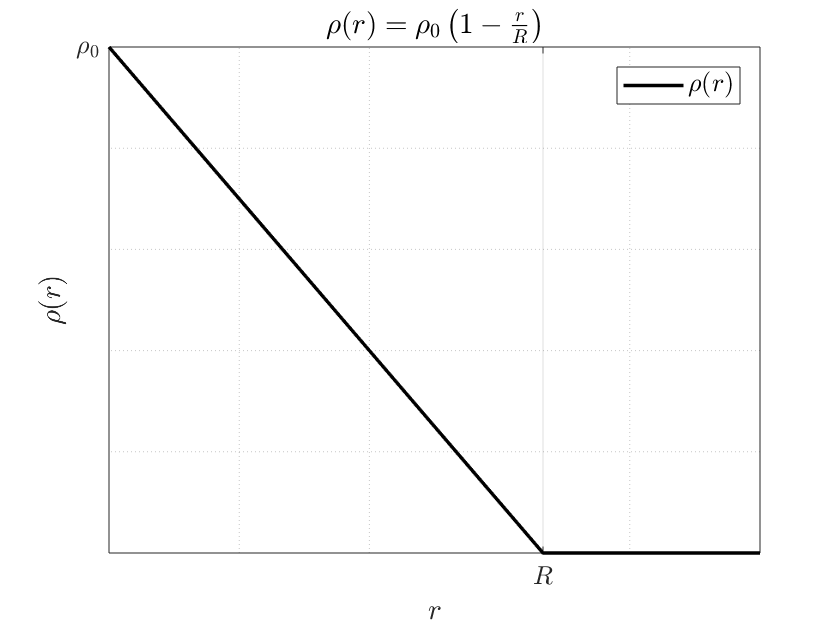
\includegraphics[width=.6\textwidth]{Astrofysik/billeder/PlanetMasse.png}
	\caption{Tegning af funktionen $\rho(r)$ for $r\geq0$.}
	\label{fig:PlanetMasse}
\end{figure}
%
%
\begin{opgave}{Masse af en planet}{2}
\opg Se figur \ref{fig:PlanetMasse}.
\opg Funktionen indsættes i integralet, som derefter løses
\begin{align*}
    M = 4\pi\int_0^R\rho(r)r^2\d r = 4\pi\rho_0\int_0^R r^2 - \frac{r^3}{R} \d r = 4\pi\rho_0 \left[\frac{1}{3}r^3 - \frac{r^4}{4R}\right]_0^R = 4\pi\rho_0 \left[\frac{1}{3}R^3 - \frac{1}{4}R^3\right] = \frac{1}{3}\pi\rho_0R^3 \: .
\end{align*}
\end{opgave}
%
%
\begin{opgave}{Tyngdeaccelerationen indeni en planet}{3}
\opg Densitet har enheden \si{\kilo\gram\per\metre\cubed}, mens $r$ har enheden \si{\metre}, hvorfor
\begin{align*}
    [A] = [\rho r^2] = \si{\kilo\gram\per\metre} \: .
\end{align*}
\opg For at forstå sådanne funktioner kan det være værd at kigge på hvilket dele af funktionen, der er størst i hvilke områder: \\
-- \; $\lim\limits_{r\rightarrow0}(1/r^2) = \infty$, mens $\exp(-R/c) < \infty$, hvorfor $1/r^2$ dominerer for små $r$. Ergo opfører $\rho(r)$ sig som $1/r^2$ for små værdier af $r$. \\
-- \; Eksponentialfunktionen er aftagende idet eksponenten er negativt på hele definitionsmængden, hvorfor den kun bliver dominerende, hvis den aftager tilpas meget langsommere end $1/r^2$. Jo mindre $c$ bliver, desto større bliver $(r-R)/c$, hvorfor eksponentialfunktionen dominerer mest for små værdier af $c$. Eksponenten går mod 0, for $r \rightarrow R$ uanset hvad $c$ er, hvorfor betydningen af $c$ må blive mindre jo større $r$ bliver. \\
-- \; Planetens radius er $R$, hvorfor $\rho(r) = 0$ for $r>R$, hvilket ses ved at funktionen brat går i nul og bliver der. \\
-- \; Af figurens ses det at $\rho(r) \xrightarrow{r\rightarrow0} \infty$ uanset hvad værdien af $c$ er. \\
-- \; Det ses også at $\rho(r)$ først begynder at afvige drastisk fra $1/r^2$, når $c<0,5$. For alle værdier af $c$ bliver grafen godt nok næsten flad eller voksende når $r$ nærmer sig $R$, men det sker meget sent for de største værdier af $c$. \\
-- \; For de mindste værdier af $c$ bliver eksponenten så stor at den meget hurtigt begynder at dominere, hvorfor $1/r^2$ delen kun ses for meget små $r$. \\ \\
-- \; Alt i alt er størstedelen af planetens masse samlet tæt på centrum, og interessant nok er der ikke ret meget masse omkring $r = R/2$, hvis $c$ er tilpas lille. \\
-- \; Hvorvidt denne funktion overhoved kan modellere massen af en planet skal være usagt, men som teoretisk eksempel er den ganske interessant.
\opg Det er bare integralets grænse, der skal ændres, og formelt set bør man også ændre integrationsvariablen så
\begin{align*}
    M(r) = \int_0^r\rho(r')4\pi (r')^2\d r' \: .
\end{align*}
\opg Nu er det bare at kombinere formlerne og løse integralet.
\begin{align*}
    g(r) &= \frac{G}{r^2}\int_0^r\rho(r')4\pi (r')^2\d r' = \frac{4\pi G}{r^2}\int_0^r\frac{A}{(r')^2}\exp\left(\frac{r'-R}{c}\right)4\pi(r')^2\d r' \\[1mm]
    &= \frac{4\pi AG}{r^2}\int_0^r\exp\left(\frac{r'-R}{c}\right) \d r' \: .
\end{align*}
For at løse dette integral benyttes en substitution
\begin{align*}
    u = \frac{r'-R}{c} \Rightarrow \dif{r'}{u} = \frac{1}{c} \Rightarrow \d r' = c\d u \: .
\end{align*}
Yderligere skal grænserne ændres
\begin{align*}
    u(0) = -\frac{R}{c} \quad , \quad u(r) = \frac{r-R}{c} \: ,
\end{align*}
hvorved det substituerede integral bliver
\begin{align*}
    g(r) = \frac{4\pi AG}{r^2} \int_{-R/c}^{(r-R)/c} \exp\left(u\right)c \d u = \frac{4\pi cAG}{r^2} \bigg[\exp(u)\bigg]_{-R/c}^{(r-R)/c} = \frac{4\pi cAG}{r^2} \left[\exp\left(\frac{r-R}{c}\right) - \exp\left(-\frac{R}{c}\right)\right] \: .
\end{align*}
\end{opgave}
\chapter{Atom- og Molekylefysik}
\begin{opgave}{Finstruktur for en elektron}{1}
Vi vil i denne opgave se på tilstanden n=2 for hydrogenatomet.
\opg For $s=\frac{1}{2}$ l=1, udregn $\beta_l$
$$\beta_1=\frac{g_s1^3e^8m_e}{c^22^3\hbar^44^5\pi^4\epsilon_0^4}\frac{1}{1(1+0.5)(1+1)}$$
\opg Find alle værdier af J for n=2 tilstanden.
$$J=|l+s|,|l+s-1|,..,|l-s|$$
hvilket giver $J=\frac{3}{2},\frac{1}{2}$
\opg Find energi opsplitningen for tilstandende n=2,l=0.
$$\left<\hat{s}\cdot\hat{l}\right>=\frac{1}{2}(j(j+1)-l(l+1)-s(s+1))$$
hvis l=0, er j=s, hvilket giver:
$$\left<\hat{s}\cdot\hat{l}\right>=\frac{1}{2}(j(j+1)-s(s+1))=0$$
dvs. for l=0 $H_{s-o}=0$
\opg Find energi opsplitningen for tilstandende n=2,l=1.
$$\left<\hat{s}\cdot\hat{l}\right>=\frac{1}{2}(j(j+1)-l(l+1)-s(s+1))$$
for $j=\frac{3}{2}$
$$\left<\hat{s}\cdot\hat{l}\right>=\frac{1}{2}(\frac{3}{2}(\frac{3}{2}+1)-1(1+1)-\frac{1}{2}(\frac{1}{2}+1))=\frac{1}{2}(\frac{15}{4}-\frac{8}{4}-\frac{3}{4})=\frac{1}{2}$$
for $j=\frac{1}{2}$
$$\left<\hat{s}\cdot\hat{l}\right>=\frac{1}{2}(\frac{1}{2}(\frac{1}{2}+1)-1(1+1)-\frac{1}{2}(\frac{1}{2}+1))=\frac{1}{2}(-1(1+1))=-1$$
dvs. at energiforskellen er givet ved:
$\Delta E=E_{j=\frac{3}{2}}-E_{j=\frac{1}{2}}=\frac{\beta_1}{2}-(-\beta_1)=\frac{3}{2}\beta_1$
\end{opgave}
\begin{opgave}{Finstruktur for flere elektroner}{3}
Vi vil i denne opgave se på et system med 2 elektronerhvor de hver har n=2.
\opg Find alle L og S værdier for $l_1=1$ og $l_2=1$,hvorfor er det ikke nødvendigt at specificere hvad $s_1$ og $s_2$ er?\\
\\
Der er ikke nødvendigt at specificere hvad $s_1$ og $s_2$ er, da elektroner er fermioner og de har pr. definitions altid spin $\frac{1}{2}$
$$L=|l_1+l_2|,|l_1+l_2-1|,..,|l_1-l_2|$$
hvilket giver $L=2,0$
$$S=|s_1+s_2|,|s_1+s_2-1|,..,|s_1-s_2|$$
hvilket giver $S=1,0$
\opg Find alle J værdier for L og S fra forrige opgave.
$$J=|L+S|,|L+S-1|,..,|L-S|$$
Her skal man kombinere begge værdier af L med begge værdier af S, hvilket giver:\\
$J=3,2,1,0$
\opg Find alle energiopsplitningerne for de J, L og S tilstande vi fandt i de forrige opgaver.\\
Her skal vi først tænke os om. Den eneste måde vi kan få
\end{opgave}
\begin{opgave}{Hyperfinstruktur for 21 cm linjen}{1}
Vi vil i denne opgave arbejde med den hyperfinestruktur for en elektron i grundtilstanden af et brin-tatom.
\opg Kernen er en proton med spin $\frac{1}{2}$, find alle værdier af F. Hvorfor er det ikke nødvendigt at kende $l$ for elektronen?\\
Da vi arbejder med grundtilstanden er $l=0$, altid!.\\
$J,I=\frac{1}{2}$, dvs:
$$F=|J+I|,|J+I-1|,..,|J-I|$$
Hvilket giver F=1,0.
\opg Udregn konstanten A for grundtilstanden.
 Bemærk at $g_I = 5,58569468$
$$A=\frac{2}{3}\mu_0g_s\mu_Bg_I\mu_N\frac{Z^3}{\pi a_o^3}=\SI{9,428e-25}{J} =$$
\opg Find energiopsplitningen mellem tilstandende.\\
Da energien er givet ved $E=A\left<\hat{J}\cdot\hat{I}\right>$, får vi energien for de to forskellige tilstande af F til:\\
For F=1
$$\left<\hat{J}\cdot\hat{I}\right>=\frac{1}{2}(1(1+1)-\frac{1}{2}(\frac{1}{2}+1)-\frac{1}{2}(\frac{1}{2}+1))=\frac{1}{2}(\frac{1}{2})=\frac{1}{4}$$
så $E_{F=1}=\frac{A}{4}$\\
For F=0
$$\left<\hat{J}\cdot\hat{I}\right>=\frac{1}{2}(0(0+1)-\frac{1}{2}(\frac{1}{2}+1)-\frac{1}{2}(\frac{1}{2}+1))=\frac{1}{2}(\frac{-6}{4})=\frac{-3}{4}$$
$E_{F=0}=\frac{-3}{4}A$
Energiforskellen mellem de to tilstande bliver derfor:
$$\Delta E=E_{F=1}-E_{F=0}=\frac{1}{4}A-\frac{-3}{4}A=A$$
\opg Udregn bølgelængden af det lys som har en energi svarende til energiforskellen mellem de to tilstande.
$$E_{lys}=h\cdot f$$
$$c=\lambda\cdot f$$
så:
$$E_{lys}=\frac{h\cdot c}{\lambda}=A$$
Hvilket giver:
$$\lambda=\frac{h\cdot c}{A} = \SI{21,07}{cm}$$
\end{opgave}
\begin{opgave}{Hyperfinstruktur for atomure}{2}
Vi vil i denne opgave arbejde med et cæsium atom, som det er beskrevet i teksten.
Spinnet for et cæsium kerne er I=$\frac{7}{2}$ og vi vil i denne opgave arbejde med n=6 tilstanden.
\opg Find alle F tilstande for l=0.\\
$$F=|J+I|,|J+I-1|,..,|J-I|$$
Hvilket giver F=4,3.
\opg Udregn energiopsplitningen for tilstandende.\\
For F=4
$$\left<\hat{J}\cdot\hat{I}\right>=\frac{1}{2}(4(4+1)-\frac{7}{2}(\frac{7}{2}+1)-\frac{1}{2}(\frac{1}{2}+1))=\frac{7}{4}$$
For F=3
$$\left<\hat{J}\cdot\hat{I}\right>=\frac{1}{2}(3(3+1)-\frac{7}{2}(\frac{7}{2}+1)-\frac{1}{2}(\frac{1}{2}+1))=\frac{-9}{4}$$
Dvs. at energiforskellen mellem tilstandene er:
$$\Delta E=E_{F=4}-E_{F=3}=\frac{7}{4}A_n-\frac{-9}{4}A_n=4A_n$$
Da $A_n=A_1\frac{1}{n^3}$ så da n=6 får vi den samlede energiforskel til at være:
$$\Delta E=\frac{4}{6^3}A_1$$
Hvor $A_1$ er værdien af A vi fandt i opgaven om hyperfin opsplitningen for grundtilstandsenergien.
\opg Udregn frekvensen af det lys der bliver udsendt fra denne overgang.
$$E_{lys}=h\cdot f=\Delta E$$
$$\frac{4}{6^3}A_1=h\cdot f$$
$$f=\frac{4}{6^3}\frac{A_1}{h}$$
\end{opgave}
\begin{opgave}{Diatomare molekyler}{1}
\begin{figure}[h]
\center
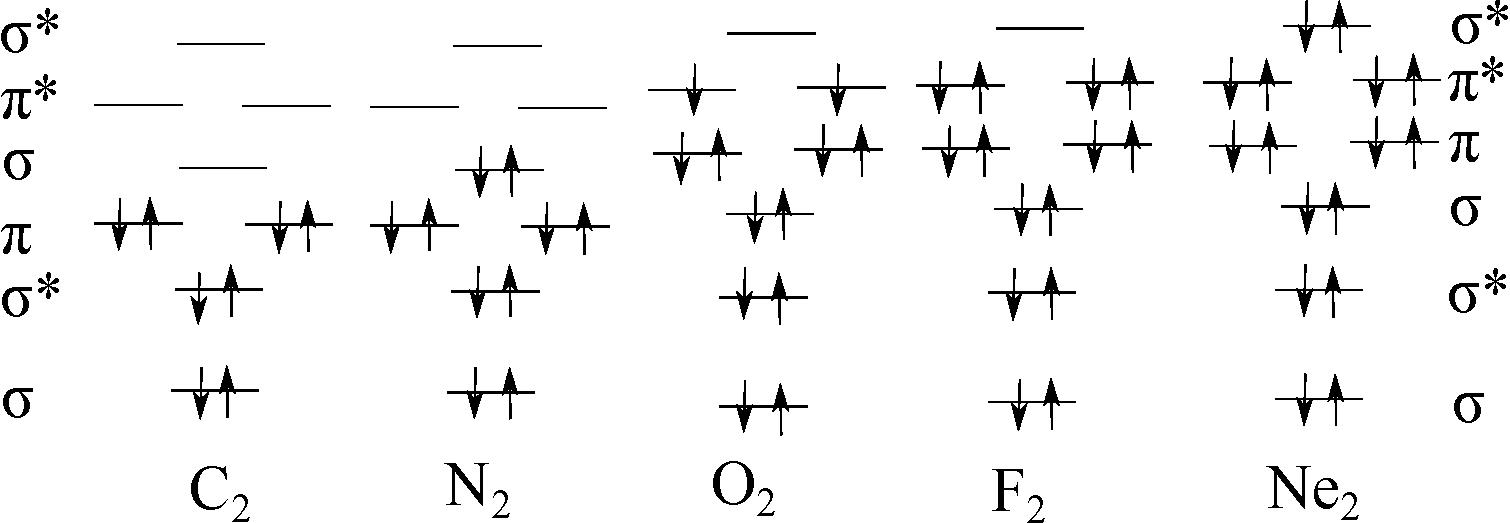
\includegraphics[width = \textwidth]{Atom-ogMolekylefysik/billeder/diatomar.pdf}
\caption{Molekyleorbitaldiagrammer of diatomare molekyler.}
\label{opg:diatomar}
\end{figure}
\opg Diatomare molekyler lettere end N$_2$ har samme struktur af orbitaler som N$_2$. De tungere har samme struktur som O$_2$.
\opg Bindingsorden er antallet af fyldte bindende orbitaler minus antallet af fyldte antibindende orbitaler, så:
\begin{tabular}{c|c c c c c}
&C$_2$&N$_2$&O$_2$&F$_2$&Ne$_2$\\\hline
$b$&2&3&2&1&0
\end{tabular}
\opg N$_2$ vil være det mest ustabile, da det har den laveste bindingsorden, og ganske rigtigt Findes Ne$_2$ ikke. C$_2$ forekommer hellerikke, men det er fordi kulstof kan danne andre strukturer så som diamant og grafit, der er mere stabile.
\opg Kun O$_2$ har uparrede elektroner, så det er det eneste af molekylerne der er magnetisk.
\end{opgave}
\begin{opgave}{Vand}{2}
\opg Brintmolekylet har den bindende og den anti bindende $\sigma$ orbital.
\begin{figure}[h]
\center
\includegraphics[width = \textwidth]{Atom-ogMolekylefysik/billeder/tilstande1.pdf}
\end{figure}
\opg
Det frie ilt har $1s$, $2s$ og $2p$ orbitalerne, men $1s$ ligger meget lavere end de andre og indgår ikke i bindingen.
\begin{figure}[h]
\center
\includegraphics[width = \textwidth]{Atom-ogMolekylefysik/billeder/tilstande2.pdf}
\end{figure}
\opg
Lægges bindingsaksen for H$_2$ langs $y$-aksen og føres ind imod O-atomet langs $z$-aksen. Så vil orbitalerne overlappe hvis de kan have fælles fortegn i hele kontaktområdet. Det betyder at $p_x$ ikke overlapper med nogle da den kan en knudeflade i $yz$-planen, som ingen andre orbitaler har. $p_y$ overlapper med $\sigma^*$. Derudover overlapper $\sigma$ med både $s$ og $p_z$.
\opg For at opstille molekyleorbitaldiagrammet ser man på tabel 4.1 for energien af O orbitalerne. H$_2$ orbitalerne er en slat lavere end $1s$ for brintatomet, for $\sigma$ og højere for $\sigma^*$.
$p_x$ forbliver uændret, da den ikke har noget overlap. 
$\sigma^*$ og $p_y$ viser sig at give en stor opsplitning. Disse orbitaler kaldes af grunde vi desværre ikke var i stand til at dække $1b_2$ og $2b_2$. De spøjse navne stammer fra en måde at kategorisere molekylers symmetri, baseret på gruppeteori.
De sidste tre orbitaler har en hævet, en imidten og en lav. disse kaldes $4a_1$, $3a_1$ og $2a_1$. På figuren kalds den uændrede $p_x$-orbital også for $b_1$

Det vigtige er at vide hvilke orbitaler der interagerer og hvordan det fører til opsplitning, graden af opsplitning er ikke super essentiel, da det ikke er muligt at udregne med de værktøjer vi har præsenteret her.

Elektroner indsættes efter Aufbau princippet nedefra.
\begin{figure}[h]
\center
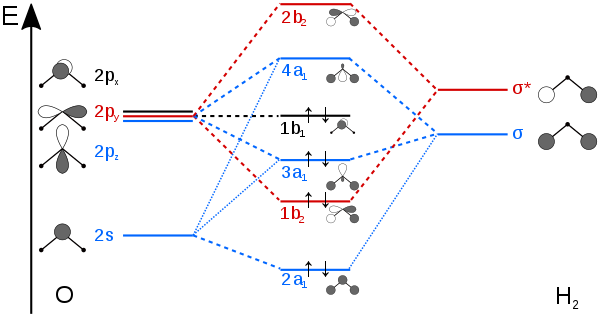
\includegraphics[width = \textwidth]{Atom-ogMolekylefysik/billeder/H2O-MO-Diagram-wiki.png}
\caption{Molekyleorbitaldiagrammet for vand.}
\end{figure}
\opg At afgøre om orbitaler er bindende, antibindende eller ikke bindende er ikke helt så simpelt som for homoatomare diatomiske molekyler, men det gøres lettest ved at sammenligne hver orbital med de tilsvarende i det ubundne molekyle. Det giver at de to nederste to orbitaler, $2a_1$ og $1b_2$, er bindende, $3a_1$ og $1b_1$ er ikke bindende og $4a_1$ og $2b_2$ er antibindende.
\opg Der er to fyldte bindende orbitaler og to ikke bindende, så bindingsordenen er 2, svarende til to enkeltbindinger.
\end{opgave}
\begin{opgave}{Benzen}{3}
\opg Index viser hvor langt rundt langs ringen det tilhørende atom er, så $p_7$ svarer til $p_1$. 
\opg $p$-orbitalerne giver allerede en knudeflade i ringens plan. Ønskes så få som muligt vil alle $p$ orbitalerne med samme fortegn give ingen nye knudeflader.
$$
1\pi = \sum_{i=1}^6 p_i = p_1+p_2+p_3+p_4+p_5+p_6
$$
\opg
Gives de alternerende forgen kommer der tre knudeflader imellem alle atomerne.
$$
6\pi = \sum_{i=1}^3 (p_{2i}-p_{2i+1})=p_1+p_2+p_3-p_4+p_5-p_6
$$
\begin{figure}
\center
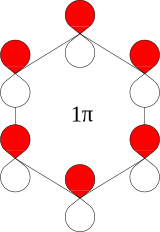
\includegraphics[width = 0.45\textwidth]{Atom-ogMolekylefysik/billeder/benzen1}
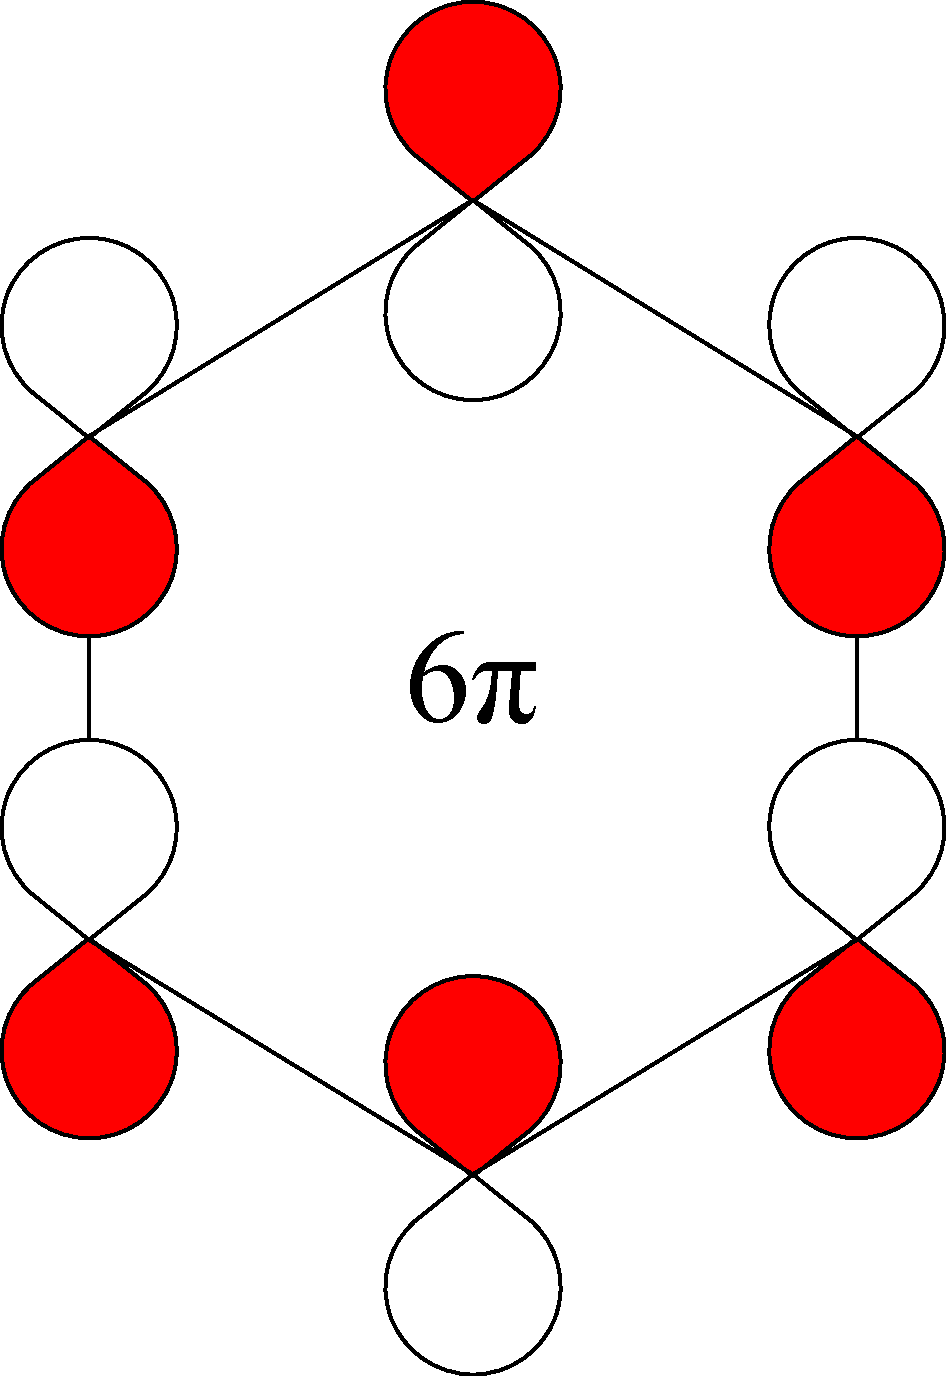
\includegraphics[width = 0.45\textwidth]{Atom-ogMolekylefysik/billeder/benzen6}
\caption{De to tilstande $1\pi$(til venstre) og $6\pi$(til højre).}
\end{figure}
\opg For $1\pi$ er sum notation et godt værktøj.
\begin{align*}
\op H 1\pi &= \op H \sum_{i=1}^6\\
&= \sum_{i=1}^6 \op Hp_i\\
&= \sum_{i=1}^6 (\alpha p_i+\beta p_{i-1}+\beta p_{i+1})\\
&= \sum_{i=1}^6 \alpha p_i+\sum_{i=1}^6\beta p_{i-1}+\sum_{i=1}^6\beta p_{i+1}\\
&= \alpha \sum_{i=1}^6 p_i+2\beta \sum_{i=1}^6 p_i\\
&= (\alpha +2\beta)1\pi
\end{align*}
Så energien er:
$$
E=\alpha + 2\beta
$$
For $6\pi$ har vi:
\begin{align*}
\op H 6\pi &= \op H \sum_{i=1}^3 (p_{2i}-p_{2i+1})\\
&=\sum_{i=1}^3 (\alpha p_{2i}+\beta p_{2i-1}+\beta p_{2i+1}-\alpha p_{2i+1}-\beta_{2i}-\beta p_{2i+2})\\
&= \alpha \sum_{i=1}^3 (p_{2i}-p_{2i+1})+\beta\sum_{i=1}^3(p_{2i-1}+p_{2i+1}-p_{2i}-p_{2i+2})\\
&=\alpha 6\pi+\beta\sum_{i=1}^3(p_{2i-1}-p_{2i})+(p_{2i+1}-p_{2i+2})\\
&=\alpha6\pi-\beta\left(\sum_{i=1}^3(p_{2i}-p_{2i-1})+\sum_{i=1}^3(p_{2i+2}-p_{2i+1}\right)\\
&= (\alpha-2\beta)6\pi
\end{align*}
Så energien er:
$$
\alpha-2\beta
$$
\opg $1\pi$ skal have den mindste energi, så $\beta$ må være negativ.
\opg
Der er fejl i denne opgave, første $2\pi$ skulle have været:
$$
2\pi = \frac{1}{2\sqrt{3}}\left(2p_1+p_2-p_3-2p_4-p_5+p_6\right)
$$
Desuden skulle den anden  $2\pi$ have været $4\pi$ \& anden $3\pi$ have været $5\pi$.
\begin{figure}[h]
\center
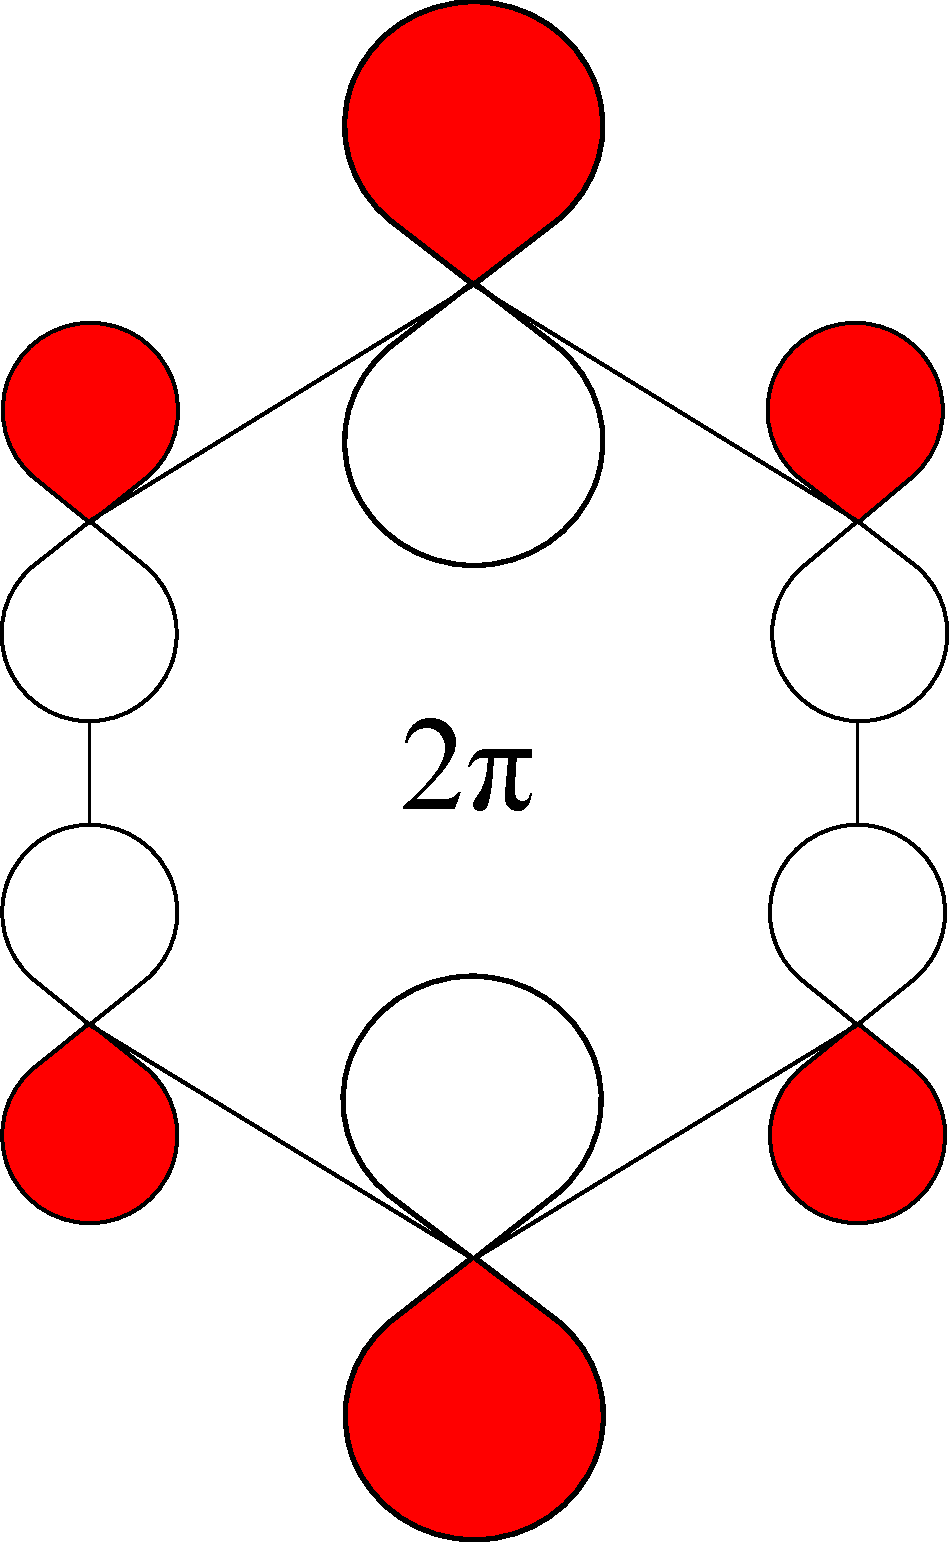
\includegraphics[width = 0.35\textwidth]{Atom-ogMolekylefysik/billeder/benzen2.pdf}
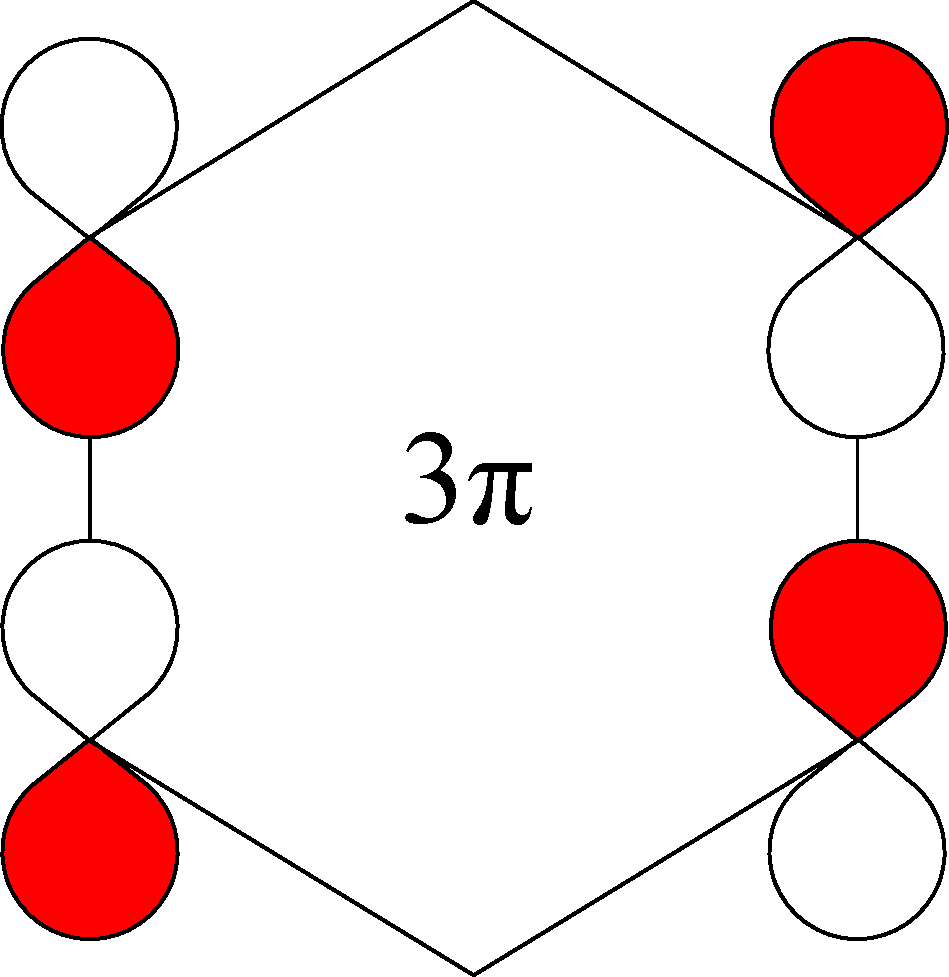
\includegraphics[width = 0.35\textwidth]{Atom-ogMolekylefysik/billeder/benzen3.pdf}
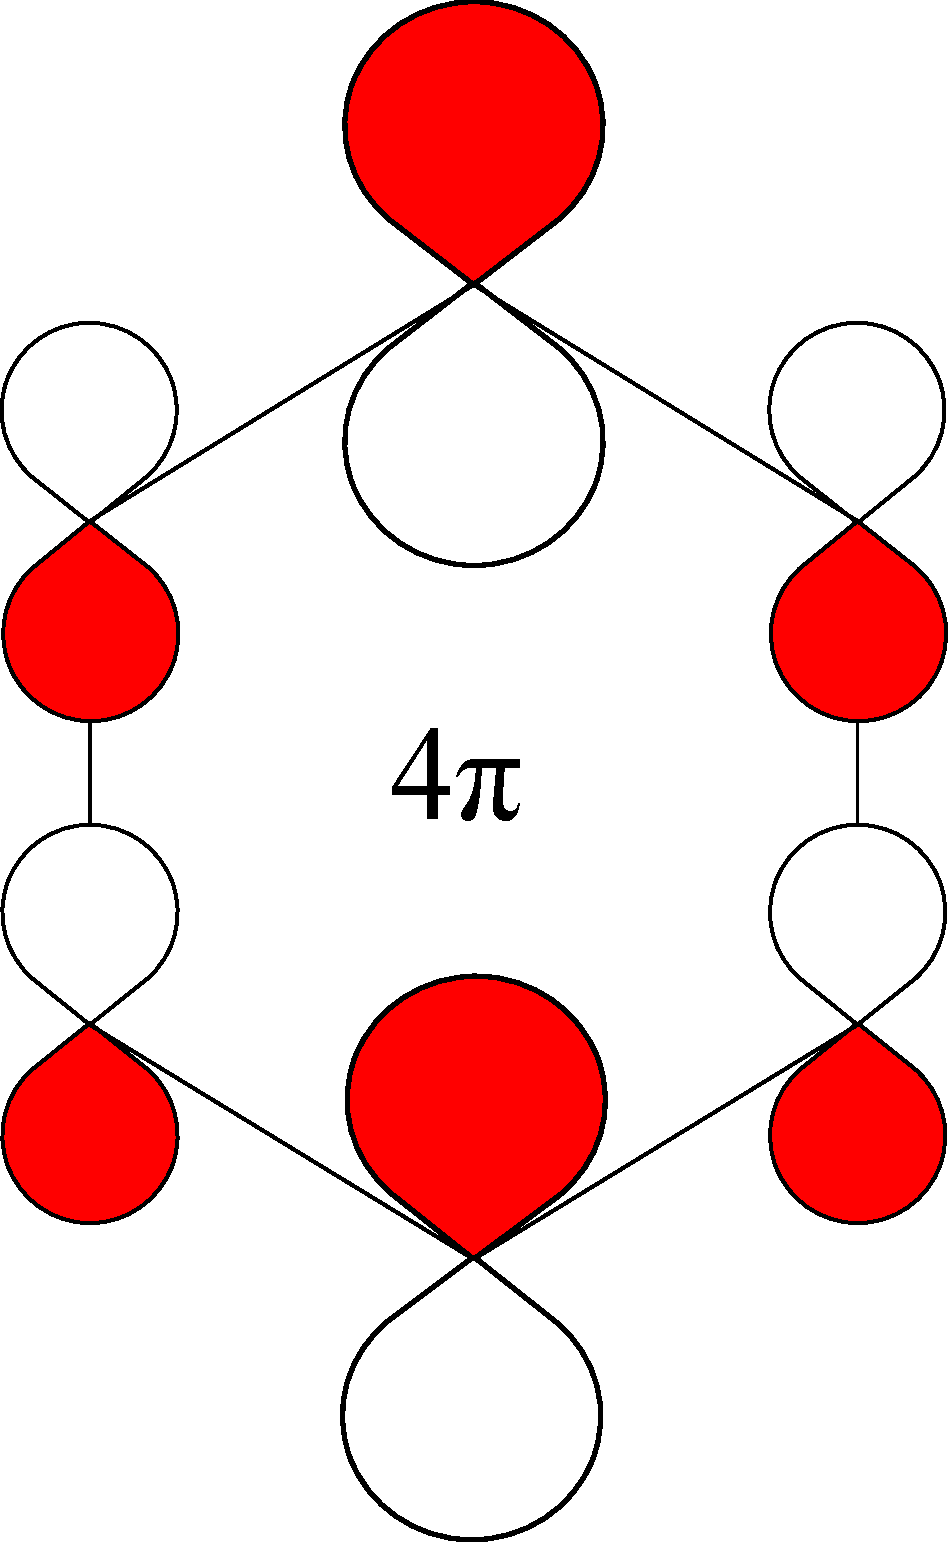
\includegraphics[width = 0.35\textwidth]{Atom-ogMolekylefysik/billeder/benzen4.pdf}
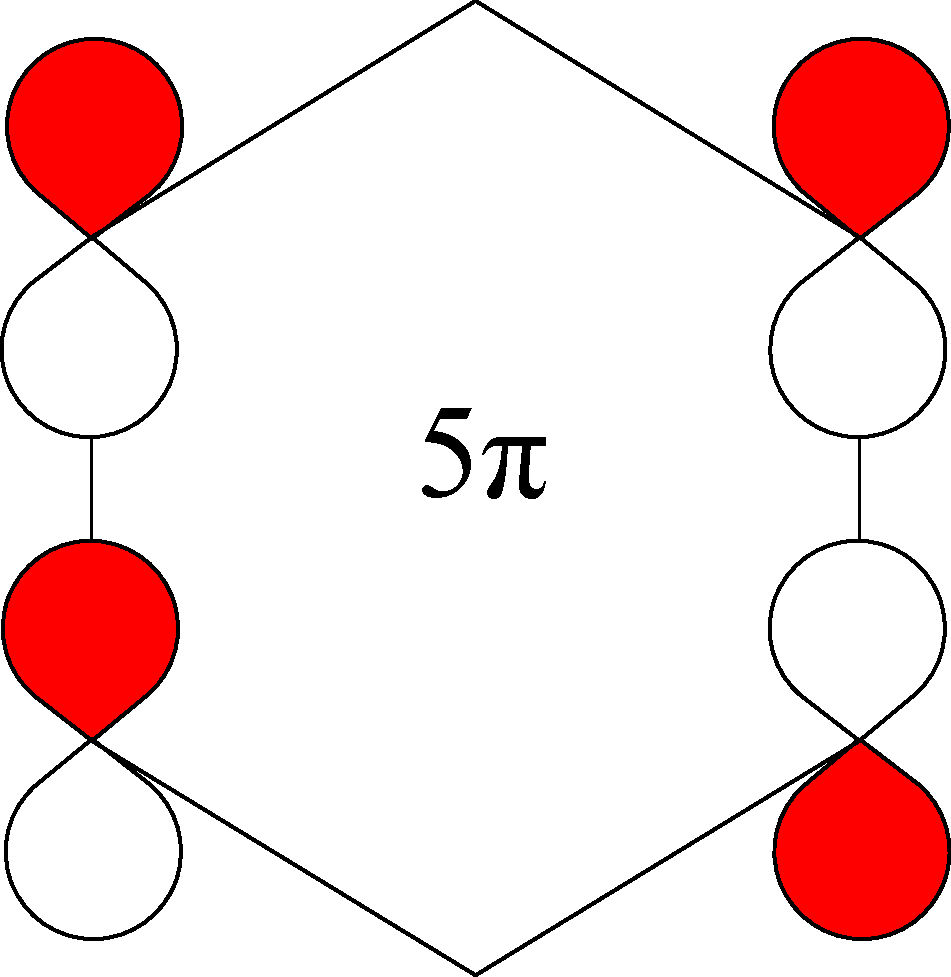
\includegraphics[width = 0.35\textwidth]{Atom-ogMolekylefysik/billeder/benzen5.pdf}
\caption{Skitser af de fire mellemste $\pi$-orbitaler}
\end{figure}
\opg
For at opstille molekyleorbitaldiagrammet er det nødvendigt at kende de sidste bølgefunktioners energi. Energien findes ved at anvende Hamiltonoperatoren på de fire tilstande.
\begin{align*}
\op H 2\pi &= \op H \frac{1}{2\sqrt{3}}(2p_1+p_2-p_3-2p_4-p_5+p_6)\\
&= \frac{1}{2\sqrt{3}}(\alpha(2p_1+p_2-p_3-2p_4-p_5+p_6)+\beta(2p_6+p_1-p_2-2p_3-p_4+p_5)+\beta(2p_2+p_3-p_4-2p_5-p_6+p_1))\\
&=\frac{1}{2\sqrt{3}}(\alpha(2p_1+p_2-p_3-2p_4-p_5+p_6)+\beta(2p_1+p_2-p_3-2p_4-p_5+p_6)\\
&=(\alpha+\beta)2\pi\\
\op H 3\pi &= \op H\frac{1}{2} (2p_2+p_3-p_5-p_6)\\
&= \frac{1}{2}(\alpha((2p_2+p_3-p_5-p_6)+\beta((2p_1+p_2-p_4-p_5)+\beta((2p_3+p_4-p_6-p_1))\\
&=\frac{1}{2}(\alpha(2p_2+p_3-p_5-p_6)+\beta(2p_2+p_3-p_5-p_6)\\
&=(\alpha+\beta)3\pi\\
\op H 4\pi &= \op H \frac{1}{2\sqrt{3}}(2p_1-p_2-p_3+2p_4-p_5-p_6)\\
&=\frac{1}{2\sqrt{3}}(\alpha(2p_1-p_2-p_3+2p_4-p_5-p_6)+\beta(2p_6-p_1-p_2+2p_3-p_4-p_5)+\beta(2p_2-p_3-p_4+2p_5-p_6-p_1))\\
&=\frac{1}{2\sqrt{3}}(\alpha(2p_1-p_2-p_3+2p_4-p_5-p_6)+\beta(-2p_1+p_2+p_3-2p_4+p_5+p_6))\\
&=(\alpha-\beta)4\pi\\
\op H 5\pi &= \op H\frac{1}{2}(p_2-p_3+p_5-p_6)\\
&= \frac{1}{2}(\alpha(p_2-p_3+p_5-p_6)+\beta(p_1-p_2+p_4-p_5)\beta(p_3-p_4+p_6-p_1))\\
&= \frac{1}{2}(\alpha(p_2-p_3+p_5-p_6)+\beta(-p_1+p_2-p_5+p_6))\\
&=(\alpha-\beta)5\pi
\end{align*}
Nu hvor vi kender energien kan vi opstille et molekyleorbitaldiagram.
\begin{figure}[h]
\center
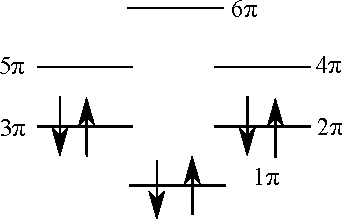
\includegraphics[width = \textwidth]{Atom-ogMolekylefysik/billeder/benzenMO.pdf}
\caption{Molekyleorbitaldiagram for benzens $\pi$ system.}
\end{figure}
\end{opgave}
\begin{figure}[t]
	\centering
	%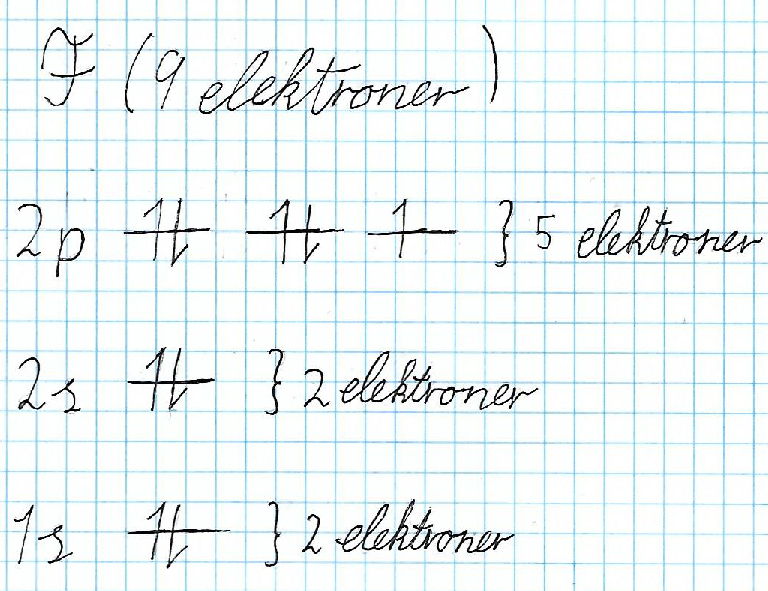
\includegraphics[width=\columnwidth]{Atom-ogMolekylefysik/billeder/F.pdf}
	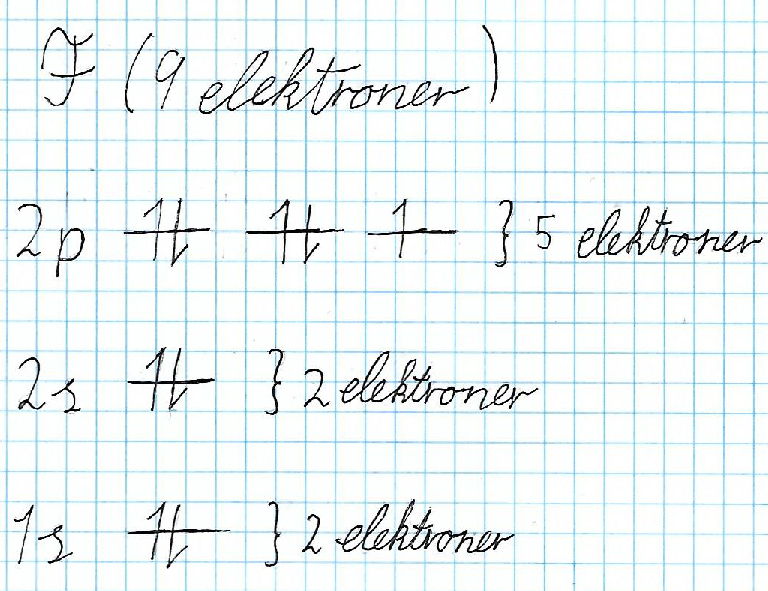
\includegraphics[width=\columnwidth]{Atom-ogMolekylefysik/billeder/F.pdf}
	\caption{Elektronstrukturen for F.} \label{fig:F}
\end{figure}
\begin{figure}[t]
	\centering
	%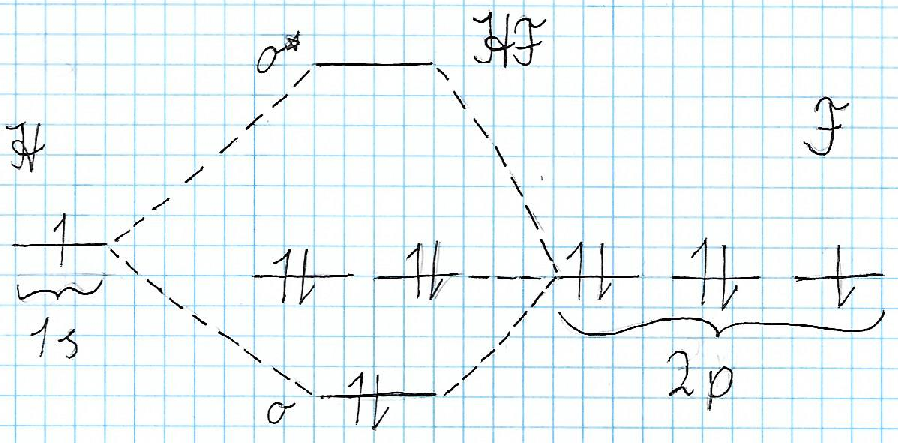
\includegraphics[width=\columnwidth]{Atom-ogMolekylefysik/billeder/HF.pdf
	\includegraphics[width=\columnwidth]{Atom-ogMolekylefysik/billeder/HF.pdf}
	\caption{Elektronstrukturen for HF, hvor de to midterste er ikke-bindende $p$-orbitaler. Bemærk at $\sigma^*$-orbitalen er tom, samt at alle elektronerne befinder sig i en tilstand med samme eller lavere energi end før.} \label{fig:HF}
\end{figure}
\begin{figure}[t]
	\centering
	%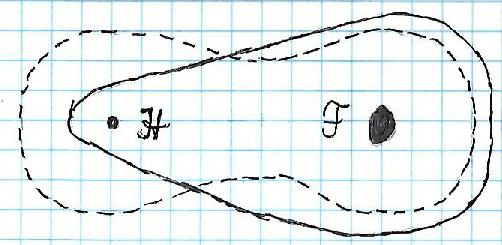
\includegraphics[width=\columnwidth]{Atom-ogMolekylefysik/billeder/HF_orbit.pdf}
	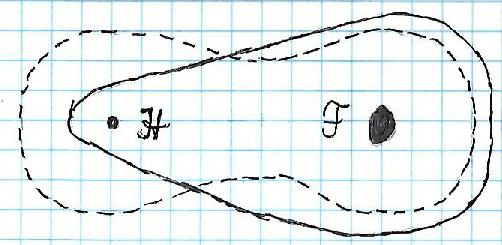
\includegraphics[width=.9\columnwidth]{Atom-ogMolekylefysik/billeder/HF_orbit.pdf}
	\caption{Skitse den bindende $sigma$-orbital for HF, hvor den stiplede linje indikerer hvordan den ville se ud, hvis man ikke tager højde for forskellene mellem H og F, mens den fuldtoptrukne tager denne forskel i betragtning.} \label{fig:HF_orbit}
\end{figure}
\begin{opgave}{Halogener og hydrogenbindinger}{3}
\opg Se figur \ref{fig:F}
\opg Fra forgående spørgsmål ses det at flour mangler 1 elektron for at have sin yderste $p$-orbital fuld, og dermed opnå den stabile tilstand af en fuld yderste $s$- og $p$-orbital, hvilket gælder for alle halogenerne.
\opg De to $s$-orbitaler deltager ikke i bindingen, hvorfor de ikke tegnes. I figur \ref{fig:HF} ses det at elektronerne er i en lavere energitilstand, hvis de to atomer bindes til hinanden, end hvis de holder sig hver for sig.
\opg Bindingen er en $\sigma$-binding, da den er mellem en $s$- og en $p$-orbital.
\opg Hydrogen findes ofte som ${}^1$H, hvilket vil sige at det består af en proton og en elektron, men ingen neutroner. En proton er stabil som sig selv, mens flour meget gerne vil have en elektron til at fylde sin sidste $p$-orbital. Flour trækker derfor meget mere i $\sigma$-orbitalen end hydrogen, hvilket forskyder orbitalen mod flour, som illustreret i figur \ref{fig:HF_orbit}.
\opg Eftersom H i gennemsnit "mangler" sine elektroner, er det en "åben proton". Der er ikke noget, der skærmer den i retningen væk fra flour, hvorfor den tiltrækker alt hvad der er negativt. Det gælder både det flouratom, den er bundet til, hvorfor bindingslængden er ekstremt kort, men det gælder også flouratomer i andre HF-molekyler. Derfor tiltrækker den negative del af et HF-molekyle den positive del af et andet HF-molekyle, hvilket er hvad der kaldes en hydrogenbinding. I nogle tilfælde er hydrogenbindingen faktisk så stærk, at orbitalerne fra to tilstødende molekyler begynder at overlappe, hvilket gør at båndet får kovalent karakter, fremfor at opføre sig rent som en intermolekylær kraft.
\opg Tages chlor som eksempel, så er $Cl$ grundstof nummer 17, hvilket betyder at orbitalerne $1s$, $s2$, $2p$ og $3s$ er fyldte, mens det er $3p$-orbitalen, der mangler en elektron, for at være fuld. Det betyder at der er markant flere elektroner omkring chlor, og elektroner frastøder hinanden, hvorfor chlor ikke kan trække så meget i det bindende elektronpar. Man siger at kernen er skærmet og har en mindre effektiv kerneladning. Chloratomet kan derfor ikke trække elektronparet ligeså tæt på sig som flour kan, og det befinder sig derfor tættere på H. Derudover kommer H ikke så tæt på Cl, som det kan komme på F, hvorfor ladningsforskydningen eller dipolmomentet ikke er stort nok til at danne hydrogenbindinger. Da både brom og iod er større end chlor gælder dette også for dem. Det er netop det at $\mathrm{HF}(aq)$ er så svært at styrre, og det forklarer også hvorfor de andre hydrogenhalider er stærkere syrer end flussyre.
\end{opgave}
\section*{Spin}
\begin{opgave}{Pauli princippet uden spin}{1}
Lad $\op O$ være ombytningsoperatoren. Som navnet antyder er det den operator, der får to elektroner til at bytte plads:
$$
\op O \Psi(x_1,x_2) = \Psi(x_2,x_1)
$$
Lad $\psi(x)$ være en én elektron tilstand, og $\Psi(x_1,x_2) = \psi(x_1)\psi(x_2)$.
\opg Hvad er $\op \Psi(x_1,x_2)$?\\
For at en tilstand kan opfylde Pauli princippet, skal bølgefunktionen være antisymmetrisk under ombytning. Det vil sige $\Psi(x_1,x_2) = -\Psi(x_2,x_1)$.
\opg Er $\Psi(x_1,x_2)$ tilladt ifølge Pauli?
\end{opgave}
%
\begin{opgave}{Rumbølgefinktioner}{2}
Lad os i stedet se på to elektroner i to forskellige tilstande $\psi_1$ og $\psi_2$. Her indikerer subscriptet på $\psi$ tilstanden, men subscripts på $x$ angiver hhv. elektron 1 og 2.\\
Lad nu
\begin{align*}
\Psi_{12}(x_1,x_2) &= \psi_1(x_1)\psi_2(x_2) \, , \\
\Psi_{21}(x_1,x_2) &= \psi_2(x_1)\psi_1(x_2) \, .
\end{align*}
Udregn de følgende ombytninger.
\opg $\op O \Psi_{12}(x_1,x_2)$.
\opg $\op O \Psi_{21}(x_1,x_2)$.
\opg $\op O \Psi^S(x_1,x_2)=\op O (\Psi_{12}(x_1,x_2)+\Psi_{21}(x_1,x_2))$.
\opg $\op O \Psi^A(x_1,x_2)=\op O (\Psi_{12}(x_1,x_2)-\Psi_{21}(x_1,x_2))$.
\opg Er bølgefunktionerne symmetriske, antisymmetriske eller ingen af delene.
\end{opgave}
%
\begin{opgave}{Pauli med spin}{3}
Nu vil vi tage højde for spin. Det gøres ved at multiplicere bølgefunktionen med en spinfunktion. Elektronen kan have spin op eller spin ned. Det angives med $\alpha$ eller $\beta$. For at holde styr på hvilken partikel der har hvilket spin tilføjes et tal til spinfunktionen. Så har partikel 1 spin op og partikel 2 spin ned skrives det: $\chi=\alpha(1)\beta(2)$.
Ombytningsoperatoren ombytter også, hvilken partikel der har hvilket spin.
Hvad er:
\opg $\op O \alpha(1)\alpha(2)$.
\opg $\op O \beta(1)\beta(2)$.
\opg $\op O \alpha(1)\beta(2)$.
\opg $\op O \beta(1)\alpha(2)$.
\opg Brug dette til at finde tre spinfunktioner, der er symmetriske under ombytning.
\opg Find en spinfunktion der er antisymmetrisk under ombytning.\\ \\
Tag nu højde for både spin- og rumdelen af den totale bølgefunktion.
\opg Hvor mange muligheder er der, der er tilladt af Pauli princippet, når de to elektroner har samme tilstand?
\opg Hvad er denne tilstand?
\opg Hvor mange bølgefunktioner er tilladte, når de to elektrontilstande er forskellige.
\end{opgave}
\chapter{Planetbevægelse}
%
%
\section*{Planetbaner og excentricitet}
%
%
\begin{opgave}{Excentricitet og planetbaner}{1}
\opg Når $\epsilon = 0$:
\begin{align*}
	r(\phi) &= \frac{c}{1+\epsilon\cos(\phi)} = \frac{c}{1} = c \: .
\end{align*}
Afstanden er altså ens til alle vinkler. Af denne grund må den geometriske form være en cirkel, da der altid er samme afstand fra centrum til cirklen.
\opg Når $\epsilon = 1$:
\begin{align*}
	r(\phi) &= \frac{c}{1+\epsilon\cos(\phi)} = \frac{c}{1+\cos(\phi)} \: .
\end{align*}
Idet $\phi$ går mod $\pi$, da går afstanden mellem objekterne mod $\infty$:
\begin{align*}
	r(\pi) &= \frac{c}{1+\cos(\pi)} = \frac{c}{1-1} = \frac{c}{0} = \infty \: .
\end{align*}
Da banen er endelig i alle andre punkter end $\phi = \pi$, da vil der være tale om en parabelbane.
\opg For $\epsilon > 1$ vil $r(\phi) = \infty$, men dette vil ske til en vinkel $\phi < \pi$ til forskel fra tilfælde med $\epsilon = 1$. Denne vinkel vil være givet ved
\begin{align*}
	-1 &= \epsilon\cos(\phi) \Rightarrow \arccos\left(-\frac{1}{\epsilon}\right) \: .
\end{align*}
Idet funktionen for afstanden mellem de to objekter vil stige hurtigere, når $\epsilon > 1$ end når $\epsilon = 1$, da vil der være tale om en hyperbel i tilfældet $\epsilon > 1$.
\end{opgave}
%
%
\begin{opgave}{Halleys komet}{1}
\opg Fra kompendiets ligning \eqref{k-eq:r(phi)}:
\begin{align*}
	r(\phi) &= \frac{c}{1+\epsilon\cos(\phi)} \: .
\end{align*}
Idet afstanden mellem Solen og kometen er mindst, så befinder kometen sig i periapsis, hvor $\phi = 0$:
\begin{align*}
	r_{\mathrm{min}} &= \frac{c}{1+\epsilon\cos(0)}
	= \frac{c}{1+\epsilon} \: .
\end{align*}
Idet afstanden mellem Solen og kometen er størst, så befinder kometen sig i apoapsis, hvor $\phi = \pi$:
\begin{align*}
	r_{\mathrm{maks}} &= \frac{c}{1+\epsilon\cos(\pi)}
	= \frac{c}{1-\epsilon} \: .
\end{align*}
Isoleres i begge disse ligninger konstanten $c$ fås:
\begin{align*}
	r_{\mathrm{min}} &= \frac{c}{1+\epsilon} \quad \Rightarrow \quad c = r_{\mathrm{min}} (1+\epsilon) \: ,\\
	r_{\mathrm{maks}} &= \frac{c}{1-\epsilon} \quad \Rightarrow \quad c = r_{\mathrm{maks}} (1-\epsilon) \: .
\end{align*}
Da $c$ er samme konstant i de to ligninger sættes disse to lig hinanden:
\begin{align*}
	r_{\mathrm{maks}} (1-\epsilon) &= r_{\mathrm{min}} (1+\epsilon) \\
	\Rightarrow r_{\mathrm{maks}} &= \frac{1+\epsilon}{1-\epsilon} r_{\mathrm{min}} \: .
\end{align*}
%
\opg \begin{align*}
	r_{\mathrm{maks}} &= \frac{1+0,967}{1-0,967} \cdot 0,59 \, \text{AU} = \frac{1,967}{0,033} \cdot 0,59 \, \text{AU} = 35 \, \text{AU} \: .
\end{align*}
\end{opgave}
%
%
\begin{opgave}{Excentricitet}{1}
\opg I opgave \ref{opg:Halleys_komet} blev det fundet at
\begin{align*}
	r_{\mathrm{min}}(1+\epsilon) &= r_{\mathrm{maks}}(1-\epsilon) \: .
\end{align*}
Excentriciteten kan isoleres på følgende måde:
\begin{align*}
	r_{\mathrm{min}}+\epsilon r_{\mathrm{min}} &= r_{\mathrm{maks}}-\epsilon r_{\mathrm{maks}} \\
	\Rightarrow r_{\mathrm{maks}}-r_{\mathrm{min}} &= \epsilon r_{\mathrm{maks}}+\epsilon r_{\mathrm{min}}
	= (r_{\mathrm{maks}}+r_{\mathrm{min}})\epsilon \\
	\Rightarrow \epsilon &= \frac{r_{\mathrm{maks}}-r_{\mathrm{min}}}{r_{\mathrm{maks}}+r_{\mathrm{min}}} \: .
\end{align*}
%
\opg Den mindste værdi, som $\epsilon$ kan antage, er $0$, hvilket sker når $r_{\mathrm{min}} = r_{\mathrm{maks}}$.\\
Den største værdi, som $\epsilon$ kan antage, er matematisk set $1$, hvilket sker når $r_{\mathrm{min}} = 0$, men dette tilfælde giver ikke mening fysisk set, da objektet så i periapsis vil befinde sig i centrum af det objekt, som det kredser om. En anden grund til, at den største værdi af epsilon ikke kan være $1$ er, at der gøres brug af $r_{\mathrm{maks}}$, og denne værdi findes kun idet, at der er tale om en bunden bane, da objektet i en ubunden bane aldrig vil nå en maksimal afstand.\\
Idet $0 \leq \epsilon < 1$ vil der være tale om ellipsebaner.
\end{opgave}
%
%
%
\section*{Tolegemeproblemet}
%
%
\begin{opgave}{Ækvivalens i tolegemeproblemet}{1}
\begin{align*}
	R = \frac{m_\odot r + m_\oplus\cdot 0}{m_\odot + m_\oplus} =r\frac{m_\odot}{M}
\end{align*}
Hvis $r = c/(1+\epsilon\cos(\phi))$, så er $R = A/(1 + \epsilon\cos(\phi))$, hvor $A = c m_\odot/M$.
Dette betyder, at massemidtpunktet vil lave en ellipsebevægelse med samme excentricitet som Solen, men med en reduceret halv storakse (reduceret med $m_\odot/M$). Her er $\odot$ og $\oplus$ astrofysisk notation for henholdsvis Solen og Jorden.
\end{opgave}
%
%
\begin{opgave}{Ækvivalens i tolegemeproblemet II}{1}
Vi har
\begin{align*}
	R = \frac{m_\odot \cdot r_\odot + m_\oplus \cdot r_\oplus}{M} = 0
\end{align*}
og
\begin{align*}
	r = r_\oplus - r_\odot = \frac{c}{1+\epsilon\cdot\cos(\phi)}
\end{align*}
(de to er antiparallelle).
%
Så
\begin{align*}
	m_\odot \cdot r_\odot = - m_\oplus \cdot r_\oplus
\end{align*}
eller
\begin{align*}
	r_\odot = -r_\oplus \frac{m_\oplus}{m_\odot}
\end{align*}
samt
\begin{align*}
	r_\oplus = r + r_\odot
\end{align*}
%
\begin{align*}
	r_\odot &= - \frac{m_\oplus}{m_\odot} (r + r_\odot) \\
r_\odot \left(1 + \frac{m_\oplus}{m_\odot}\right) &= - \frac{m_\oplus}{m_\odot} r \\
r_\odot &= - \frac{m_\oplus}{m_\odot + m_\oplus} r \\
        &= - \frac{m_\oplus}{M} r
\end{align*}
%
Tilsvarende for Jorden:
\begin{align*}
	r_\oplus &= - \frac{m_\odot}{m_\oplus} r_\odot \\
	r_\odot &= r_\oplus - r \\[5mm]
	r_\oplus &= - \frac{m_\odot}{m_\oplus} (r_\oplus - r) \\
	r_\oplus \left(1 + \frac{m_\odot}{m_\oplus}\right) &=  \frac{m_\odot}{m_\oplus} r \\
	r_\oplus &= \frac{m_\odot}{M} r
\end{align*}
\end{opgave}
%
%
%
\section*{Bevægelsesligningerne}
%
%
\begin{figure}
	\centering
	\begin{subfigure}{0.49\textwidth}
		\centering
		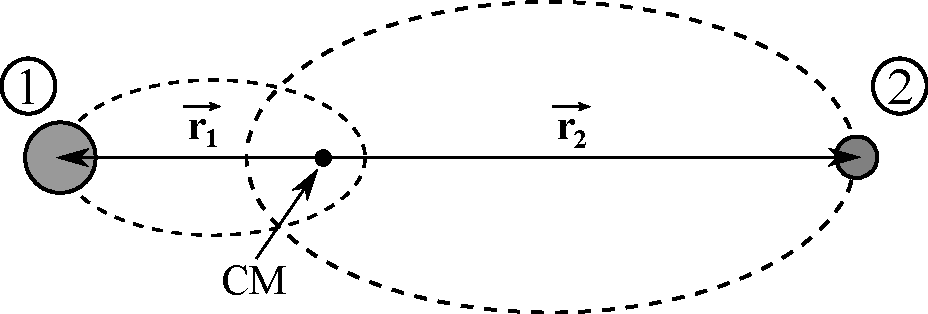
\includegraphics[width=0.95\textwidth]{Planetbevaegelse/Bevarelse_af_impulsmoment_spg1}
		\caption{Spørgsmål 1.}
		\label{fig:Bevarelse_af_impulsmoment_spg1}
	\end{subfigure}
	\hfill
	\vspace{5mm}
	\begin{subfigure}{0.49\textwidth}
		\centering
		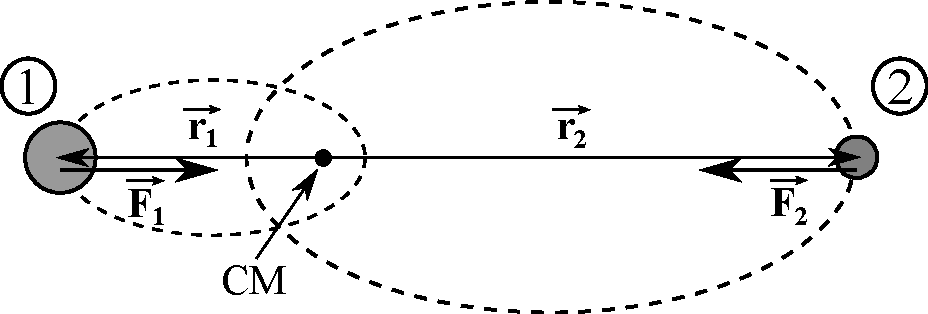
\includegraphics[width=0.95\textwidth]{Planetbevaegelse/Bevarelse_af_impulsmoment_spg2}
		\caption{Spørgsmål 2.}
		\label{fig:Bevarelse_af_impulsmoment_spg2}
	\end{subfigure}
	\begin{subfigure}{0.70\textwidth}
		\centering
		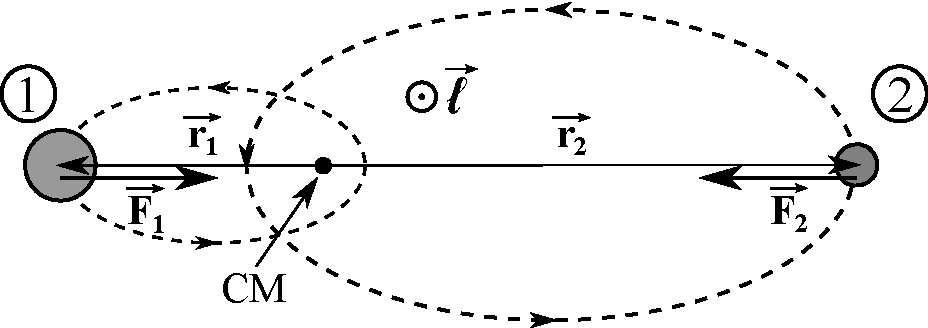
\includegraphics[width=0.95\textwidth]{Planetbevaegelse/Bevarelse_af_impulsmoment_spg5}
		\caption{Spørgsmål 5.}
		\label{fig:Bevarelse_af_impulsmoment_spg5}
	\end{subfigure}
	\caption{Grafiske besvarelser til opgave \ref{opg:Bevarelse_af_impulsmoment}. Kræfterne er på disse tegning tegnet lidt under massemidtpunktet af hvert legeme for at gøre figuren mere overskuelig.}
	\label{fig:Bevarelse_af_impulsmoment}
\end{figure}
%
\begin{opgave}{Bevarelse af impulsmoment}{1}
\opg Se figur \ref{fig:Bevarelse_af_impulsmoment_spg1}.\\
Banernes excentricitet skal være ens, mens banernes halve storakse blot er skaleret efter forholdet mellem de to legemers afstande til massemidtpunktet.
%
\opg Se figur \ref{fig:Bevarelse_af_impulsmoment_spg2}.\\
Ifølge Newtons 3. lov skal de to kræfter være lige store og modsatrettede.
%
\opg Kraftmomentet er givet ved
\begin{align*}
	\v{\tau} &= \v{r} \times \v{F} \: ,
\end{align*}
men siden det for begge legemer gør sig gældende, at $\v{r}_i \parallel \v{F}_i \: , \: \forall \, i = 1,2$, da vil krydsproduktet mellem disse to vektorer give $0$, hvorfor
\begin{align*}
	\v{\tau}_i = \v{0} \: , \enspace \forall \, i = 1,2 \: .
\end{align*}
%
\opg Af kompendiets ligning \eqref{k-eq:sum_tau_lig_aflede_impulsmoment} vides det at
\begin{align*}
	\v{\tau}_i &= \dif{t}{\v{\ell}_i} \: ,
\end{align*}
og siden det blev fundet, at $\v{\tau}_i = \v{0}$, da betyder det, at den tidsafledede af impulsmomentet er $\v{0}$, hvilket gør sig gældende, hvis impulsmomenter er konstant.\\
Idet at hvert af impulsmomenterne er konstant, da vil det også betyde, at det totale impulsmoment er konstant.
%
\opg Se figur \ref{fig:Bevarelse_af_impulsmoment_spg5}.\\
Impulsmomentet er givet ved
\begin{align*}
	\v{\ell} &= \v{r} \times \v{p} \: ,
\end{align*}
hvortil højrehåndsreglen benyttes til at finde retningen af hvert af impulsmomenterne, da retningen af  afstandsvektoren $\v{r}$ og hastigheden $\v{v}$, og dermed impulsen $\v{p}$, kendes. Retningen af de to impulsmomenter vil være den samme, hvorfor det totale impulsmoment også vil gå i denne retning.
\end{opgave}
%
%
\begin{opgave}{Keplers 3. lov}{2}
\opg Vi ved at
\begin{align*}
	P &= \frac{A}{\d A / \d t}
	= \frac{\pi a b}{\left(\dfrac{\ell}{2\mu}\right)} \\
	\Rightarrow	P^2 &= \frac{4 \pi^2 a^2 b^2 \mu^2}{\ell^2} \: .
\end{align*}
Fra kompendiets ligning \eqref{k-eq:Planetbevaegelse_a_b_og_d} vides det at
\begin{align*}
	a &= \frac{c}{1-\epsilon^2} \, \\
	b &= \frac{c}{\sqrt{1-\epsilon^2}} \: ,
\end{align*}
og udtrykkes $b^2$ ved $a^2$ bliver det
\begin{align*}
	b^2 &= a^2 \frac{(1-\epsilon^2)^2}{1-\epsilon^2}
	= a^2 (1-\epsilon^2) \: ,
\end{align*}
hvilket kan indsættes i udtrykket for $P^2$:
\begin{align*}
	P^2 &= \frac{4 \pi^2 a^2 a^2 (1-\epsilon^2) \mu^2}{\ell^2}
	= \frac{4 \pi^2 a^4 (1-\epsilon^2) \mu^2}{\ell^2} \: .
\end{align*}
Hernæst vides det fra kompendiet, at
\begin{align*}
	c &= \frac{\ell^2}{Gm_1m_2\mu} \\
	\Rightarrow \ell^2 &= Gm_1m_2\mu c \: ,
\end{align*}
hvorfor $P^2$ bliver
\begin{align*}
	P^2 &= \frac{4 \pi^2 a^4 (1-\epsilon^2) \mu^2}{Gm_1m_2\mu c}
	= \frac{4 \pi^2 a^4 (1-\epsilon^2) \mu}{Gm_1m_2 c} \: .
\end{align*}
Hernæst indsættes et udtryk for $c$ fået fra ligningen for $a$,
\begin{align*}
	c &= a(1-\epsilon^2) \: ,
\end{align*}
i udtrykket for $P^2$
\begin{align*}
	P^2 &= \frac{4 \pi^2 a^4 (1-\epsilon^2) \mu}{Gm_1m_2 a(1-\epsilon^2)}
	= \frac{4 \pi^2 a^3 \mu}{Gm_1m_2} \: .
\end{align*}
Sidst indsættes udtrykket for den reducerede masse,
\begin{align*}
	\mu &= \frac{m_1m_2}{m_1+m_2} \: ,
\end{align*}
i $P^2$:
\begin{align*}
	P^2 &= \frac{4 \pi^2 a^4 (1-\epsilon^2) \dfrac{m_1m_2}{m_1+m_2}}{Gm_1m_2 a(1-\epsilon^2)}
	= \frac{4 \pi^2}{G(m_1+m_2)}a^3 \: .
\end{align*}
\end{opgave}
%
%
\begin{opgave}{Energibevarelse og excentricitet}{3}
\opg Hastigheden skifter fortegn, når kometen passerer $r_{\mathrm{min}}$. Derved må $v(r_{\mathrm{min}}) = 0$. Af dette bliver energien i $r_{\mathrm{min}}$:
\begin{align*}
	E(r_{\mathrm{min}}) &= V_{eff}(r_{\mathrm{min}})
	= \frac{\ell^2}{2\mu r_{\mathrm{min}}^2} - \frac{\gamma}{r_{\mathrm{min}}}
	= \frac{1}{2 r_{\mathrm{min}}} \left(\frac{\ell^2}{\mu r_{\mathrm{min}}} - 2\gamma\right) \: .
\end{align*}
%
\opg Fra kompendiets ligning \eqref{k-eq:r(phi)} har vi, at
\begin{align*}
	r &= \frac{c}{1+\epsilon\cos(\phi)} \: ,
\end{align*}
hvilket for $r_{\mathrm{min}}$ bliver
\begin{align*}
	r_{\mathrm{min}} &= \frac{c}{1+\epsilon\cos(0)}
	= \frac{c}{1+\epsilon} \: .
\end{align*}
Ved at indsætte den givne værdi for $c$ fås
\begin{align*}
	r_{\mathrm{min}} &= \frac{\ell^2}{\gamma\mu(1+\epsilon)} \: .
\end{align*}
%
\opg Her indsættes resultatet fra spørgsmål 2 i resultatet fra spørgsmål 1:
\begin{align*}
	E = \frac{\gamma\mu(1+\epsilon)}{2 \ell^2} \left(\gamma(1+\epsilon) - 2\gamma\right)
	= \frac{\gamma^2\mu}{2\ell^2} (\epsilon+1)(\epsilon-1)
	= (\epsilon^2-1)\frac{\gamma^2\mu}{2\ell^2} \: .
\end{align*}
Da der er energibevarelse må denne energi være den samme, som den til en vilkårligt andet tidspunkt eller sted i banen.
%
\opg Hvis energien skal være negativ kræves, at $\epsilon^2 < 1$, altså $0\leq \epsilon < 1$. Dette er excentriciteten for en ellipsebane (eller cirkelbane hvis $\epsilon = 0$), hvilket stemmer fint overens med at kometen er i en bunden bane, når den potentielle energi er større end den kinetiske.\\
Hvis energien er $0$ kræves, at $\epsilon^2 = 1$, altså $\epsilon = 1$. Dette er svarende en parabelbane, hvor kometen netop undslipper, men dette sker så langsomt som muligt, da den kinetiske energi netop opvejer den potentielle energi.\\
Hvis energien er positiv, da må $\epsilon^2 > 1$, altså $\epsilon > 1$, hvorfor der må være tale om en hyperbelbane.
\end{opgave}
%
%
%
\section*{Baneskift}
%
%
\begin{figure}
	\centering
	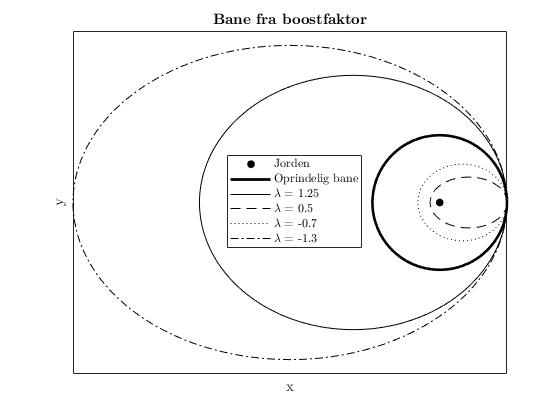
\includegraphics[width=0.85\textwidth]{Planetbevaegelse/Boostfaktor_tegninger.png}
	\caption{Baner fundet fra forskellige boostfaktorer.}
	\label{fig:Boostfaktor_tegninger}
\end{figure}
%
\begin{opgave}{Boostfaktor}{1}
Se figur \ref{fig:Boostfaktor_tegninger}. Her er forskellige værdier af de positive og negative boostfaktorer valgt, da fortegnet for boostfaktoren blot vender bevægelsesretningen.
\end{opgave}
%
%
\begin{opgave}{Boostkraft}{2}
\opg \begin{align*}
	\v{F} &= m\v{a}
	\xleq{\v{a} = \dif{t}{\v{v}}}
	m \dif{t}{\v{v}}
	= \dif{t}{m\v{v}}
	\xleq{\v{p} = m\v{a}}
	\dif{t}{\v{p}}
	= \lim\limits_{t \rightarrow 0} \frac{\Delta \v{p}}{\Delta t} \: .
\end{align*}
\opg Først finds impulsmomentet i $P$ før og efter boostet, hhv. $\ell_1$ og $\ell_2$:
\begin{align*}
	\ell_1 &= mv_1r_1 \: , \\
	\ell_2 &= mv_2r_2
	\xleq{\lambda = \frac{v_2}{v_1}}
	m \lambda v_1 r_2 \: ,
\end{align*}
hvor $m$ er satellittens masse, som antages ikke at ændre sig under boostet, $v$ er hastigheden og $r$ er afstanden mellem Jorden og satellitten.
Forskellen i impulsmoment findes:
\begin{align*}
	\Delta \ell &= \ell_2 - \ell_1
	= m \lambda v_1 r_2 - mv_1r_1
	\xleq{r_1(P) = r_2(P)}
	mv_1r_1(\lambda - 1) \: ,
\end{align*}
Da impulsmomentet findes som
\begin{align*}
	\ell &= rp \: ,
\end{align*}
så bliver ovenstående
\begin{align*}
	\Delta \ell &= r_1 \Delta p \: ,
\end{align*}
hvor
\begin{align*}
	\Delta p = mv_1(\lambda-1) \: .
\end{align*}
Boostkraften bliver dermed
\begin{align*}
	F_{av} &= \frac{\Delta p}{\Delta t}
	= \frac{mv_1}{\Delta t} (\lambda-1) \: .
\end{align*}
\end{opgave}
%
%
\begin{opgave}{Hohmannbane}{2}
\opg Hohmannbanen har apsis i de to baner med radius hhv. $R_1$ og $R_3 = 2R_1$. Da $R_3 > R_1$, må Hohmannbanen havde apoapsis i $P'$ og periapsis i $P$.
%
\opg Da bane 1 er cirkulær, så vil excentriciteten af denne bane være $\epsilon_1 = 0$. Ved brug af kompendiets ligning \eqref{k-eq:Generel_formel_r(phi)} kan det ses, at $R_1 = c_1$:
\begin{align*}
	R_1 &= \frac{c_1}{1+\epsilon_1\cos(\phi-\delta)}
	\xleq{\epsilon_1 = 0}
	\frac{c_1}{1} = c_1 \: .
\end{align*}
Excentriciteten af Hohmannbanen kan nu findes ved kompendiets ligning \eqref{k-eq:Baneskift_epsilon2}:
\begin{align*}
	\epsilon_2 &= \lambda^2\epsilon_1+(\lambda^2-1)
	\xleq{\epsilon_1 = 0}
	\lambda^2-1 \: .
\end{align*}
Idet satelitten er i apoapsis i Hohmannbanen ($P'$) skal $r_2(P') = R_3$. Der gøres her igen brug af kompendiets ligning \eqref{k-eq:Generel_formel_r(phi)}:
\begin{align*}
	R_3 &= r_2(P') = \frac{c_2}{1+\epsilon_2\cos(\pi)} = \frac{c_2}{1-\epsilon_2}
	\xleq{\epsilon_2 = \lambda^2-1}
	\frac{c_2}{1-(\lambda^2-1)} = \frac{c_2}{2-\lambda^2} \: .
\end{align*}
$c_2$ kan ved kompendiets ligning \eqref{k-eq:Baneskift_c2}:
\begin{align*}
	c_2 &= \lambda^2 c_1
	\xleq{c_1 = R_1}
	\lambda^2 R_1 \: .
\end{align*}
Indsættes dette i udtrykket for $R_3$ fra tidligere fås:
\begin{align*}
	R_3 &= \frac{\lambda^2 R_1}{2-\lambda^2} \\
	\Rightarrow \frac{R_1}{R_3} &= \frac{2-\lambda^2}{\lambda^2} = \frac{2}{\lambda^2} - 1 \\
	\Rightarrow \frac{2}{\lambda^2} &= \frac{R_1}{R_3} + 1 = \frac{R_1+R_3}{R_3} \\
	\Rightarrow \lambda^2 &= \frac{2R_3}{R_1+R_3} \\
	\Rightarrow \lambda &= \sqrt{\frac{2R_3}{R_1+R_3}}
	\xleq{R_3 = 2R_1}
	\sqrt{\frac{2 \cdot 2R_1}{R_1+2R_1}} = \sqrt{\frac{4R_1}{3R_1}} = \sqrt{\frac{4}{3}} \: .
\end{align*}
Altså vil boostfaktoren i punktet $P$ være $\lambda = \sqrt{4/3}$.
%
\opg Da bane 1 er cirkulær, så vil excentriciteten af denne bane være $\epsilon_3 = 0$. Ved brug af kompendiets ligning \eqref{k-eq:Generel_formel_r(phi)} kan det ses, at $R_3 = c_3$:
\begin{align*}
	R_3 &= \frac{c_3}{1+\epsilon_3\cos(\phi-\delta)}
	\xleq{\epsilon_3 = 0}
	\frac{c_3}{1} = c_3 \: .
\end{align*}
$c_3$ kan nu beskrives ved kompendiets ligning \eqref{k-eq:Baneskift_c2}:
\begin{align*}
	c_3 &= \lambda'^2 c_2
	\xleq{c_2 = \lambda^2 c_1}
	\lambda'^2 \lambda^2 c_1
	\xleq{c_1 = R_1}
	\lambda'^2 \lambda^2 R_1 \: .
\end{align*}
Heri isoleres nu for at finde $\lambda'$:
\begin{align*}
	\lambda'^2 &= \frac{c_3}{\lambda^2 R_1}
	\xleq{c_3 = R_3}
	\frac{R_3}{\lambda^2 R_1}
	\xleq{\lambda = \sqrt{\frac{2R_3}{R_1+R_3}}}
	\frac{R_3}{\dfrac{2R_3}{R_1+R_3} R_1}
	= \frac{R_3}{\left(\dfrac{2R_1R_3}{R_1+R_3}\right)}
	= R_3 \frac{R_1+R_3}{2R_1R_3}
	= \frac{R_1+R_3}{2R_1} \\
	\lambda' &= \sqrt{\frac{R_1+R_3}{2R_1}}
	\xleq{R_3 = 2R_1}
	\sqrt{\frac{R_1+2R_1}{2R_1}}
	= \sqrt{\frac{3R_1}{2R_1}}
	= \sqrt{\frac{3}{2}} \: .
\end{align*}
Altså vil boostfaktoren i punktet $P'$ være $\lambda' = \sqrt{3/2}$.
%
\opg Da der er impulsmomentbevarelse, da vil følgende gøre sig gældende for Hohmannbanen:
\begin{align*}
	m v_2(P)r_2(P) &= m v_2(P')r_2(P') \: ,
\end{align*}
hvor $m$ er satellittens masse, som antages konstant under hele baneskiftet, hvorfor denne går ud.\\
Herudover vides det, at $r_2(P) = R_1$ og $r_2(P') = R_3$, hvorfor ligningen bliver
\begin{align*}
	v_2(P)R_1 &= v_2(P')R_3 \: .
\end{align*}
Af formlen for boostfaktoren, kompendiets ligning \eqref{k-eq:Baneskift_boostfaktor}, fås
\begin{align*}
	\begin{aligned}
		\lambda &= \frac{v_2(P)}{v_1(P)} \\
		&\Downarrow \\
		v_2(P) &= \lambda v_1
	\end{aligned}
	\qquad \qquad
	\begin{aligned}
		\lambda' &= \frac{v_3(P')}{v_2(P')} \\
		&\Downarrow \\
		v_2(P') &= \frac{v_3}{\lambda'}
	\end{aligned}
\end{align*}
hvilket indsættes i ligningen ovenfor:
\begin{align*}
	\lambda v_1 R_1 &= \frac{v_3}{\lambda'} R_3 \: ,
\end{align*}
og $v_3$ isoleres
\begin{align*}
	v_3 &= \frac{\lambda' \lambda v_1 R_1}{R_3}
	= \sqrt{\frac{3}{2}} \sqrt{\frac{4}{3}}\frac{v_1 R_1}{R_3}
	= \sqrt{\frac{12}{6}} \frac{v_1 R_1}{R_3}
	\xleq{R_3 = 2R_1}
	\sqrt{2} \frac{v_1 R_1}{2R_1}
	\xleq{\frac{\sqrt{2}}{2} = \frac{1}{\sqrt{2}}}
	\frac{1}{\sqrt{2}} v_1 \: .
\end{align*}
Altså er hastigheden af satellitten i den nye bane udtrykt ved hastigheden i begyndelsesbanen $v_3 = v_1/\sqrt{2}$.
\end{opgave}
%
%
\begin{opgave}{Hohmannbane II}{2}
Fra opgave \ref{opg:Hohmannbane} blev det fundet, at boostfaktoren for et skift mellem fra en startbane til en Hohmannbane er givet ved
\begin{align} \label{eq:Boostfaktor_generel}
	\lambda &= \sqrt{\frac{2R_{\text{efter}}}{R_{før}+R_{\text{efter}}}} \: ,
\end{align}
og boostfaktoren for et skift mellem Hohmannbanen og slutbanen er givet ved
\begin{align} \label{eq:Boostfaktor_maerke_generel}
	\lambda' &= \sqrt{\frac{R_{\text{før}}+R_{\text{efter}}}{2R_{\text{før}}}} \: ,
\end{align}
hvor $R_{\text{før}}$ er radius af den første bane, altså banen inden skiftet til Hohmannbanen, og $R_{\text{efter}}$ er radius af den sidste bane, altså banen der kommer af skiftet fra Hohmannbanen.
%
\opg Der er tale om et skift fra en cirkulær bane (A) til en Hohmannbane (1), hvorfor ligning \eqref{eq:Boostfaktor_generel} bruges. Her er $R_{\text{før}} = R_A$ og $R_{\text{efter}} = R_C = (9/2)R_A$:
\begin{align*}
	\lambda_1 &= \sqrt{\frac{2\cdot \dfrac{9}{2}R_A}{R_A+\dfrac{9}{2}R_A}}
	= \sqrt{\frac{9R_A}{\dfrac{11}{2}R_A}}
	= \sqrt{\frac{18R_A}{11R_A}}
	= \sqrt{\frac{18}{11}} \: .
\end{align*}
%
\opg Der er tale om et skift fra en Hohmannbane (1) til en cirkulær bane (C), hvorfor ligning \eqref{eq:Boostfaktor_maerke_generel} bruges. Her er $R_{\text{før}} = R_A$ og $R_{\text{efter}} = R_C = (9/2)R_A$:
\begin{align*}
	\lambda_1' &= \sqrt{\frac{R_A+\dfrac{9}{2}R_A}{2R_A}}
	= \sqrt{\frac{\dfrac{11}{2}R_A}{2R_A}}
	= \sqrt{\frac{11}{4}\frac{R_A}{R_A}}
	= \sqrt{\frac{11}{4}} \: .
\end{align*}
%
\opg Der er tale om et skift fra en cirkulær bane (C) til en Hohmannbane (2), hvorfor ligning \eqref{eq:Boostfaktor_generel} bruges. Her er $R_{\text{før}} = R_C = (3/2)R_B$ og $R_{\text{efter}} = R_B$:
\begin{align*}
	\lambda_2 &= \sqrt{\frac{2R_B}{\dfrac{3}{2}R_B+R_B}}
	= \sqrt{\frac{2R_B}{\dfrac{5}{2}R_B}}
	= \sqrt{\frac{4R_B}{5R_B}}
	= \sqrt{\frac{4}{5}} \: .
\end{align*}
\opg Der er tale om et skift fra en Hohmannbane (2) til en cirkulær bane (B), hvorfor ligning \eqref{eq:Boostfaktor_maerke_generel} bruges. Her er $R_{\text{før}} = R_C = (3/2)R_B$ og $R_{\text{efter}} = R_B$:
\begin{align*}
	\lambda_2' &= \sqrt{\frac{\dfrac{3}{2}R_B+R_B}{2\cdot\dfrac{3}{2}R_B}}
	= \sqrt{\frac{\dfrac{5}{2}R_B}{3R_B}}
	= \sqrt{\frac{5}{6}\frac{R_B}{R_B}}
	= \sqrt{\frac{5}{6}} \: .
\end{align*}
%
\opg Boostfaktorerne $\lambda_1$ og $\lambda_2$ er på samme form, formen fra ligning \eqref{eq:Boostfaktor_generel}, mens boostfaktorerne $\lambda_1'$ og $\lambda_2'$ er på samme form, formen fra ligning \eqref{eq:Boostfaktor_maerke_generel}.
\end{opgave}
\chapter{Matematik}
%%
%%
\section{Polære Koordinater, Cosinus og Sinus}
%%
%%
\begin{opgave}{Idiotformlen}{1}
Brug at $\cos \theta$ og $\sin \theta$ er hhv. den hosliggende og modstående katete i en retvinklet trekant med hypotenuse 1 pr. deres definition. Tegn det i enhedscirklen. Det giver da, at $\cos^2 (\theta) + \sin^2 (\theta) = 1^2 = 1$ fra Pythagoras sætning. 
\end{opgave}
%%
%%
\begin{opgave}{Tangens}{1}
Fra definitionen af tangens har vi, at $\tan(\theta) = \sin(\theta)/\cos(\theta)$. Men i matematikafsnittet er det også introduceret, at $\cos(\theta)$ er givet som længden af den hosliggende katete divideret med længden af hypotenusen, og at $\sin(\theta)$ er givet som længden af den modstående katete divideret med længden af hypotenusen. 
\begin{align*}
gg
\end{align*}
\end{opgave}
\section*{Differentialregning}
\begin{opgave}{Afledte og dobbeltafledte}{1}
\opg $f(x) = x^3$: 
\begin{equation*}
\dif{x}{f}=3x^2,~~ \dif[2]{x}{f}=6x
\end{equation*}
\opg $f(x) = x^2 + 4x$:
\begin{equation*}
\dif{x}{f}=2x+4,~~ \dif[2]{x}{f}=2
\end{equation*}
\opg $f(x) = \frac{1}{x} + \frac{1}{x^2}=x^{-1}+x^{-2}$: 
\begin{equation*}
\dif{x}{f} = - x^{-2}-2x^{-3}, ~~\dif[2]{x}{f}=2x^{-3}+6x^{-4}
\end{equation*}
\opg $f(x) = \cos (x)$: 
\begin{equation*}
\dif{x}{f}= - \sin (x),~~ \dif[2]{x}{f}=-\cos (x)
\end{equation*}
\opg $f(x) = \ln (x)$: 
\begin{equation*}
\dif{x}{f}= \frac{1}{x}=x^{-1},~~\dif[2]{x}{f}=-x^{-2}
\end{equation*}
\end{opgave}

\begin{opgave}{Ubestemte integraler}{1}
\opg $f(x) = x^3$: 
\begin{equation*}
\int f(x) \d x = \frac{1}{4}x^4 +C
\end{equation*}
\opg $f(x) = x^2 + 4x$:
\begin{equation*}
\int f(x) \d x = \frac{1}{3}x^3 + 2x^2 + C
\end{equation*}
\opg $f(x) = \frac{1}{x} + \frac{1}{x^2}=x^{-1}+x^{-2}$: 
\begin{equation*}
\int f(x) \d x = \ln (x) -x^{-1} + C
\end{equation*}
\opg $f(x) = \cos (x)$: 
\begin{equation*}
\int f(x) \d x = \sin(x)+C
\end{equation*}
\opg $f(x) = \ln (x)$: 
\begin{equation*}
\int f(x) \d x = x\ln (x) -x + C
\end{equation*}
\end{opgave}

\begin{opgave}{Sammensatte funktioner}{1}
$g(x)$ og $f(g)$ findes. $\dif{x}{f}$ findes vha. kædereglen: $\dif{x}{f} = \dif{x}{g} \cdot \dif{g}{f}$.
\opg $f(x) = \sin (4x)$:
\begin{align*}
g(x) &= 4x, ~~f(g)=\sin(g) \\
\rightarrow &\dif{x}{f} = 4\cos(4x)
\end{align*}
\opg $f(x) = \sqrt{2x}$:
\begin{align*}
g(x) = 2x, ~~ f(g)=\sqrt{g} \\
\rightarrow \dif{x}{f} = 2\frac{1}{2\sqrt{2x}}=\frac{1}{\sqrt{2x}}
\end{align*}
\opg $f(x) = \sqrt{4x+5}$
\begin{align*}
g(x) = 4x+5, ~~f(g)=\sqrt{g} \\
\rightarrow \dif{x}{f} = 4\frac{1}{2\sqrt{4x+5}}=\frac{2}{\sqrt{4x+5}}
\end{align*}
\opg $f(x) = \sin(e^x)$
\begin{align*}
g(x) = e^x, ~~f(g)=\sin(g) \\
\rightarrow \dif{x}{f} = e^x \cos(e^x)
\end{align*}
\end{opgave}

\begin{opgave}{Integration ved substitution}{1}
Udregn de følgende integraler vha. integration ved substitution:
\opg $\int e^{-4x} \d x$
\begin{align*}
\int e^{-4x} \d x = -\frac{1}{4}e^{-4x} + C
\end{align*}
\opg $\int \sqrt{3x-2} \d x$
\begin{align*}
\int \sqrt{3x-2} \d x = \frac{2}{9}\cdot(3x-2)^{\frac{3}{2}} + C
\end{align*}
\opg $\int xe^{-3x^2} \d x$
\begin{align*}
\int xe^{-3x^2} \d x = -\frac{1}{6}e^{-3x^2}+C
\end{align*}
\opg $\int \frac{x-1}{\sqrt{x+1}} \d x$
\begin{align*}
\int \frac{x-1}{\sqrt{x+1}} \d x = \frac{2}{3}\sqrt{x+1}(x-5)
\end{align*}
\end{opgave}

\begin{opgave}{$\boldsymbol{f}$ som funktion af $\boldsymbol{g}$}{1}
Udtryk $\d{f}{x}$ vha. den ukendte funktion $g(x)$ og dens
differentierede $\dif{x}{g}$ for følgende funktioner:
\opg $f(x) = x^2 g(x)$. Produktreglen anvendes:
\begin{equation*}
\dif{x}{f} = \dif{x}{x^2}\cdot g(x) + x^2\dif{x}{g} = 2xg(x)+x^2 \dif{x}{g}
\end{equation*}
\opg $f(x) = \left(g(x)\right)^2$. Produktreglen anvendes:
\begin{equation*}
\dif{x}{f} = \dif{x}{g} g(x) + g(x)\dif{x}{g} = 2g(x)\dif{x}{g}
\end{equation*}
\opg $f(x) = g(x^2)$. Kædereglen anvendes:
\begin{equation*}
\d{f}{x}=2x\d{g}{x^2}
\end{equation*}
\end{opgave}

\begin{opgave}{Partiel integration}{2}
Udregn de følgende integrale vha. partiel integration og substitution:
\opg $\int 4x\cos(2-3x)\d x$
\begin{align*}
	\int 4x\cos(2-3x)\d x = \frac{4}{9}\cos(2-3x)-\frac{4}{3}x\sin(2-3x) +C
\end{align*}
\opg $\int (2+5x)e^{\frac{1}{3}x}\d x$
\begin{align*}
	\int (2+5x)e^{\frac{1}{3}x}\d x = (15x-39)e^{\frac{1}{3}x}+C
\end{align*}
\opg $\int (3x+x^2)\sin (2x) \d x$
\begin{align*}
	\int (3x+x^2)\sin (2x) \d x = -\frac{1}{2}(3x+x^2)\cos (2x) +\frac{1}{4}\Big[ (3+2x)\sin (2x) + \cos (2x) \Big] + C
\end{align*}
\end{opgave}

\begin{opgave}{Hastighed og postion}{1}
\begin{figure}[h!]
  \centering
%  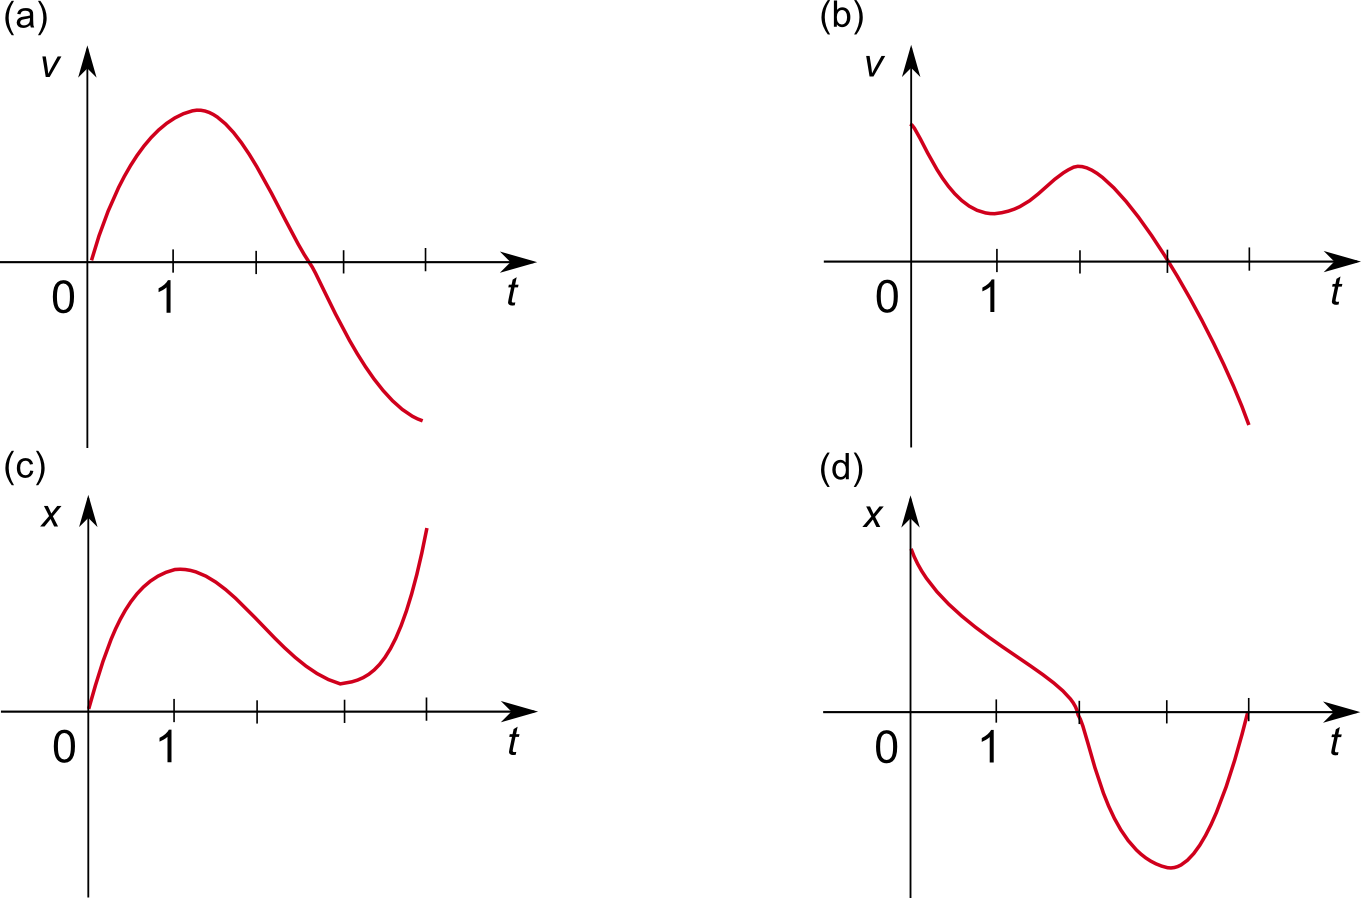
\includegraphics[width=0.6\textwidth]{matematik/vx_grafer.png}
  \caption{Hastighed og position som funktion af tiden.}
  \label{fig:vx_grafer}
\end{figure}
\opg Da grafen simpelt viser $v$ som funktion af tiden kan man bare aflæse på figuren.
for (a): 
\begin{itemize}
\item $t= 0 \rightarrow 1,5$: sætter farten op
\item $t= 1,5 \rightarrow 4$: sætter farten ned
\end{itemize}
for (b):
\begin{itemize}
\item $t= 0 \rightarrow 1$: sætter farten ned
\item $t= 1 \rightarrow 2$: sætter farten op
\item $t= 2 \rightarrow 4$: sætter farten ned
\end{itemize}
.
\opg Her ses i stedet positionen som funktion af tiden. For at svare på, hvordan hastigheden opfører sig, så skal vi derfor kigge på \emph{hældningen} af grafen.
for (c): 
\begin{itemize}
\item $t= 0 \rightarrow 1$: positiv hældning $\rightarrow$ hastigheden øges
\item $t= 1 \rightarrow 3$: negativ hældning $\rightarrow$ hastigheden sænkes
\item $t= 3 \rightarrow 4$: positiv hældning $\rightarrow$ hastigheden øges
\end{itemize}
for (d):
\begin{itemize}
\item $t= 0 \rightarrow 2$: negativ hældning $\rightarrow$ hastigheden sænkes
\item $t= 2 \rightarrow 3$: negativ hældning $\rightarrow$ hastigheden sænkes - og hældningen er større, så der bremses hårdere.
\item $t= 3 \rightarrow 4$: positiv hældning $\rightarrow$ hastigheden øges
\end{itemize}
.
\end{opgave}
\begin{opgave}{Harmonisk bevægelse}{2}
\begin{equation*}
x = A \cos (\omega t + \phi),
\end{equation*}
hvor $A$, $\omega$ og $\phi$ er konstanter. 
\opg For at finde hastigheden ($\dt{x}$), så ses det at udtrykket er en sammensat funktion ($g=\omega t+\phi$, $f=A\cos g$). Bruges kædereglen får man:
\begin{equation*}
\dt{x} = - A\omega \sin(\omega t + \phi)
\end{equation*}
\opg Hvis det antages at alle konstanter er $>0$, så er $\dt{x}=0$, når $\sin(\omega t + \phi) = 0$. Det er opfyldt for $\omega t + \phi = 0, \pi, 2\pi, ...$. Fysisk set er $v=0$ i yderpunkterne af svingningen, som forekommer periodisk.
\end{opgave}
\begin{opgave}{Cepheide-stjernen Delta Cephei}{2}
\begin{equation*}
B(t) = 4,0 + 0,35\sin \left( \frac{2\pi t}{5,4} \right).
\end{equation*}
\opg Raten er $\dif{t}{B} = \dt{B}$. Funktionen er en sammensat funktion ($u=\frac{2\pi t}{5,4}, g=0,4+0,35 \sin u$).
\begin{equation*}
\dt{B} = 0,35 \cdot \frac{2\pi}{5,4} \cos \left( \frac{2\pi t}{5,4} \right)
\end{equation*}
\opg For at finde ændringen i lysstyrke udregnes forskellen:
\begin{align*}
B(t=\text{2 dage})-B(t=\text{0 dage}) \\
&= 4,0 + 0,35\sin\left(\frac{2\pi}{5,4} \cdot 2 \right) - 4,0 -0,35\sin\left(\frac{2\pi}{5,4} \cdot 0 \right) \\
&= 0,25
\end{align*}
Husk at regne i radianer og ikke i grader.
\end{opgave}

\begin{opgave}{Udvidelse af ballon}{2}
\opg $\dif{r}{V}$ er ændring af volumen afhængig af radius, mens $\dif{t}{V}$ er ændring af volumen afhængig af tiden.
\opg Volumenet af en sfærisk ballon er $V(t)=\frac{4}{3} \pi r(t)^3$. Det er en sammensat funktion med $u=r(t)$ og $g=\frac{4}{3} \pi u^3$. Det giver:
\begin{equation*}
\dt{V} = \frac{4}{3} 2\pi \cdot 3 r^2(t) \dt{r}
\end{equation*}
\end{opgave}

\begin{opgave}{Approksimation af funktion}{3}
  \[
  f(x) = f(a) + (x-a) \left.\d{f}{x}\right|_{x=a}
  + \frac{1}{2} (x-a)^2 \left.\dif[2]{x}{f}\right|_{x=a}
  + \frac{1}{3!} (x-a)^3 \left.\dif[3]{x}f\right|_{x=a}
  + \ldots
  \]
  \opg Første led er en konstant, mens andet led afhænger linært af $x$, og tredje led kvadratisk af $x$ osv. Forfaktoren bliver mindre og mindre for hvert led, så ledene bliver mindre og mindre.
  \opg For $x \approx 0$, er $\sin (x)$ med de første to led:
  \begin{align*}
  \sin x &= \sin(0) + (x-0) \left. \dif{x}{\sin (x)}\right|_{x=0} \\
  &= 0 + x\cos(0) \\
  &= x
  \end{align*}
  Idet $\sin(0)=0$ og $\cos(0)=1$.
  For $x \approx 0$, er $\cos x$ med de første to led:
  \begin{align*}
  \cos (x) &= \cos(0) + (x-0) \left.\dif{x}{\sin (x)}\right|_{x=0} \\
  &= 1 -x\sin(0) \\
  &= 1
  \end{align*}
  Hvis man medtager det 3. led, så bliver $\sin(x)$:
  \begin{align*}
  \sin(x) &= x + \frac{1}{2} (x-0)^2 \left. \dif[2]{x}{\sin(x)}\right|_{x=0} \\
  &= x - \frac{x^2}{2} \sin(0) \\
  &= x  
  \end{align*}
  Hvis man medtager det 3. led, så bliver $\cos(x)$:
  \begin{align*}
  \cos(x) &= 1 + \frac{1}{2} (x-0)^2 \left.\dif[2]{x}{\cos(x)}\right|_{x=0} \\
  &= 1 - \frac{x^2}{2} \cos(0) \\
  &= 1 - \frac{x^2}{2}  
  \end{align*}
  \opg For $x \approx 1$, er $\ln (x)$ for de tre første to led:
  \begin{align*}
  \ln x &= \ln(1) + (x-1) \left. \dif{x}{\ln (x)} \right|_{x=1} + \frac{1}{2} \left(x-1\right)^2 \left. \dif[2]{x}{\ln (x)}\right|_{x=1} \\
  &= 0 + (x-1)\frac{1}{1} - \frac{1}{2} \left( x^2 +1 - 2x \right) \left. \dif{x}{} \frac{1}{x} \right|_{x=1} \\
  &= x -1 + \frac{1}{2} \left( x^2 + 1 - 2x \right) \left. \left( -1 x^{-2} \right)\right|_{x=1} \\
  &= x - 1 - \frac{x^2}{2} - \frac{1}{2} + x\\
  &= - \frac{x^2}{2} + 2x - \frac{3}{2}
  \end{align*}
  Idet den differentierede at $\ln (x) = \frac{1}{x}$ og $\ln (1)=0$.
  \opg For $x \approx 0$, er $e^x \approx 1 + x + \frac{1}{2}
  x^2$ for de første tre led:
  \begin{align*}
  e^x &= e^0 + (x-0) \left. \dif{x}{e^x}\right|_{x=0} + \frac{1}{2}(x-0)^2 \left. \dif[2]{x}{e^x}\right|_{x=0} \\
  &=1 + x + \frac{1}{2} x^2,
  \end{align*}
  Idet den differentierede af $e^x$ er $e^x$ og $e^0 = 1$.
  \opg For $x \approx 0$, vises det, at approksimationen for et polynomie
  $a_0 + a_1 x + a_2 x^2 + \ldots$ er givet ved leddene i polynomiet
  selv. Vi regner ét led af gangen:
  \begin{align*}
  \text{Første led } &= a_0 + a_1\cdot 0 + a_2 \cdot 0^2 \\
  &= a_0 \\
  \text{Andet led } &= (x-0) \left. \dif{x}{} \left(a_0 + a_1x + a_2x^2 \right)\right|_{x=0} \\
  &= x \cdot \left. \left(a_1 + 2a_2x) \right)\right|_{x=0} \\
  &= a_1 x \\
  \text{Tredje led} &= \frac{1}{2} \left( x-0 \right)^2 \left. \dif[2]{x}{} \left(a_0 + a_1x + a_2x^2 \right)\right|_{x=0} \\
  &= \frac{1}{2} x^2 \left. \dif{x}{} \left(a_1 + 2a_2x \right)\right|_{x=0} \\
  &= \frac{1}{2} x^2 \left. \left( 2a_2 \right)\right|_{x=0} \\
  &= a_2 x^2 \\
  \rightarrow & a_0 + a_1x+a_2x^2
  \end{align*}
  Og det er hermed vist at approksimationen af et polynomie er givet ved leddene i polynomiet.
  \opg For små værdier af $x$ ($x \approx 0$), vises det, at $(1 + x)^a \approx 1 + ax$.:
  \begin{align*}
  (1+x)^a &= (1+0)^a + (x-0) \left. \dif{x}{(1+x)^a}\right|_{x=0} \\
  &= 1 + \left. \left( a(1+x)^{a-1} \right)\right|_{x=0} \\
  &= 1 + ax,
  \end{align*}
  hvor $(1+x)^a$ er blevet differentieret som en sammensat funktion med $u=1+x$ og $g=u^a$.
\end{opgave}

\begin{figure}
	\centering
%	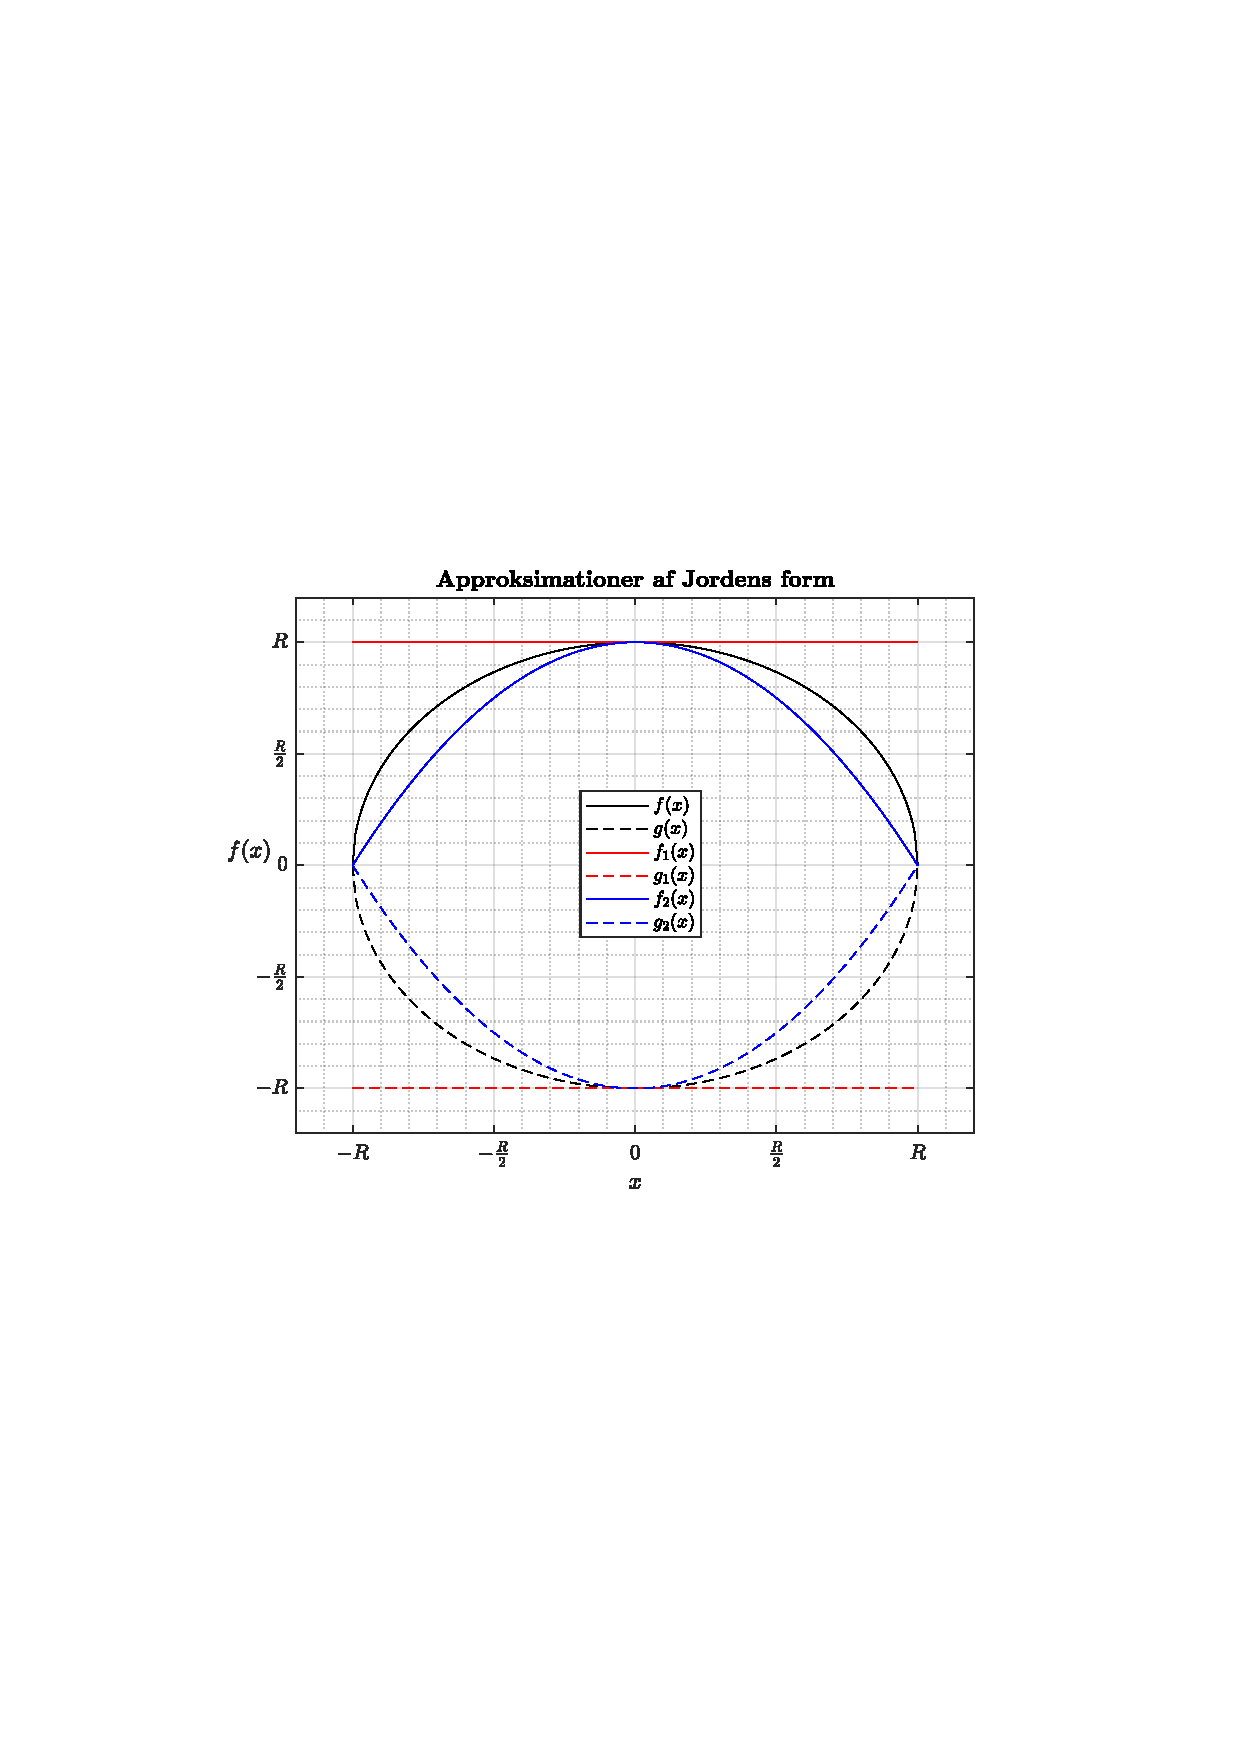
\includegraphics[width=\columnwidth]{/matematik/fig/JordensForm.pdf}
	\caption{Plot af $f(x),g(x)$, samt approksimationer af disse.} \label{fig:JordensForm}
\end{figure}
\begin{opgave}{Jordens form}{2}
I første omgang differentieres funktionen to gange vha. kædereglen
\begin{align*}
	\dif{x}{f(x)} &= \frac{1}{2}\left[R^2 - x^2\right]^{-1/2}(-2x) \\
	&= \frac{-x}{\sqrt{R^2 - x^2}} \\
	\dif[2]{x}{f(x)} &= \dif{x}{}\left(\frac{-x}{\sqrt{R^2 - x^2}}\right) \\
	&= -\frac{1}{2}\left[R^2 - x^2\right]^{-3/2}(-x)(-2x) - \left[R^2 - x^2\right]^{-1/2} \\
	&= \frac{-x^2}{(R^2 - x^2)^{3/2}} - \frac{1}{\sqrt{R^2 - x^2}}
\end{align*}
Evalueres disse differentialer i $x = 0$ fås
\begin{align*}
	\left.\dif{x}{f(x)}\right|_{x=0} &= \left[\frac{-x}{\sqrt{R^2 - x^2}}\right]_{x=0} \\
	&= \frac{-0}{\sqrt{R^2 - 0^2}} \\
	&= 0 \\
	\left.\dif[2]{x}{f(x)}\right|_{x=0} &= \left[\frac{-x^2}{(R^2 - x^2)^{3/2}} - \frac{1}{\sqrt{R^2 - x^2}}\right]_{x=0} \\
	&= \frac{-0^2}{(R^2 - 0^2)^{3/2}} - \frac{1}{\sqrt{R^2 - 0^2}} \\
	&= 0 - \frac{1}{R} \\
	&= -\frac{1}{R}
\end{align*}
\opg Indsættes det i ligning \ref{k-Taylor_pol} fra kompendiet fås
\begin{align*}
	f_2(x) &\simeq f(0) + x\left.\dif{x}{f(x)}\right|_{x=0} + \frac{1}{2}x^2\left.\dif[2]{x}{f(x)}\right|_{x=0} \\
	&= R + 0 - \frac{1}{R}x^2
\end{align*}
hvilket er Taylorrækken til 2. orden. Til første og nulte orden er det
\begin{align*}
	f_1(x) &\simeq R + 0 = R \\
	f_0(x) &\simeq R
\end{align*}
\opg Da $f_0(x) = f_1(x)$ betragtes de herfra sammen. \\
1) \enspace $f_1$ er en vandret linje for alle værdier af $x$ \\
2) \enspace $f_2(x)$ er en parabel, hvor "benene" vender nedad, grundet fortegnet på højesteordensledet.
\opg Se figur \ref{fig:JordensForm}.
\opg Der er tale om \\
1) \enspace Et plan. \\
2) \enspace En elliptisk paraboloid, dvs. den figur, der fremkommer ved at dreje en parabel\SI{180}{\degree} rundt om $y$-aksen. Af denne figur er taget de positive værdier og spejlet i $x$-aksen. Denne forklaring giver ikke super meget mening, hvorfor det er bedre bare at tænke det som et øje.
\opg På bagrund af dette er det acceptable approksimationer at se jorden som enten flad eller et gigantsisk øje. Som figuren dog viser er det begrænset, hvor stort et område disse approksimationer er valide.
\end{opgave}

\newpage

\section*{Differentialligninger}

\begin{opgave}{Specialtilfælde af 1. og 2. Ordens Differentialligninger}{1}
\opg $f(t) = -7e^{3t}$ og $\dif{t}{f} = 3f(t)$.

$$\dif{t}{f} = -7 \dif{t}{} e^{3t} = -7 \cdot 3 e^{3t} = 3 \left( -7 e^{3t} \right) = 3 f(t)$$
\vspace{2mm}
\opg $g(t) = \frac{2}{3}e^t + e^{-2t}$ og $\dif{t}{g} + 2g(t) = 2e^t$.

$$\dif{t}{g} = \frac{2}{3} \dif{t}{}e^t + \dif{t}{} e^{-2t} = \frac{2}{3}e^t -2e^{-2t} \quad \Rightarrow \quad \dif{t}{g} + 2g(t) = \frac{2}{3}e^t -2e^{-2t} + \frac{4}{3}e^t + 2e^{-2t} = \frac{6}{3} e^t = 2e^t$$
\vspace{2mm}
\opg $h(t) = 5 \sin(3t) - 10\cos(3t)$ og $\dif[2]{t}{h} = -9h(t)$.

$$\dif{t}{h} = 3 \cdot 5 \cos(3t) + 3 \cdot 10 \sin(3t) \quad \Rightarrow \quad \dif[2]{t}{h} = (-9) \cdot 5 \cos(3t) + 9 \cdot 10 \sin(3t) = -9 h(t)$$
\vspace{2mm}
\opg $k(t) = 13 \cos \left( 8t + 45 \right)$ og $\dif[2]{t}{k} = -64 k(t)$.

$$\dif{t}{k} = (-8) \cdot 13 \cos \left( 8t + 45 \right) \quad \Rightarrow \quad \dif[2]{t}{k} = (-64) \cdot 13 \cos \left( 8t + 45 \right) = -64 k(t)$$
\vspace{2mm}
\end{opgave}

\begin{opgave}{Generelle 1. Ordens Differentialligninger}{2}
\opg $h(x) = 1/ \left( x+A \right)$ og $\dif{x}{h} = -h(x)^2$.

$$\dif{x}{f} = \dif{x}{}\left( x+A \right)^{-1} = - \left( x+A \right)^{-2} \dif{x}{}\left( x+A \right) = - \frac{1}{\left( x + A \right)^2} = -h(x)^2$$
\vspace{2mm}
\opg $k(x) = \left( c-x^2 \right)^{-1/2}$ og $\d{k}{x} = x k(x)^3$.

$$\dif{x}{k} = - \frac{1}{2} \left( c-x^2 \right)^{-3/2}  \dif{x}{}\left( c-x^2 \right) = x \left( c-x^2 \right)^{-3/2} = x k(x)^3$$
\vspace{2mm}
\opg $g(x) = \left( \ln (x) + C \right)/x$ og $x^2 \dif{x}{g} + x g(x) = 1$.

\begin{align*}
	\dif{x}{g} &= \left[ \dif{x}{}\left( \ln x + C \right) \right] \frac{1}{x} + \left( \ln x + C \right)  \left[ \dif{x}{}\frac{1}{x} \right]  = \frac{1}{x^2} - \frac{\ln x + C}{x^2} \\ &\Rightarrow x^2 \dif{x}{g} + xg(x) = 1 - \left( \ln (x) + C \right) + \left( \ln (x) + C \right) = 1
\end{align*}
\vspace{2mm}
\opg $f(x) = \left( 1+ce^x \right)/\left( 1-ce^x \right)$ og $\dif{x}{f} = \frac{1}{2} \left( f(x)^2 -1 \right)$.

\begin{align*}
\dif{x}{f} &= \left[ \dif{x}{}\left( 1+c^x \right) \right] \frac{1}{1-ce^x} + \left( 1+ce^x \right) \left[ \dif{x}{}\frac{1}{1-ce^x} \right] = \frac{ce^x}{1-ce^x} +  \frac{\left( 1+ce^x \right) \left( -1 \right) \left( -ce^x \right)}{\left( 1-ce^x \right)^2}\\\\
&= ce^x \left[ \frac{1}{1-ce^x} + \frac{1+ce^x}{\left( 1-ce^x \right)^2} \right] = ce^x \frac{1-ce^x + 1+ce^x}{\left( 1-ce^x \right)^2} = \frac{2ce^x}{\left( 1-ce^x \right)^2}
\end{align*}

\begin{align*}
	f(x)^2 - 1  &=  \frac{\left( 1+ce^x \right)^2}{\left( 1-ce^x \right)^2} - \frac{(1-ce^x)^2}{\left( 1-ce^x \right)^2} = \frac{\left( 1+ce^x \right)^2 - \left( 1-ce^x \right)^2}{\left( 1-ce^x \right)^2} = \frac{4ce^x}{\left( 1-ce^x \right)^2} \\
	&\Rightarrow \dif{x}{f} = \frac{1}{2} \left( f(x)^2 -1 \right)
\end{align*}
\end{opgave}

\begin{opgave}{Hvornår er det en løsning?}{3}
\opg Find $k$ så $f(y) = \cos(ky)$ løser $4 \dif[2]{y}{f} = -25f(y)$.

$$\dif{y}{f} = -k\sin(ky) \quad \Rightarrow \quad \dif[2]{y}{f} = -k^2 \cos(ky) = -k^2 f(y)$$

\vspace{2mm}

Så sætter man ind:

$$4 \dif[2]{y}{f} = -25f(y) \quad \Rightarrow \quad -4k^2 f(y) = -25f(y) \quad \Rightarrow \quad k^2 = \frac{25}{4} \quad \Rightarrow \quad k = \pm \frac{5}{2}$$
\vspace{2mm}
\opg For de fundne $k$ fra 1), vis at $g(y) = A\sin(ky) + B\cos(ky)$ løser $4 \dif[2]{y}{g} = -25g(y)$.

$$\dif{y}{g} = kA\cos(ky) - kB\sin(ky) \quad \Rightarrow \quad \dif[2]{y}{g} = -k^2 A \sin(ky) - k^2 B \cos(ky) = -k^2g(y)$$

\vspace{2mm}

Det giver:

$$-4k^2 g(y) = -25g(y) $$

\vspace{2mm}

Som er opfyldt for $k = \pm \frac{5}{2}$.\\
\opg Find $r$ så $h(y) = e^{ry}$ løser $2 \dif[2]{y}{h} + \dif{y}{h} - h(y) = 0$.

$$\dif{y}{h} = re^{ry} = rh(y) \quad \Rightarrow \quad \dif[2]{y}{h} = r^2 e^{ry} = r^2 h(y)$$

\vspace{2mm}

Så sætter man ind:

$$2 \dif[2]{y}{h} + \dif{y}{h} - h(y) = 0 \quad \Rightarrow \quad 2r^2h(y) + rh(y) -h(y) = 0 \quad \Rightarrow \quad 2r^2+r-1=0$$
\vspace{2mm}

Løses andengradsligningen får man:

$$r_1 = \frac{1}{2} \quad \text{og} \quad r_2 = -1$$ 
\vspace{2mm}
\opg For de fundne $r_1,r_2$ i 3), vis at $k(y) = ae^{r_1y} + be^{r_2y}$ løser $2 \dif[2]{y}{k} + \dif{y}{k} - k(y) = 0$.

$$\dif{y}{k} = ar_1e^{r_1y} + br_2e^{r_2y} \quad \Rightarrow \quad \dif[2]{y}{k} = ar_1^2e^{r_1y} + br_2^2e^{r_2y}$$ 
\vspace{2mm}

Så sætter man ind:

\begin{align*}
2 \dif[2]{y}{k} + \dif{y}{k} - k(y) &= 2 \left( ar_1^2e^{r_1y} + br_2^2e^{r_2y}  \right) + \left( ar_1e^{r_1y} + br_2e^{r_2y} \right) - \left( ae^{r_1y} + be^{r_2y} \right)\\\\ 
&= \left( 2ar_1^2 + ar_1 - a \right)e^{r_1y} + \left( 2br_2^2 + br_2 - b \right)e^{r_2y} = 0 \cdot e^{r_1y} + 0 \cdot e^{r_2y} = 0 
\end{align*}
\end{opgave}


%\backmatter

%\printbibliography % BibLaTeX

%\bibliography{bach}{} % ikke BibLaTeX
%\bibliographystyle{alpha} % ikke BibLaTeX

\end{document}

